\chapter{基于监督学习的智能协议与参数联合选择方法}

\label{chapter5: ai_selector}
现代无线网络，尤其是物联网场景，业务需求呈现出显著的多样性与动态性。不同业务在接入密度、数据包长度及时延敏感度等方面差异明显，使得单一随机接入协议难以在复杂多变的网络条件下始终保持最优性能。传统基于固定协议与静态参数配置的设计，难以同时兼顾吞吐量、时延、公平性、信令开销多维性能指标，存在明显局限。
不同随机接入协议在吞吐性能、时延特性、信令开销方面表现各异。表~\ref{tab:protocol_comparison} 对 SA、SAST、CBA三种协议进行定性对比，可以看出，协议机制的增强虽可显著提升系统吞吐，但同时也可能带来更高的信令开销，进一步表明难以依靠单一协议适应所有场景。

\begin{table}[htbp]
\centering
\caption{不同随机接入协议的定性性能对比}
\label{tab:protocol_comparison}
% \renewcommand{\arraystretch}{1.2}
\begin{tabular}{c|c|c|c}
\hline
\textbf{协议} & \textbf{吞吐性能} & \textbf{时延特性} & \textbf{信令开销} \\
\hline
SA & 低 & 低 & 中 \\
\hline
SAST & 中 & 中 & 低 \\
\hline
CBA & 高 & 中-高 & 高 \\
\hline
\end{tabular}
\end{table}
因此，依据场景特征动态选择接入协议并联合优化其关键参数，是提升系统整体性能的有效途径。围绕这一需求，本章研究如何在多协议共存的统一框架下，根据业务流量状态智能决策最优协议及其参数配置。
针对此问题，本文提出一种面向动态业务场景的、基于监督学习的协议与参数联合选择方法，实现接入策略由静态向与数据驱动转变，从而在吞吐量、时延与公平性等多维性能之间取得更优平衡。

\section{问题建模与统一接入框架设计}
本节给出统一问题建模与接入框架。核心目标是在动态流量下实现协议与参数的联合自适应选择，以提升系统整体性能。
具体地，\ref{subsec:problem_formulation}小节给出联合优化问题建模，\ref{subsec:unified_input}小节构造统一输入特征，\ref{subsec:sim_mapping_utility}小节定义仿真映射与效用函数，\ref{subsec:equiv_constrained_opt}小节给出等价约束优化形式。


% 该统一框架的核心目标是将各类随机接入协议抽象为若干可调度、可配置的统计接入模式，并以网络的统计特征，尤其是业务流量的时序与分布属性，作为驱动信号，决策协议类型及其关键参数的自适应调整。通过将接入机制的设计从传统的协议逻辑层提升到统计建模与决策层，本框架为后续引入监督学习等数据驱动的方法提供了统一、可扩展的理论支撑与工程实现路径。

\subsection{问题建模}
\label{subsec:problem_formulation}

为便于后续章节统一叙述，这里首先对问题进行简要建模。对于任意网络场景，我们用统一输入向量 $\mathbf{X}_{\mathrm{in}}$ 表征其关键配置与状态特征，包括业务流量特征、网络规模以及可选接入协议的候选范围及协议参数等。
在给定 $\mathbf{X}_{\mathrm{in}}$ 后，我们通过统一仿真器或由监督学习方法构建的性能预测模型评估该配置下的系统性能。记该评估过程为一个映射 $S(\cdot)$，其输出为多维性能指标向量 $\mathbf{y}=S\big(\mathbf{X}_{\mathrm{in}}\big)$。为便于跨场景与跨协议比较性能，引入归一化算子 $\mathrm{norm}(\cdot)$，得到归一化后的指标向量 $\tilde{\mathbf{y}}=\mathrm{norm}(\mathbf{y})$。在此基础上，用综合效用函数 $U(\cdot)$ 将 $\tilde{\mathbf{y}}$ 映射为单一的效用得分。

在上述定义下，我们希望从若干候选接入协议及其允许的参数配置中，选出使综合效用最大的那一组。该联合选择问题可形式化表述为：
\begin{equation}
\label{eq:chap5_overview}
\mathbf{x}_{\mathrm{proto}}^*
=\arg\max_{\mathbf{x}_{\mathrm{proto}}}
U\!\left(\mathrm{norm}\!\left(S\big(\mathbf{X}_{\mathrm{in}}\big)\right)\right),
\end{equation}
其中决策变量为统一参数向量 $\mathbf{x}_{\mathrm{proto}}$，其首个分量为协议类型标识符，其余分量为对应协议参数。记 $\mathbf{x}_{\mathrm{proto}} = [a, \mathbf{x}_p]$，其中 $a \in \mathcal{P}$ 表示从候选集合中选取的协议类型，$\mathbf{x}_p \in \mathcal{X}_p$ 为该协议的参数向量，$\mathcal{X}_a$ 为协议 $a$ 的合法参数空间。图~\ref{fig:chap5_framework} 给出了统一接入框架及协议选择流程的示意，后续内容将围绕式~\eqref{eq:chap5_overview} 分别展开统一输入构造、性能指标与效用定义以及数据驱动决策方法的设计。
\begin{figure}[t]
\centering
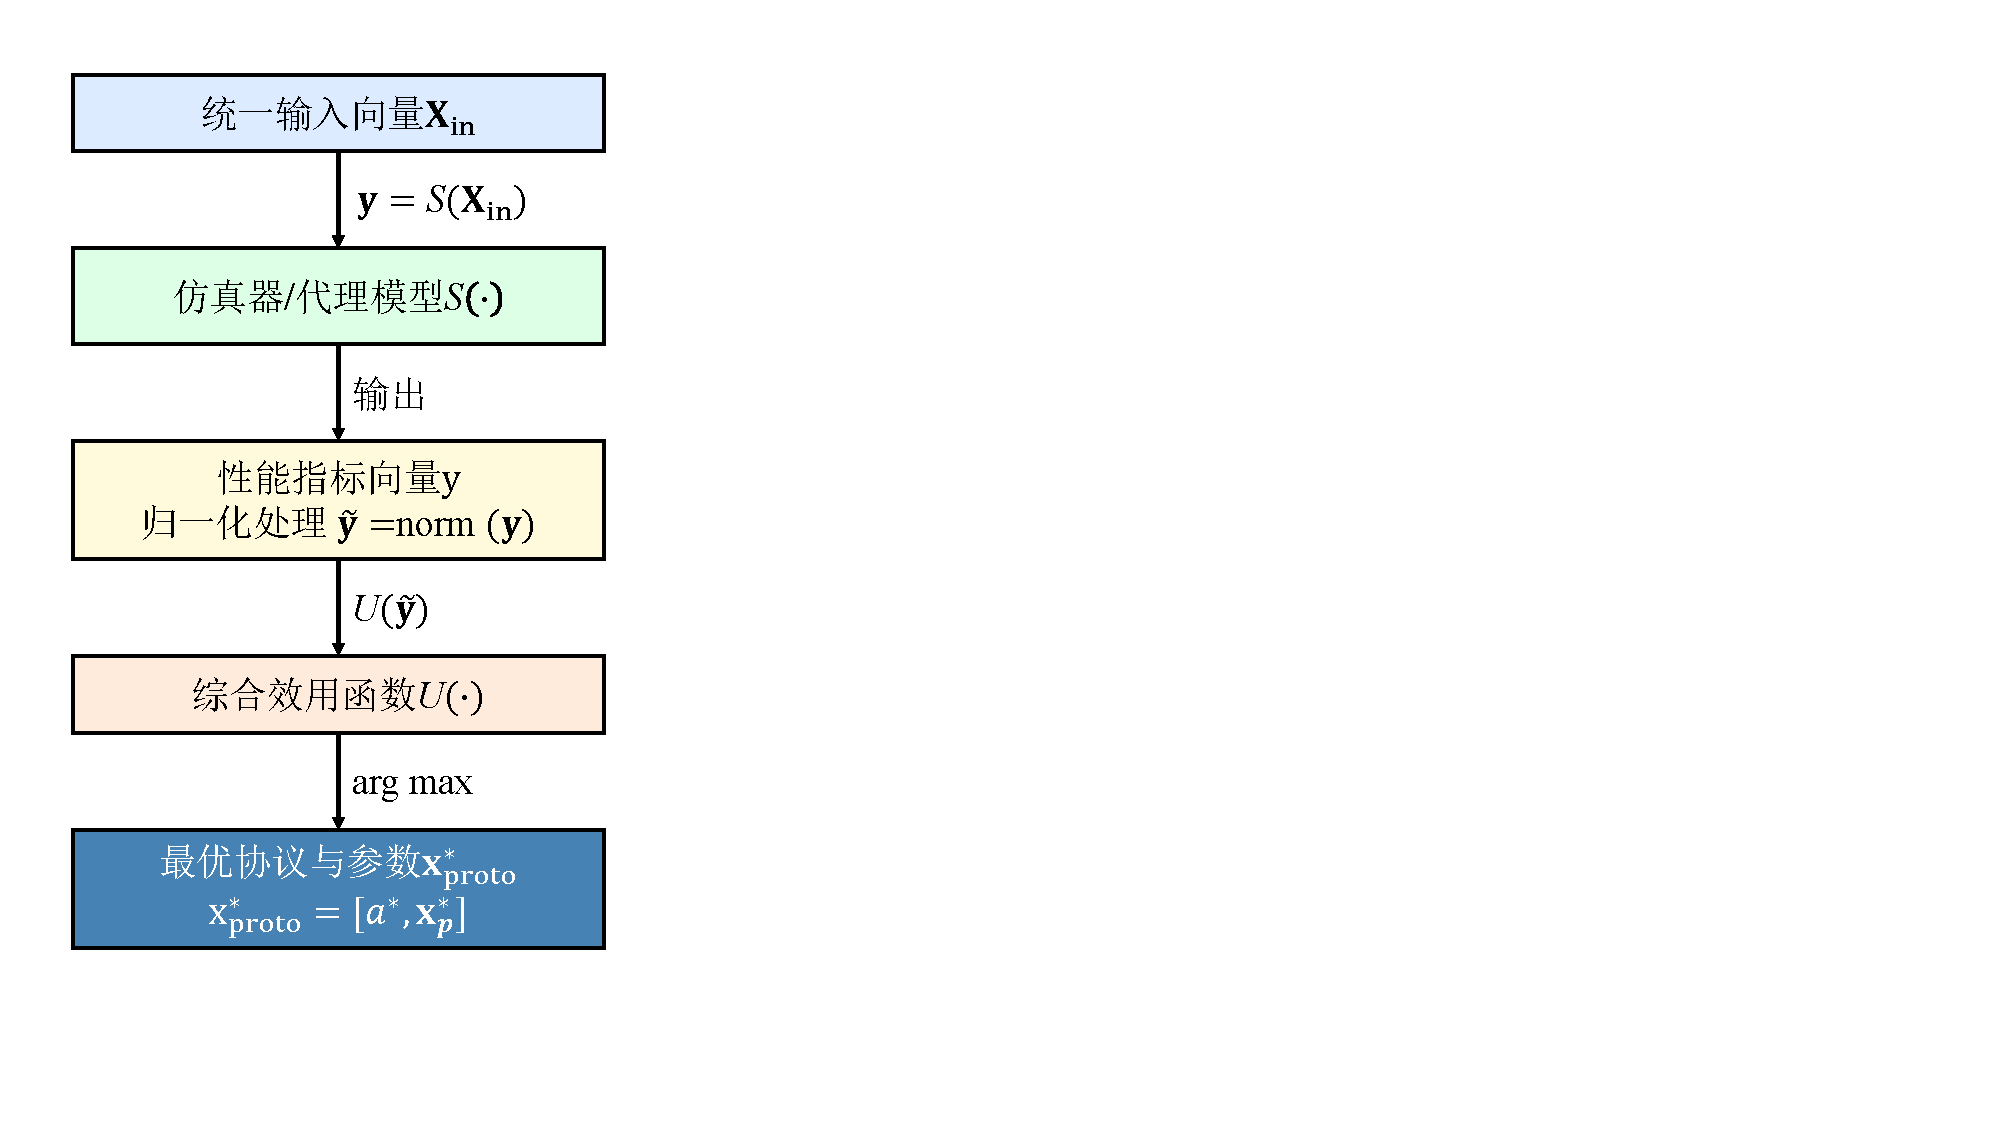
\includegraphics[width=0.95\textwidth]{figure/chap5/model1.pdf}
\caption{统一接入框架与协议选择流程}
\label{fig:chap5_framework}
\end{figure}


\subsection{输入特征标准化与统一接口}
\label{subsec:unified_input}
为实现式~\eqref{eq:chap5_overview} 所需的输入表达，本小节给出统一输入 $\mathbf{X}_{\mathrm{in}}$ 的可实现构造方法。本文将特征划分为三类：通用网络参数 $\mathbf{x}_{\mathrm{common}}$，业务流量特征参数 $\mathbf{x}_{\text{traffic}}$，以及协议专属参数 $\mathbf{x}_{\mathrm{proto}}$ 及其有效性掩码 $\mathbf{m}$。

对于通用网络参数 $\mathbf{x}_{\mathrm{common}}$，将其定义为包含网络规模与仿真配置的向量：
$\mathbf{x}_{\mathrm{common}} = [n,\ T]$,
其中 $n \in \mathbb{N}^+$ 表示网络节点总数，$T \in \mathbb{N}^+$ 表示仿真或观测的时隙总数。上述参数既用于构建仿真场景，也作为后续学习模型的输入特征，共同刻画系统的整体运行条件。

对于业务流量特征 $\mathbf{x}_{\text{traffic}}$，为准确刻画业务到达的多尺度时空统计特性，本文从网络层与节点层两个层级，分别提取负载强度、突发性与周期性三类特征。具体地，定义五维流量特征向量 $\mathbf{x}_{\text{traffic}} = [\hat{\lambda},\ \mathrm{BI}_{\mathrm{net}},\ \mathrm{BI}_{\mathrm{node}},\ \Psi_{\mathrm{net}},\ \Psi_{\mathrm{node}}]$。

设到达矩阵 $\mathbf{A} \in \{0,1\}^{n \times T}$，其中 $A_{i,t}$ 表示节点 $i$ 在时隙 $t$ 是否有包到达。记网络聚合到达序列为 $X(t) = \sum_{i=1}^{n} A_{i,t}$，节点 $i$ 的到达时刻集合为 $\mathcal{T}_i = \{t : A_{i,t} = 1\}$，到达间隔序列为 $\{\Delta t_i^{(k)}\}$，其中 $\Delta t_i^{(k)}$ 为节点 $i$ 第 $k$ 次与第 $k+1$ 次到达的时间间隔。基于此，五维特征定义如下：

\begin{table}[htbp]
\centering
\caption{业务流量特征参数$\mathbf{x}_{\text{traffic}}$的定义与表征含义}
\label{tab:traffic_feature_def}
\renewcommand{\arraystretch}{1.25}
\small
\begin{tabular}{p{2.6cm}|p{1.4cm}|p{6.2cm}|p{4.2cm}}
\toprule
\textbf{名称} & \textbf{变量} & \textbf{计算公式} & \textbf{表征含义} \\
\midrule

归一化网络平均到达率 
& $\hat{\lambda}$ 
& $\hat{\lambda}=\frac{1}{nT}\!\sum_{t=1}^{T}\sum_{i=1}^{n}A_{i,t}$ 
& 表征系统整体流量强度，反映平均活跃节点占比 \\
\hline

网络突发度指标 
& $\mathrm{BI}_{\mathrm{net}}$ 
& $\mathrm{BI}_{\mathrm{net}}
=\frac{\mathrm{ID}_{\mathrm{net}}-1}{\mathrm{ID}_{\mathrm{net}}+1},\;
\mathrm{ID}_{\mathrm{net}}
=\frac{\mathrm{Var}(X(t))}{\mathbb{E}[X(t)]}$ 
& 刻画网络聚合流量的突发性 \\
\hline

节点突发度指标 
& $\mathrm{BI}_{\mathrm{node}}$ 
& $\mathrm{BI}_{\mathrm{node}}
=\frac{\overline{\mathrm{CV}}-1}{\overline{\mathrm{CV}}+1},\;
\overline{\mathrm{CV}}
=\frac{1}{n}\sum_{i=1}^{n}
\frac{\sqrt{\mathrm{Var}(\Delta t_i)}}{\mathbb{E}[\Delta t_i]}$ 
& 刻画单节点到达间隔的突发性 \\
\hline

网络周期性强度 
& $\Psi_{\mathrm{net}}$ 
& $\Psi_{\mathrm{net}}
=\max_{1\le\tau\le\tau_{\max}}
\frac{R(\tau)}{R(0)},
R(\tau)
=\frac{1}{T}\sum_{t=1}^{T-\tau}
\tilde{X}(t)\tilde{X}(t+\tau)$ 
& 网络聚合到达序列的周期性强度 \\
\hline

节点周期性强度 
& $\Psi_{\mathrm{node}}$ 
& $\Psi_{\mathrm{node}}
=\frac{1}{n}\sum_{i=1}^{n}
\max\!\left(0,1-
\frac{\mathrm{Var}(\Delta t_i)}
{(\mathbb{E}[\Delta t_i])^{2}}\right)$ 
& 单节点到达间隔的周期性强度 \\
\bottomrule

\end{tabular}
\end{table}

对于协议专属参数 $\mathbf{x}_{\mathrm{proto}}$，本文采用统一参数超集与掩码的表示方案，以在多协议共存场景下建立统一的输入接口。设候选接入协议集合为 $\mathcal{P} = \{a_1, a_2,  a_3\}$，包括 SA、SAST、CBA协议。每一种协议 $a \in \mathcal{P}$ 对应一组可调参数集合 $\mathcal{X}_p$。
为消除因协议参数维度不一致而产生的维度非对齐问题，本文将候选协议集合中所有参数的并集统一放入一个高维参数向量 $\mathbf{x}_{\mathrm{proto}} \in \mathbb{R}^{d_{\max}}$，其中 $d_{\max} = 1 + \max_{a  \in \mathcal{P}} |\mathcal{X}_p|$ 为统一向量维度，包含协议标识符及所有协议参数的超集。该向量的第一个分量为协议类型标识符 $a \in \mathcal{P}$，其余分量包含接入概率 $q$、连续传输长度 $M$等所有可能的协议参数；当某一协议不涉及其中部分参数时，对应维度仍保留作为占位符。统一参数向量的完整形式为：
$\mathbf{x}_{\mathrm{proto}} = [a, q,\ M, \ldots]$, 
其中省略号对应除列示参数外的其余占位分量。

为严格刻画占位参数在当前协议下的有效性，我们引入与 $\mathbf{x}_{\mathrm{proto}}$ 同维的二值掩码向量 $\mathbf{m} \in \{0,1\}^{d_{\max}}$。在预处理与模型输入阶段，对应掩码为零的参数分量通过元素级乘积 $\mathbf{x}_{\mathrm{proto}} \odot \mathbf{m}$ 被统一置零或屏蔽，从而在保留统一维度表示的同时，防止无效参数对后续学习与优化过程造成干扰。输入特征与性能指标的摘要见表~\ref{tab:input_features}。
完整标准化输入向量表示为
\begin{equation}
\mathbf{X}_{\mathrm{in}} = \big[\mathbf{x}_{\text{traffic}},\ \mathbf{x}_{\mathrm{common}},\ \mathbf{x}_{\mathrm{proto}},\ \mathbf{m}\big].
\end{equation}


\begin{table}[t]
	\centering
	\caption{标准化输入与性能指标摘要}
	\label{tab:input_features}
	\renewcommand{\arraystretch}{1.2}
	\begin{tabular}{@{}l | l | p{9cm}@{}}
	\toprule
		特征组 & 符号 & 含义 / 备注 \\
		\midrule
		$\mathbf{x}_{\text{traffic}}$ & $\hat{\lambda}$ & 归一化网络平均到达率，范围 $[0, 1]$。\\
		& $\mathrm{BI}_{\mathrm{net}}$ & 网络突发度指标，范围 $(-1,1)$。\\
		& $\mathrm{BI}_{\mathrm{node}}$ & 节点突发度指标，范围 $(-1,1)$。\\
		& $\Psi_{\mathrm{net}}$ & 网络周期性强度，范围 $[0,1]$。\\
		& $\Psi_{\mathrm{node}}$ & 节点周期性强度，范围 $[0,1]$。\\
		\midrule
		$\mathbf{x}_{\mathrm{common}}$ & $n$ & 节点数量。\\
		& $T$ & 时隙数量。\\
		\midrule
		$\mathbf{x}_{\mathrm{proto}}$ & $a$ & 协议类型标识，$a\in\mathcal{P}$（向量第一个分量）。\\
		& $q$ & 接入概率。\\
		& $M$ & 连续传输长度。\\
		\midrule
		$\mathbf{m}$ & $m_k$ & 有效性掩码：$m_k=1$ 若第 $k$ 个协议参数在当前协议下有效，否则为 $0$。\\
		\midrule
		$\mathbf{y}$ & $\lambda_{\mathrm{out}}$ & 吞吐量。\\
		& $D$ & 平均时延。\\
		& $J_T$ & 公平性。采用 Jain 指数并做归一化。\\
		& $S$ & 信令开销 \\
		\bottomrule
	\end{tabular}
\end{table}

\subsection{统一仿真映射与效用构造}
\label{subsec:sim_mapping_utility}

在统一输入接口 $\mathbf{X}_{\mathrm{in}}$ 确定后，需要进一步给出从输入到性能度量的可复现映射。为此，本文构建统一的离散事件仿真映射$S(\cdot)$，输入为统一输入向量 $\mathbf{X}_{\mathrm{in}}$，仿真器据此生成对应网络场景并执行随机接入过程，最终输出性能—资源指标向量
\begin{equation}
	\mathbf{y}=S\!\left(\mathbf{X}_{\mathrm{in}}\right)
	=\big[\lambda_{\mathrm{out}},\ D,\ J_T,\ S,\big],
\end{equation}
其中 $\lambda_{\mathrm{out}}$ 表示系统吞吐量，$D$ 表示平均数据包时延，$J_T$ 表示公平性（采用 Jain 指数刻画），$S$ 表示信令开销。上述指标集合兼顾业务性能与代价，便于在多协议、多参数配置下进行统一评估与对比。
为消除不同指标量纲与数值尺度差异对比较与决策造成的影响，并保证跨协议评估的一致性，本文在同一对比组内对各维指标采用最小最大归一化，并将所有指标统一转换为效用型指标。记第 $k$ 个指标 $y_k$ 在对比组内的取值范围为 $[y_k^{\min}, y_k^{\max}]$，则归一化后的指标 $\tilde{y}_k$ 定义为
\begin{equation}
	\tilde{y}_k =
	\begin{cases}
	\dfrac{y_k-y_k^{\min}}{y_k^{\max}-y_k^{\min}}, & y_k \ \text{为效用型指标},\\[10pt]
	1-\dfrac{y_k-y_k^{\min}}{y_k^{\max}-y_k^{\min}}, & y_k \ \text{为成本型指标},
	\end{cases}
\end{equation}
其中效用型指标是指数值增大表示性能提升的指标，如吞吐量 $\lambda_{\mathrm{out}}$ 和公平性 $J_T$；成本型指标是指数值减小表示性能改善的指标，如时延 $D$ 与信令开销 $S$。该归一化方法将所有指标映射至 $[0,1]$ 区间，并保证归一化后的指标均满足数值越大性能越优的单调关系。由此得到归一化指标向量
\begin{equation}
	\tilde{\mathbf{y}}=\mathrm{norm}(\mathbf{y})
	=\big[\tilde{\lambda}_{\mathrm{out}},\ \tilde{D},\ \tilde{J}_T,\ \tilde{S}\big].
\end{equation}

在此基础上，为将多维指标映射为单一可优化目标，本文采用加权线性效用函数
\begin{equation}
	U\big(\tilde{\mathbf{y}}\big)=
	w_{\lambda}\tilde{\lambda}_{\mathrm{out}}
	+w_{D}\tilde{D}
	+w_{J}\tilde{J}_T
	+w_{S}\tilde{S},
\end{equation}
其中 $w_i\ge 0$ 且 $\sum_i w_i=1$。权重向量 $\{w_i\}$ 用于表征业务对吞吐、时延、公平性以及信令开销的偏好，可依据应用需求设定；同时，可通过改变权重进行敏感性分析，以检验联合选择结论的稳健性。

\subsection{等价资源约束下的联合优化问题}
\label{subsec:equiv_constrained_opt}
为便于后续性能预测模型训练与快速优化算法中目标计算、约束检查与可行域投影的统一实现，本节将式~\eqref{eq:chap5_overview} 所述问题改写为标准约束优化形式。该表述与原问题在决策变量、优化目标及约束条件上完全等价，区别仅在于将隐式关系显式展开，以适配标准优化求解器的输入要求。

优化问题的标准形式表述如下：
\begin{equation}\label{eq:chap5_constrained}
	\begin{aligned}
		\max_{\,\mathbf{x}_{\mathrm{proto}}\in\mathcal{X}} \quad 
		& U\big( \tilde{\mathbf{y}} \big) \\[6pt]
		\text{s.t.}\quad
		& \mathbf{X}_{\mathrm{in}}=\big[\mathbf{x}_{\text{traffic}},\ \mathbf{x}_{\mathrm{common}},\ \mathbf{x}_{\mathrm{proto}},\ \mathbf{m}\big],\\[3pt]
		& \tilde{\mathbf{y}} = \mathrm{norm}\!\left(\mathbf{y}\right),\ \mathbf{y} = S\!\left( \mathbf{X}_{\mathrm{in}} \right), \\[4pt]
		& S\big(\mathbf{x}_{\mathrm{proto}}\big) \le S_{\max}.
	\end{aligned}
\end{equation}
式~\eqref{eq:chap5_constrained} 的决策变量为统一参数向量 $\mathbf{x}_{\mathrm{proto}}$，其第一个分量 $\mathbf{x}_{\mathrm{proto}}[1]$ 为协议标识符，其余分量为各协议参数。决策变量需满足所选协议的合法参数空间约束，通过掩码 $\mathbf{m}$ 界定有效参数维度。第一行约束显式构建统一输入向量，第二行约束定义从输入到归一化性能指标的映射关系。第三行约束限定信令开销不超过系统资源阈值 $S_{\max}$。
可以看到，该优化问题的解为满足全部约束的最优统一参数向量 $\mathbf{x}_{\mathrm{proto}}^*$，其中包含了最优协议类型及其对应参数。


% =========================================================
% 第 5.2 节：仿真数据生成与性能分析
% =========================================================

\section{基于离散事件仿真的接入协议数据集构建与仿真结果分析}
\label{sec:simulation_data}

为训练能够准确预测不同协议配置下网络性能的模型，需要构建高质量的训练数据集。本节首先阐述参数空间的采样策略，随后在\ref{subsec:unified_simulator}小节介绍统一仿真器 $S(\cdot)$ 的设计与实现，接着详细说明基于仿真器的数据集生成流程，最后通过可视化分析展示不同协议在典型场景下的性能差异，为后续性能预测模型的构建提供数据基础与性能基准。

\subsection{两阶段参数空间采样策略}
\label{subsec:grid_sampling}

训练数据质量取决于参数空间覆盖与关键区域分辨率。为兼顾两者，本文在混合空间 $\{\mathbf{x}_{\text{traffic}},\mathbf{x}_{\mathrm{proto}}\}$ 上采用“两阶段采样”策略：第一阶段做全局粗采样，第二阶段做峰值与转折区细采样。采样维度分为流量强度 $\hat{\lambda}$、流量形态、协议参数三类，其中流量形态在两个阶段均固定为三类场景并保持一致遍历，以保证跨协议、跨阶段结果可比。图~\ref{fig:dataset_sampling_strategy} 给出流程示意。

\begin{figure}[t]
	\centering
	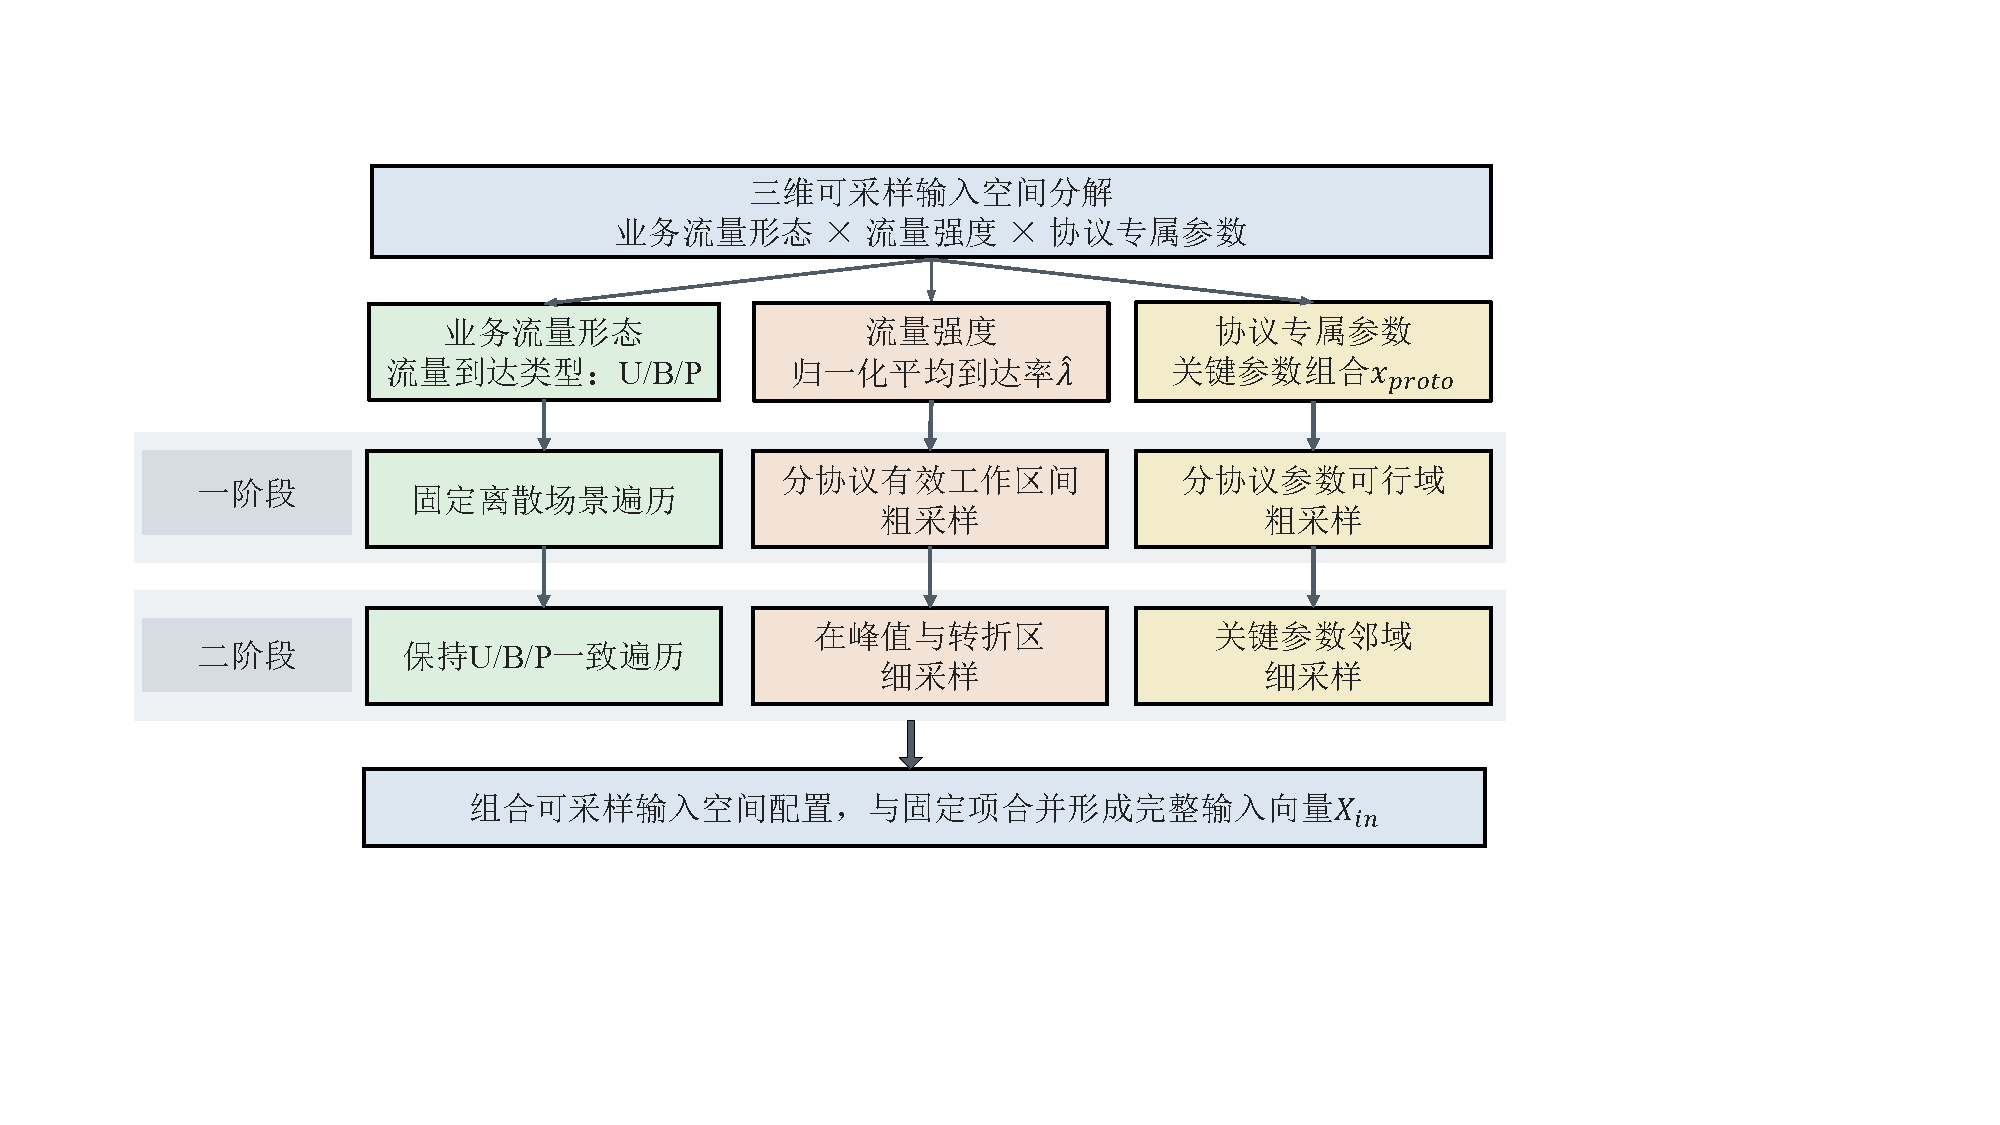
\includegraphics[width=0.99\textwidth]{figure/chap5/数据集采样策略.pdf}
	\caption{两阶段参数空间采样策略流程图}
	\label{fig:dataset_sampling_strategy}
\end{figure}
流量形态维度采用三类离散场景：均匀到达（U）、突发到达（B）、周期到达（P）。在第一阶段与第二阶段中，任一 $\hat{\lambda}$ 与任一协议参数组合都必须在 U/B/P 三类流量下分别仿真一次，确保每阶段数据集都包含三类流量样本。

% 其流量特征为 $\mathrm{BI}_{\mathrm{net}} \approx 0$ 且 $\Psi_{\mathrm{net}} \approx 0$，对应近似泊松到达过程。
% 其流量特征为 $\mathrm{BI}_{\mathrm{net}} \in [0.3, 0.7]$ 且 $\Psi_{\mathrm{net}} \in [0, 0.2]$，表征中等至强突发性。
% 其流量特征为 $\mathrm{BI}_{\mathrm{net}} \in [-0.5, -0.2]$ 且 $\Psi_{\mathrm{net}} \in [0.6, 0.9]$，体现规则周期结构。

第一阶段为粗粒度均匀采样，其目标是在较低计算成本下获取各协议性能曲线的全局轮廓。核心原则是按协议有效工作区间设置差异化 $\hat{\lambda}$ 采样范围，而非统一范围。
具体而言，SA 的理论最大吞吐约为 $1/e\approx0.368$，因此其采样点应主要落在 $[0,1/e]$；仅保留少量 $>1/e$ 的样本点用于刻画饱和边界。SAST 的有效高吞吐区通常延伸至约 0.5，采样上限应相应提高。CBA 在较高负载下仍可能保持较好吞吐，其上限可进一步放宽，但仍以可工作区间为准，避免无效超载样本。
对于每个粗采样点，均在 U/B/P 三类流量下生成样本，从而可在相同平均到达率下直接比较不同流量形态对协议性能的影响。
协议参数亦采用针对各协议的专属粗采样：连续参数（如 $q$）作稀疏均匀取点，离散参数（如 $M$）遍历典型可行值，二者的笛卡尔积构成第一阶段配置集合。综上，第一阶段样本由协议类型、流量强度粗网格、协议参数粗网格与三类流量形态共同组成。基于该阶段结果，可进一步定位各协议在不同流量形态下的峰值区与性能转折区。

第二阶段为峰值及转折区域细采样，从而进一步提高采样分辨率。具体实现方法为：根据第一阶段结果，为每种协议在每类流量形态下确定峰值区间与转折区间，在该区间内以更小步长对 $q$ 进行局部加密采样，以提升最优工作点邻域的采样分辨率。第二阶段的样本量根据各协议关键区间的宽度自适应确定。
最终将两阶段样本合并形成训练集：第一阶段保证全局覆盖，第二阶段强化关键区域。与全空间均匀细采样相比，该策略在控制样本规模的同时提高了最优工作点附近的建模精度。

% 为便于后续统一补充实验数据，表~\ref{tab:two_stage_sampling_template} 给出两阶段采样配置总表模板。

% \begin{table}[htbp]
% \centering
% \caption{两阶段采样配置总表（模板，待补充）}
% \label{tab:two_stage_sampling_template}
% \renewcommand{\arraystretch}{1.2}
% \setlength{\tabcolsep}{3pt}
% \small
% \begin{tabular}{p{0.9cm} p{1.0cm} p{1.3cm} p{2.2cm} p{1.0cm} p{3.2cm} p{3.0cm}}
% \toprule
% 协议 & 阶段 & 流量形态 & $\hat{\lambda}$采样区间 & 步长 & 协议参数采样设置 & 样本统计（单形态/三形态/有效） \\
% \midrule
% SA & 粗采样 & U/B/P & [\ ,\ ] & [\ ] & $q:\,$[\ ] & [\ ] / [\ ] / [\ ] \\
% SA & 细采样 & U/B/P & [\ ,\ ] & [\ ] & $q:\,$[\ ] & [\ ] / [\ ] / [\ ] \\
% SAST & 粗采样 & U/B/P & [\ ,\ ] & [\ ] & $q:\,$[\ ] & [\ ] / [\ ] / [\ ] \\
% SAST & 细采样 & U/B/P & [\ ,\ ] & [\ ] & $q:\,$[\ ] & [\ ] / [\ ] / [\ ] \\
% CBA & 粗采样 & U/B/P & [\ ,\ ] & [\ ] & $q:\,$[\ ], $M:\,$[\ ] & [\ ] / [\ ] / [\ ] \\
% CBA & 细采样 & U/B/P & [\ ,\ ] & [\ ] & $q:\,$[\ ], $M:\,$[\ ] & [\ ] / [\ ] / [\ ] \\
% \midrule
% \multicolumn{6}{r}{总计} & [\ ] / [\ ] / [\ ] \\
% \bottomrule
% \end{tabular}
% \end{table}



\subsection{统一仿真器的设计与实现}
\label{subsec:unified_simulator}

统一仿真器 $S(\cdot)$ 是连接输入配置与性能指标的核心映射模块，其设计需同时满足多协议支持、精确性与可扩展性要求。本文基于离散事件仿真框架采用模块化设计实现该仿真器，通过各模块的协调完成对三种随机接入协议的统一建模与性能评估。
统一仿真器采用分层模块化架构，包含以下核心组件：

\begin{itemize}[leftmargin=*]
	\item \textbf{配置解析模块}：解析统一输入向量 $\mathbf{X}_{\mathrm{in}}$，提取网络参数 $\mathbf{x}_{\text{common}}$、流量特征向量 $\mathbf{x}_{\text{traffic}}$ 以及协议专属参数向量 $\mathbf{x}_{\mathrm{proto}}$。其中 $\mathbf{x}_{\text{traffic}}$ 的可配置项为归一化平均到达率 $\hat{\lambda}$。此外，还需单独指定流量类型标识 $\text{traffic\_type}$ 以确定流量生成模型。

	\item \textbf{流量生成与特征提取模块}：依据流量类型标识 $\text{traffic\_type}$ 选择相应的到达过程模型，即均匀到达采用泊松过程、突发到达采用马尔可夫调制泊松过程、周期到达采用确定性周期同步过程，各类型模型的内部生成参数均预先设定。在给定归一化平均到达率 $\hat{\lambda}$ 下，为各节点按时隙生成到达包序列。由于生成参数固定，所得流量序列仅覆盖有限组预定义的突发强度与周期强度，从而保证不同实验配置间的可复现性。在此基础上，基于生成的到达包序列计算并输出 $\mathbf{x}_{\text{traffic}}$ 中除 $\hat{\lambda}$ 外的特征指标 $\mathrm{BI}_{\mathrm{net}}$、$\mathrm{BI}_{\mathrm{node}}$、$\Psi_{\mathrm{net}}$ 与 $\Psi_{\mathrm{node}}$。

	\item \textbf{协议执行与仿真模块}：协议策略由协议专属参数向量 $\mathbf{x}_{\mathrm{proto}}$ 参数化，其首个分量为协议类型标识 $a$，其余分量为对应协议的参数配置。仿真器在运行前根据协议标识 $a$ 加载相应的协议执行引擎，并在每个时隙依据参数策略完成发送决策与队列状态更新，同时与信道仿真子模块协同完成并行发送的冲突检测。各协议的核心接入机制封装如下：
	\begin{itemize}[leftmargin=*, itemsep=0.2em]
		\item \textbf{SA}：时隙Aloha协议，节点有数据包时以固定接入概率 $q$ 尝试发送。
		\item \textbf{SAST}：连续传输时隙Aloha协议，当上一时隙发送成功时接入概率置1并连续传输，否则恢复以概率 $q$ 随机接入。
		\item \textbf{CBA}：基于连接的Aloha协议，当节点缓存队列中数据包数量不小于 $M$ 时，以概率 $q$ 尝试建立连接，连接建立成功后无竞争地连续发送 $M$ 个数据包。
	\end{itemize}

	\item \textbf{性能统计模块}：实时记录成功发送包数、累计时延、各节点吞吐、信令开销等统计量，在仿真完成后计算最终的吞吐量 $\lambda_{\mathrm{out}}$、平均时延 $D$、公平性指数 $J_T$、信令开销 $S$。
\end{itemize}

上述模块通过统一接口在离散事件仿真框架下协同运行，从而实现对多协议、多参数配置的统一评估。仿真器的整体执行流程遵循初始化、时隙迭代与结果汇总三个阶段，如图~\ref{fig:unified_simulator_main} 所示。
\begin{figure}[t]
\centering
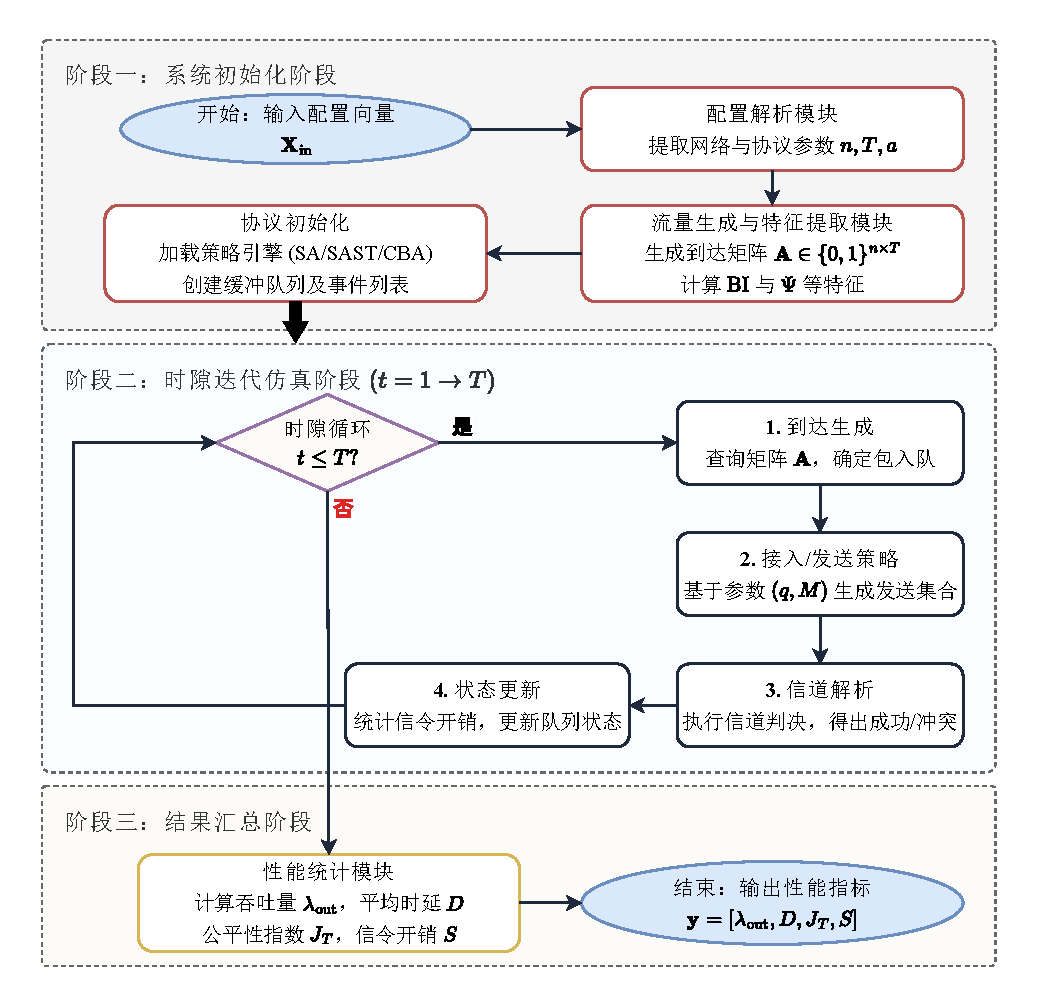
\includegraphics[width=0.95\textwidth]{figure/chap5/仿真器实现流程框图.pdf}
\caption{统一仿真器设计与实现流程图}
\label{fig:unified_simulator_main}
\end{figure}



% \begin{algorithm}[htbp]
% 	\caption{统一仿真器执行流程}
% 	\label{alg:unified_simulator_main}
% 	\KwIn{配置参数 $\mathbf{X}_{\text{in}} = (\mathbf{x}_{\mathrm{common}}, \mathbf{x}_{\text{traffic}}, \mathbf{x}_{\mathrm{proto}}, \mathbf{m})$, \text{traffic\_type} }
% 	\KwOut{性能指标 $\mathbf{y} = [\lambda_{\mathrm{out}}, D, J_T, S]$}
	
% 	配置解析模块：$n, T, \text{traffic\_type}, \hat{\lambda}, \mathbf{x}_{\mathrm{proto}} \leftarrow \text{Parse}(\mathbf{X}_{\text{in}})$\\
% 	协议标识提取：$a \leftarrow \mathbf{x}_{\mathrm{proto}}[1]$\\
% 	系统初始化：创建 $n$ 个节点的缓冲队列、信道状态记录、事件队列\\
% 	流量生成与特征提取：基于 $\text{traffic\_type}$ 和归一化网络平均到达率 $\hat{\lambda}$ 选择到达过程（参数预设），生成到达矩阵 $\mathbf{A}\in\{0,1\}^{n\times T}$，并计算更新 $\mathrm{BI}_{\mathrm{net}}$、$\mathrm{BI}_{\mathrm{node}}$、$\Psi_{\mathrm{net}}$、$\Psi_{\mathrm{node}}$\\
% 	加载协议引擎以及参数：根据$a$加载协议执行引擎，根据$\mathbf{x}_{\mathrm{proto}}$加载协议策略\\

% 	性能统计初始化：$\text{success\_counter} \leftarrow 0, \text{delay\_counter} \leftarrow 0, \text{signaling\_cost} \leftarrow 0$\\
% 	\For{$t = 1$ \textbf{to} $T$}{
% 		1. 到达生成：由到达矩阵$\mathbf{A}\in\{0,1\}^{n\times T}$确定各节点的包入队情况\;
		
% 		2. 接入/发送策略：根据协议规则与协议参数生成发送集合\;
		
% 		3. 信道解析：执行信道判决，得到并行发送导致的成功/冲突结果\;
		
% 		4. 统计信令开销：根据协议机制统计本时隙信令相关操作（如连接建立、预约、反馈等）\;
		
% 		5. 根据成功结果更新队列/协议内部状态，并更新统计量\;
% 	}
% 	计算吞吐量：$\lambda_{\mathrm{out}} \leftarrow \text{success\_counter} / T$\\
% 	计算平均时延：$D \leftarrow \text{sum\_delay} / \text{success\_counter}$\\
% 	计算公平性指数：$J_T \leftarrow \text{Jain}(\text{node\_throughputs})$\\
% 	计算信令开销：$S \leftarrow \text{sum\_signaling\_cost} / T$\\
% 	组织输出：$\mathbf{y} \leftarrow [\lambda_{\mathrm{out}}, D, J_T, S]$\\
% 	\Return $\mathbf{y}$
% \end{algorithm}

% 通过上述设计，统一仿真器能够高效、准确地评估不同协议配置下的网络性能，为数据集构建提供可靠的性能标签。仿真配置与数据统计信息在表~\ref{tab:dataset_summary}中统一汇总。

\subsection{数据集构建与预处理}
\label{subsec:dataset_construction}

基于两阶段采样策略与统一仿真器，本文构建了覆盖三种协议、多种流量强度与参数配置的综合性能数据集。数据集构建过程如下：
\begin{enumerate}[leftmargin=*]
	\item \textbf{采样执行}：针对候选协议集合 $\mathcal{P} = \{\text{SA, SAST, CBA}\}$，依照前述网格搜索策略生成参数组合。各采样变量与仿真器关键参数一一对应，主要参数与统计结果统一汇总于表~\ref{tab:dataset_summary}。以SA协议为例，主要参数包括归一化网络平均到达率$\hat{\lambda}$和接入概率 $q$，分别在设定区间内均匀采样，最终形成多组参数配置。

	\item \textbf{仿真执行}：对每组参数配置，调用统一仿真器开展仿真实验。仿真器在固定网络规模与仿真时隙数下运行并输出各项性能指标。为降低随机性影响，每组配置重复进行多次独立实验，以各项性能指标的均值作为该配置的性能标签。

	\item \textbf{数据清洗}：对仿真结果进行筛查，剔除仿真失败或出现异常值的样本，并对极端异常值进行标记。清洗后保留有效样本，并保留可用于协议比较的完整标签记录。

	\item \textbf{归一化处理}：对连续型特征保持在定义域内，流量特征已在特征提取阶段归一化至特定区间。离散型特征采用适当的编码方式。性能指标采用最小最大归一化处理，以提升后续模型训练的效率和稳定性。

	\item \textbf{数据划分}：将数据集划分为训练集、验证集和测试集。为保证协议类型在各子集中分布均衡，采用分层随机划分策略，确保数据划分的科学性和代表性。
\end{enumerate}


\begin{table}[t]
\centering
\caption{仿真数据集关键配置与统计信息}
\label{tab:dataset_summary}
\renewcommand{\arraystretch}{1.25}
\setlength{\tabcolsep}{5.5pt}
\small
\begin{tabular}{@{}p{2.7cm} p{6cm} p{6.5cm}@{}}
\toprule
\textbf{类别} & \textbf{参数范围 / 统计值} & \textbf{说明} \\
\midrule

\multicolumn{3}{c}{\textit{数据集规模（Dataset Overview）}} \\

样本总数 
& 16940 
& 离散事件仿真生成的有效样本总数。 \\

输入特征结构 
& 28 个数值特征 + 2 个类别特征 
& 包括协议参数、流量特征等。 \\

% 特征覆盖率 
% & 平均覆盖率 $95.8\%$ 
% & 大部分字段在所有样本中均存在，部分 CBA 参数仅在对应协议下生效。 \\

\midrule
\multicolumn{3}{c}{\textit{协议配置空间（Protocol Space）}} \\

候选协议集合 
& $\mathcal{P}=\{\mathrm{SA},\mathrm{SAST},\mathrm{CBA}\}$ 
& 分别表示三种协议。 \\

发送概率参数 
& $q\in[0,0.02]$ \quad (mean $0.00756$) 
& 协议发送概率或接入控制参数。 \\

CBA协议参数 
& $M\in\{1,2,4\}$,\quad $\delta=1$ 
& $M$为连续传输数据包，$\delta$为信令的时间开销，仅在该协议下启用。 \\

\midrule
\multicolumn{3}{c}{\textit{流量配置空间（Traffic Space）}} \\

流量类型 
& $\{U,B,P\}$ 
& 分别表示均匀流量（Uniform）、突发流量（Bursty）和周期流量（Periodic）。 \\

归一化到达率 
& $\hat{\lambda}\in\{0.1,0.3,0.5,1\}$ \quad (mean $0.00475$) 
& 网络整体到达强度。 \\


流量特征 
& $\Psi_{\text{net}}\in[0.0026,0.9997]$ 
& 描述网络层流量突发性。 \\

\midrule
\multicolumn{3}{c}{\textit{仿真环境配置（Simulation Settings）}} \\

节点数量 
& $n=100$ 
& 网络中竞争随机接入的终端节点数量。 \\

仿真时隙长度 
& $T=3\times10^{5}$ 
& 每次仿真运行的总时隙数。 \\

样本索引范围 
& $[0,16939]$ 
& 数据集样本编号范围。 \\

\midrule
\multicolumn{3}{c}{\textit{输出标签统计（Output Labels）}} \\

系统吞吐量 
& $\lambda_{\mathrm{out}}\in[0,0.520]$ \quad (mean $0.218$) 
&  \\


公平性指标 
& $J_T\in[0,1)$ \quad (mean $0.9796$) 
&  \\

平均时延 
& $D\in[0,1.62\times10^{5}]$ \quad (mean $5.72\times10^{4}$) 
&  \\

信令开销 
& $S\in[0,5.546]$ \quad (mean $1.158$) 
&  \\

\midrule
\multicolumn{3}{c}{\textit{归一化标签（Learning Targets）}} \\

归一化时延 
& $\tilde{D}\in[0,1]$ \quad (mean $0.502$) 
&归一化后的时延指标。 \\

% 归一化公平性 
% & $\tilde{J}_T\in[0,1]$ \quad (mean $0.980$) 
% & 归一化后的公平性指标。 \\

归一化信令开销 
& $\tilde{S}\in[0,1]$ \quad (mean $0.613$) 
& 归一化后的信令开销指标。 \\

\bottomrule
\end{tabular}
\end{table}
表~\ref{tab:dataset_summary}汇总了数据集中与实验可复现性相关的关键配置，包括仿真环境设置、协议参数空间及主要输出标签的统计范围。基于上述流程，本文构建了一个覆盖多协议、多参数配置及多类流量形态的仿真数据集。所有标签均由统一仿真器在一致的网络规模与统计口径下生成，保证了数据的可比性与可复现性。该数据集既可用于后续性能预测模型的训练与验证，也为不同随机接入协议的性能对比提供统一的数据基础。


% \subsection{仿真性能验证与对比}
% \label{subsec:protocol_performance_comparison}
% 为在性能预测模型训练之前建立可复现的性能基准，并验证多协议共存框架的必要性，本小节直接基于\ref{subsec:dataset_construction}节构建的数据集开展对比分析。具体而言，本文将数据集按流量形态与协议类型进行分组，并在每一组内设置参数配置作为对比切片。在保持网络规模、统计口径与标签生成方式一致的条件下，通过绘制吞吐量、时延、公平性与信令开销等指标随归一化网络平均到达率 $\hat{\lambda}$和 传输概率$q$ 变化的曲线，展示不同协议在典型场景下的性能演化规律，从而形成后续性能预测模型训练与预测结果的基准参照。

% \textbf{吞吐量对比。} 
% 图~\ref{fig:protocol_throughput_comparison} 给出了不同协议随 $\hat{\lambda}$ 变化的输出吞吐量 $\lambda_{\mathrm{out}}$ 曲线。
% \begin{figure}[t]
% 	\centering
% 	\subfloat[均匀场景]{
% 		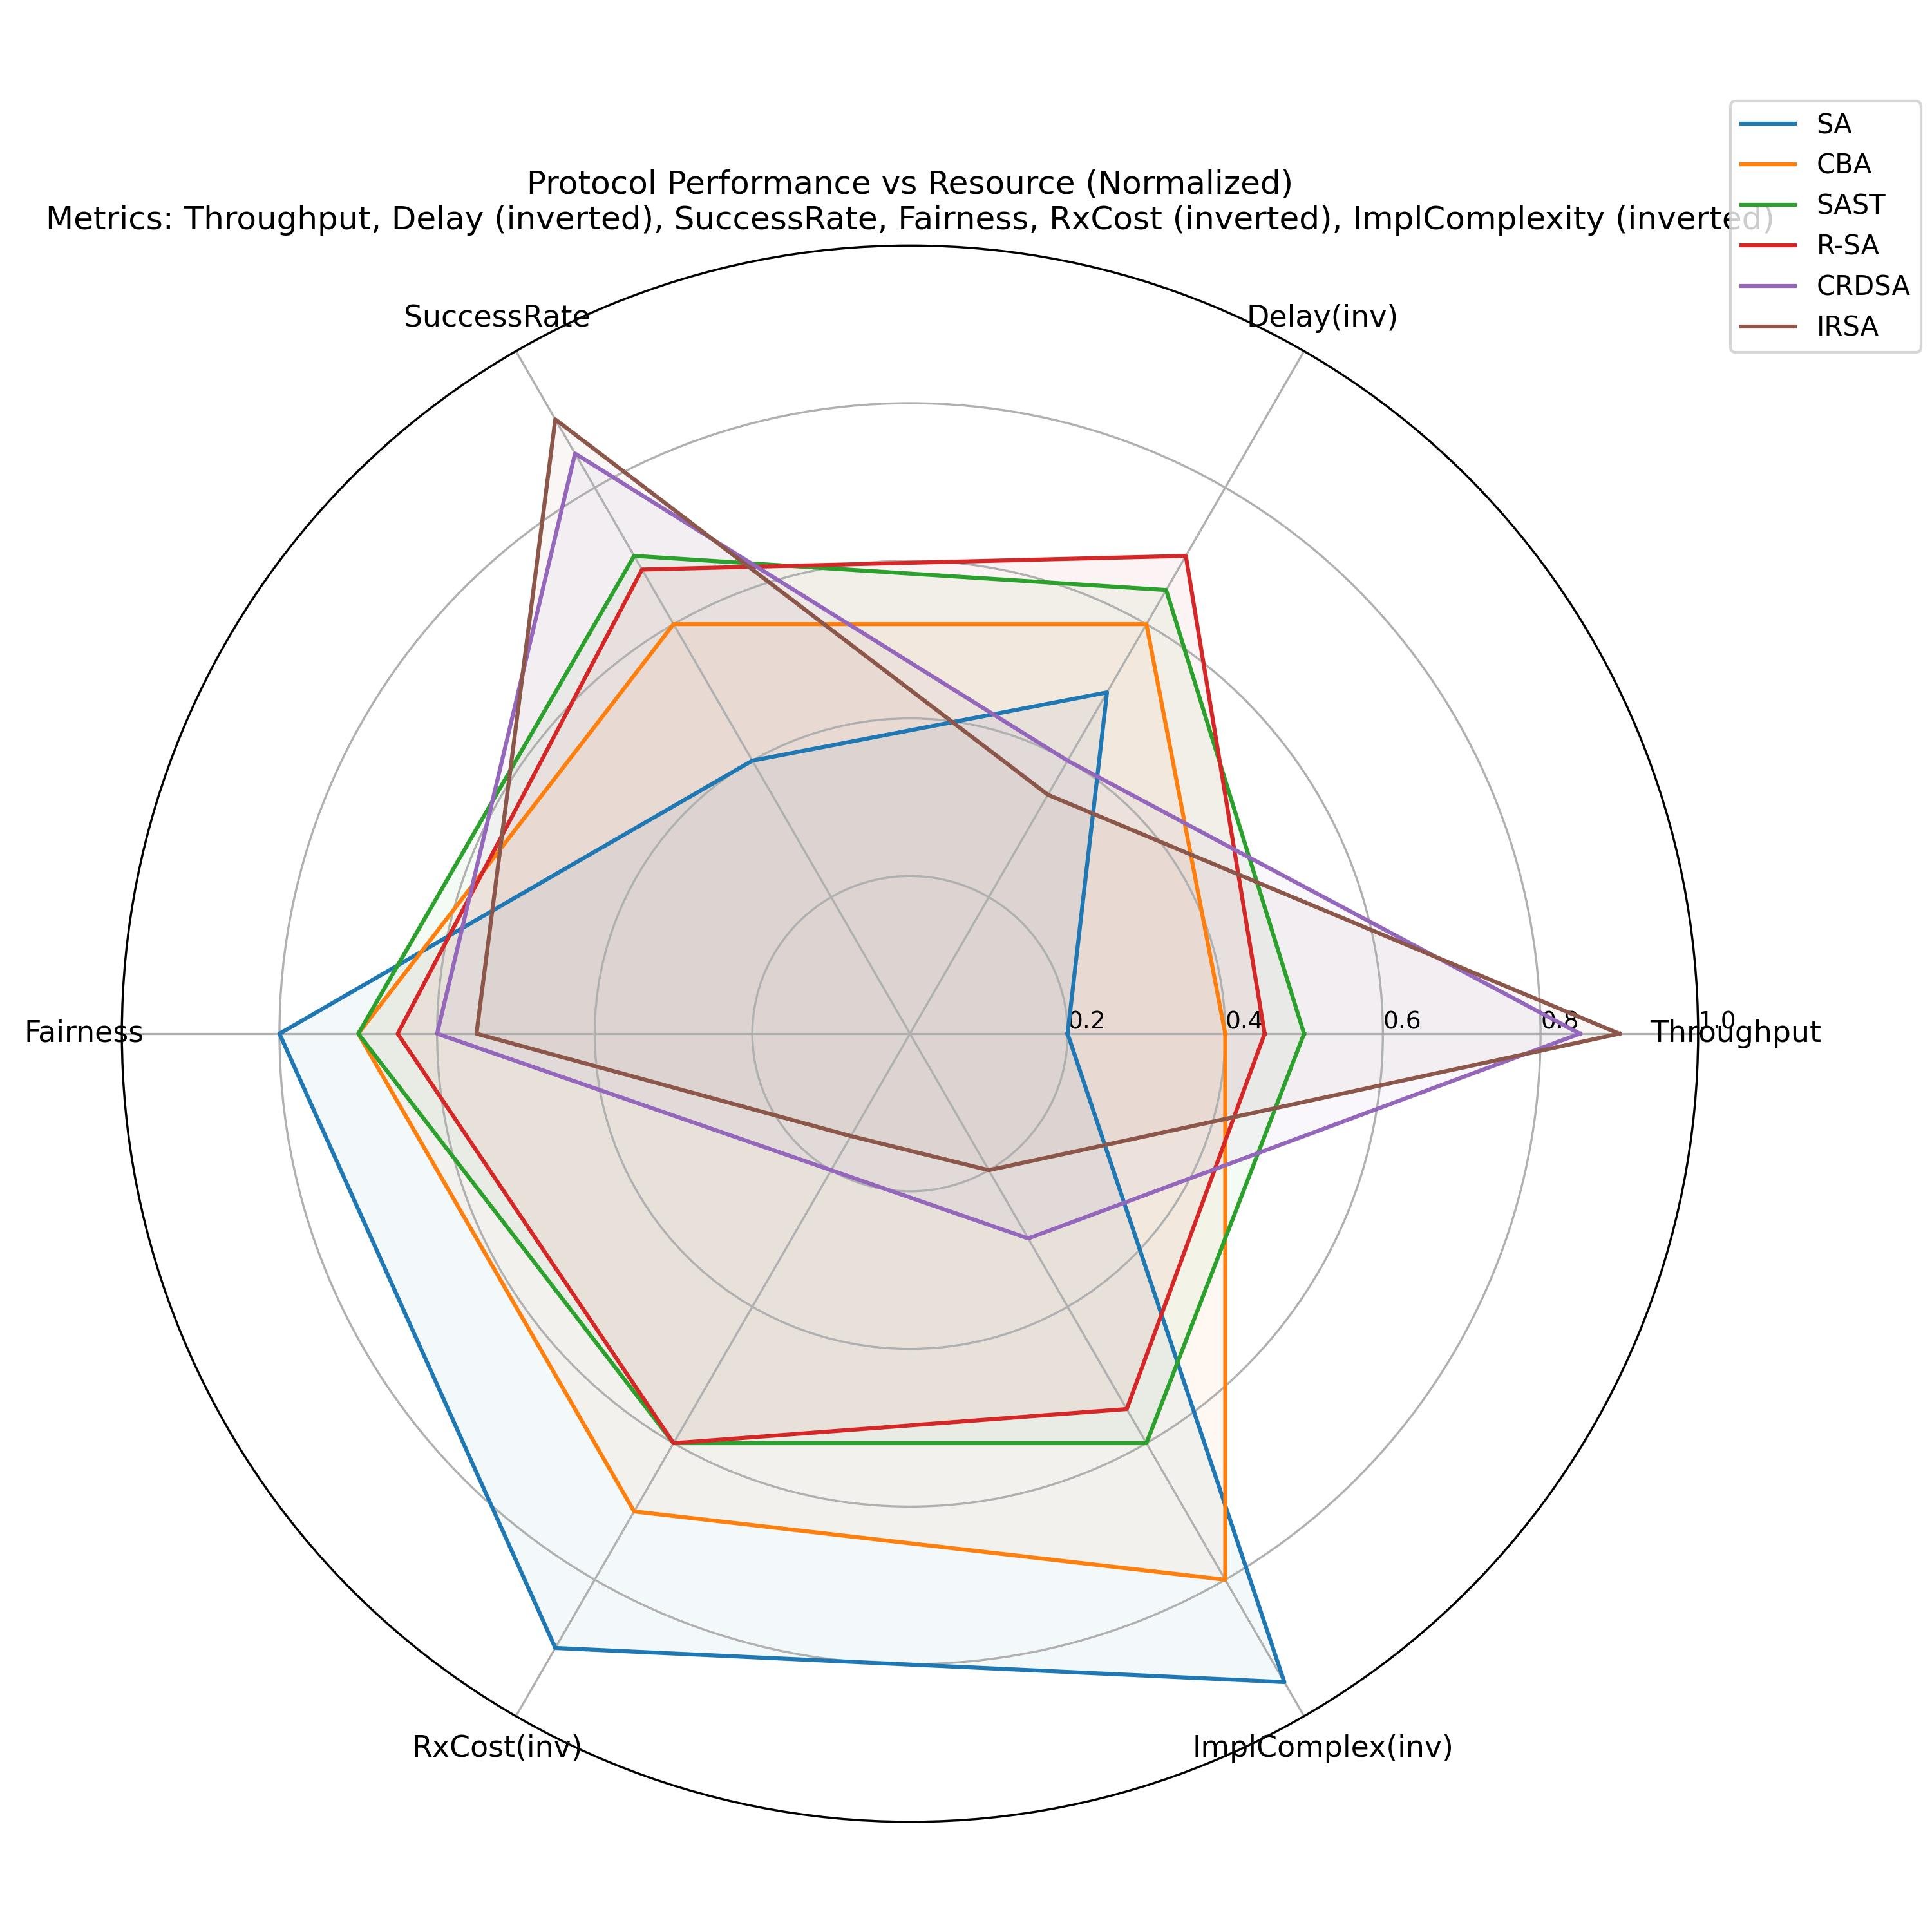
\includegraphics[width=0.3\textwidth]{figure/chap5/Sim11.jpg}
% 		\label{fig:protocol_throughput_comparison1}
% 	}
% 	\hfill
% 	\subfloat[突发场景]{
% 		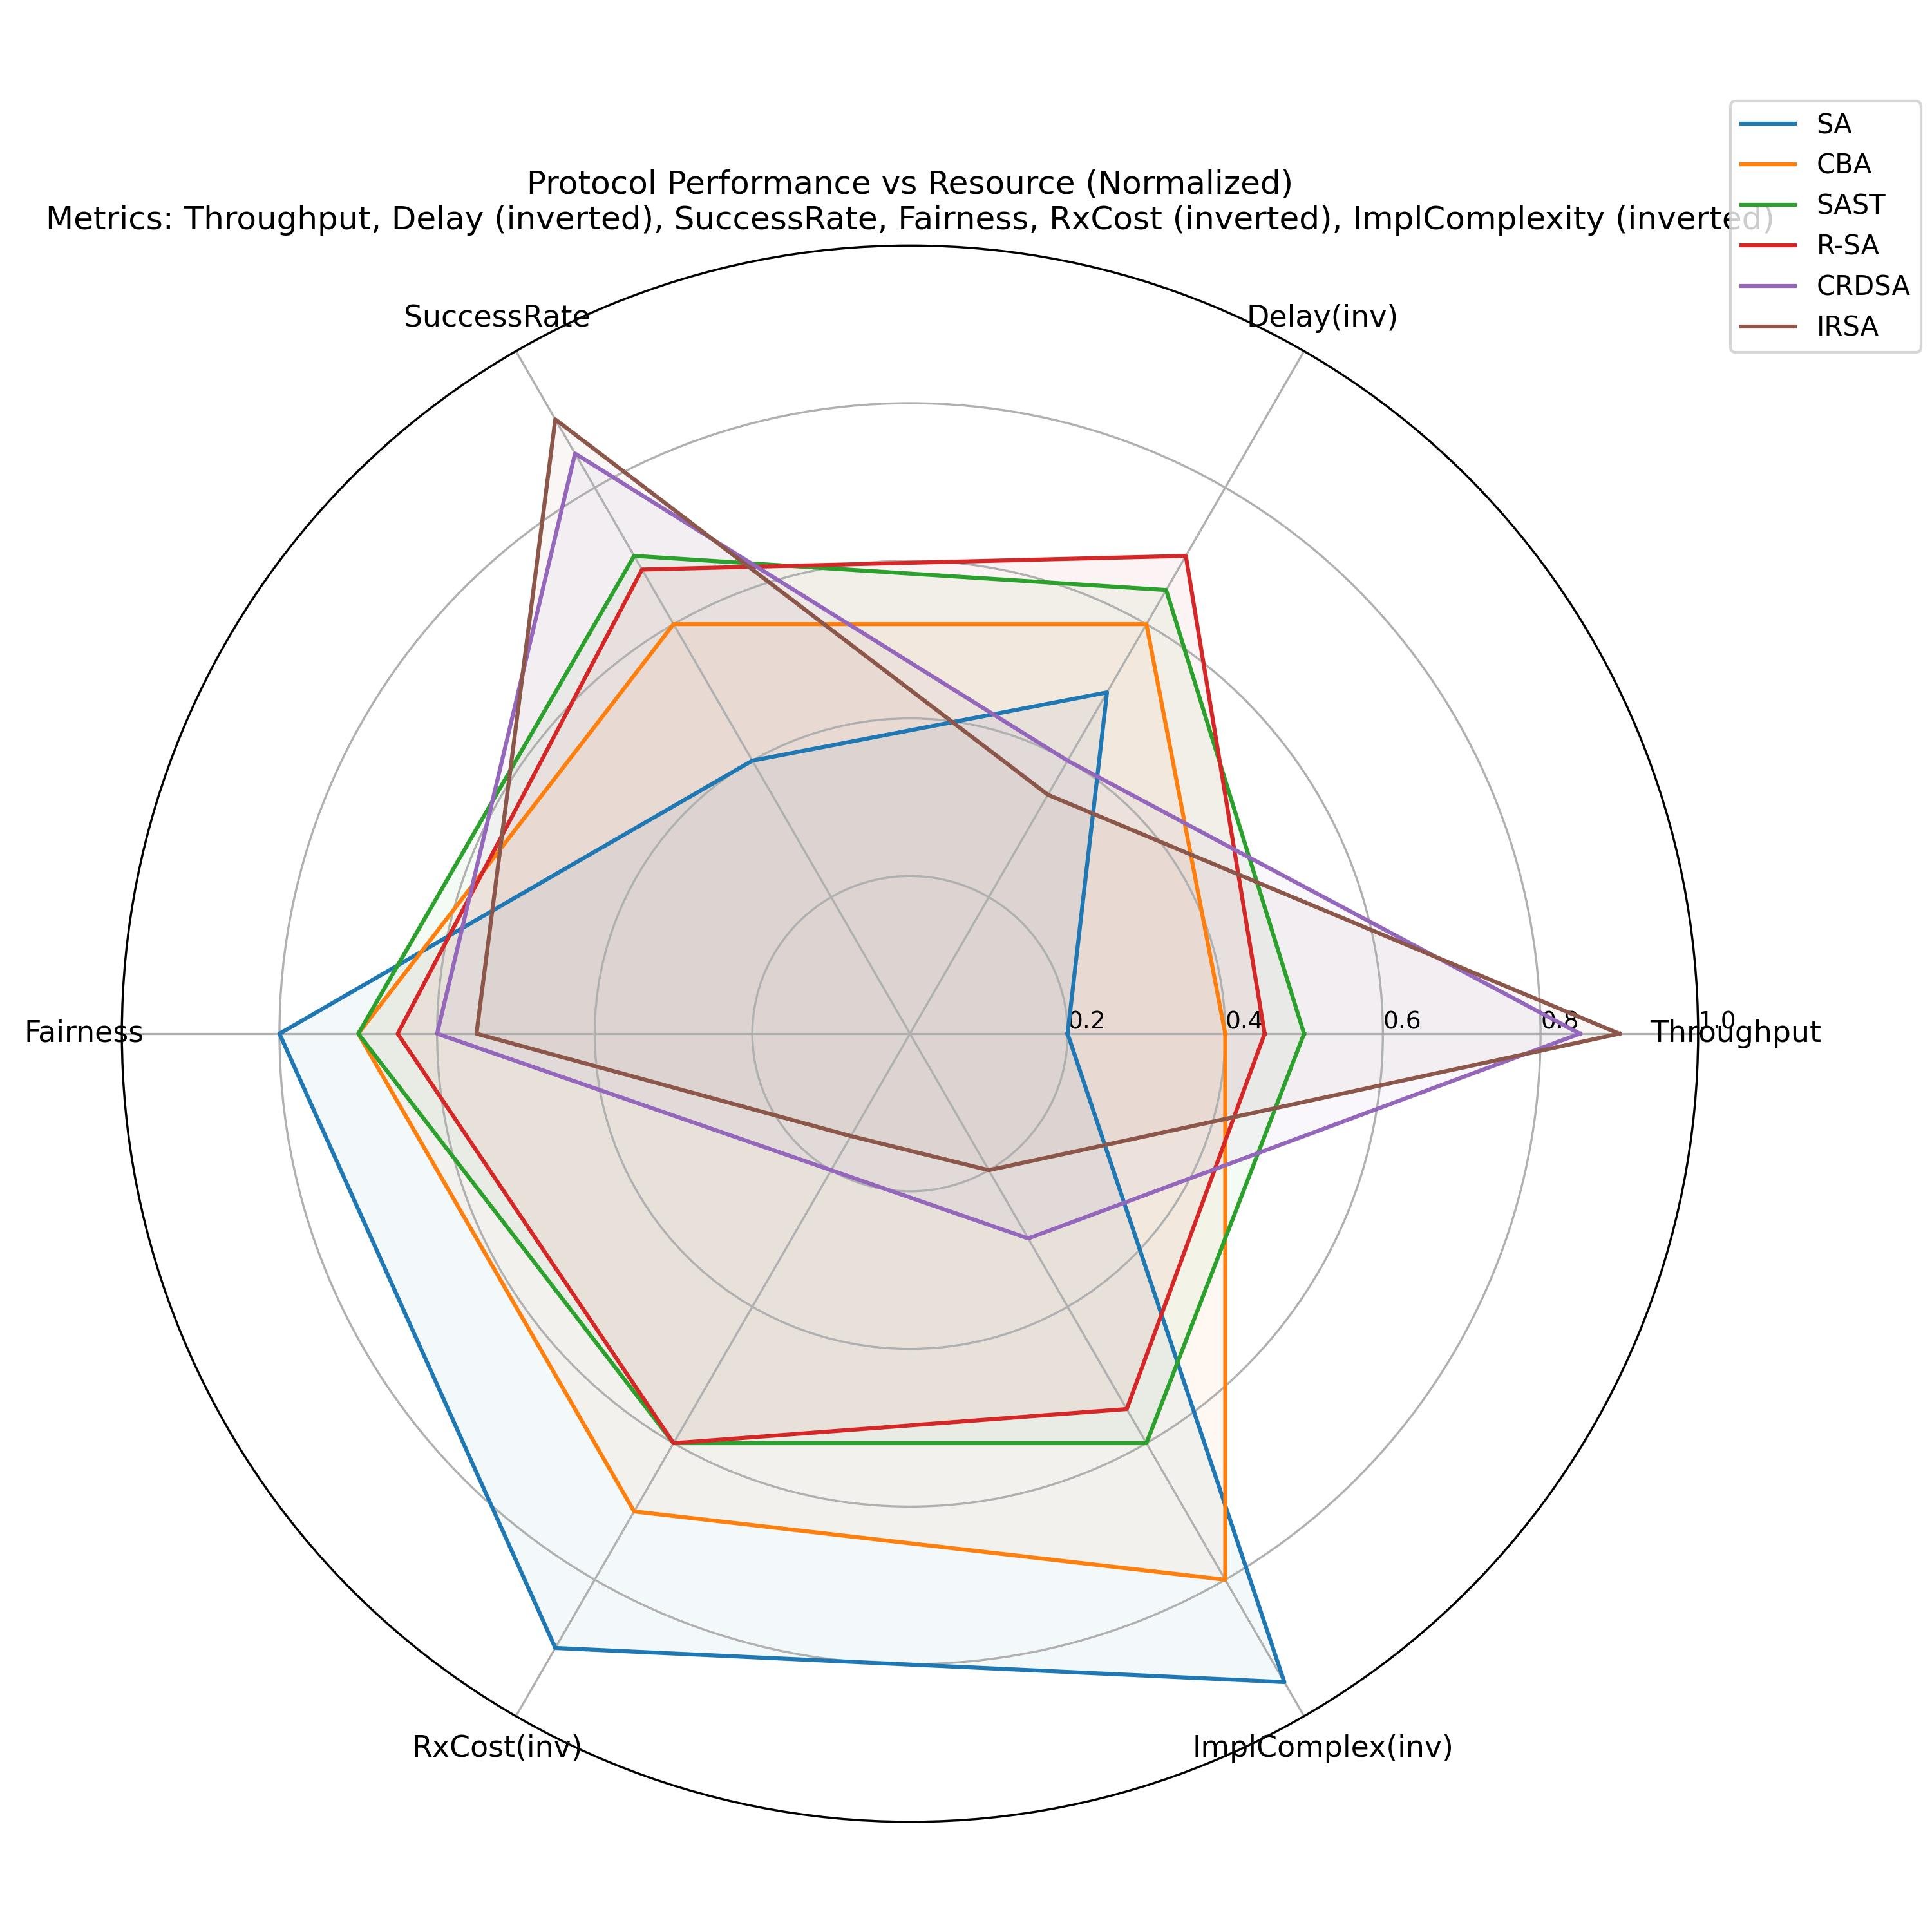
\includegraphics[width=0.3\textwidth]{figure/chap5/Sim12.jpg}
% 		\label{fig:protocol_throughput_comparison2}
% 	}
% 	\hfill
% 	\subfloat[周期场景]{
% 		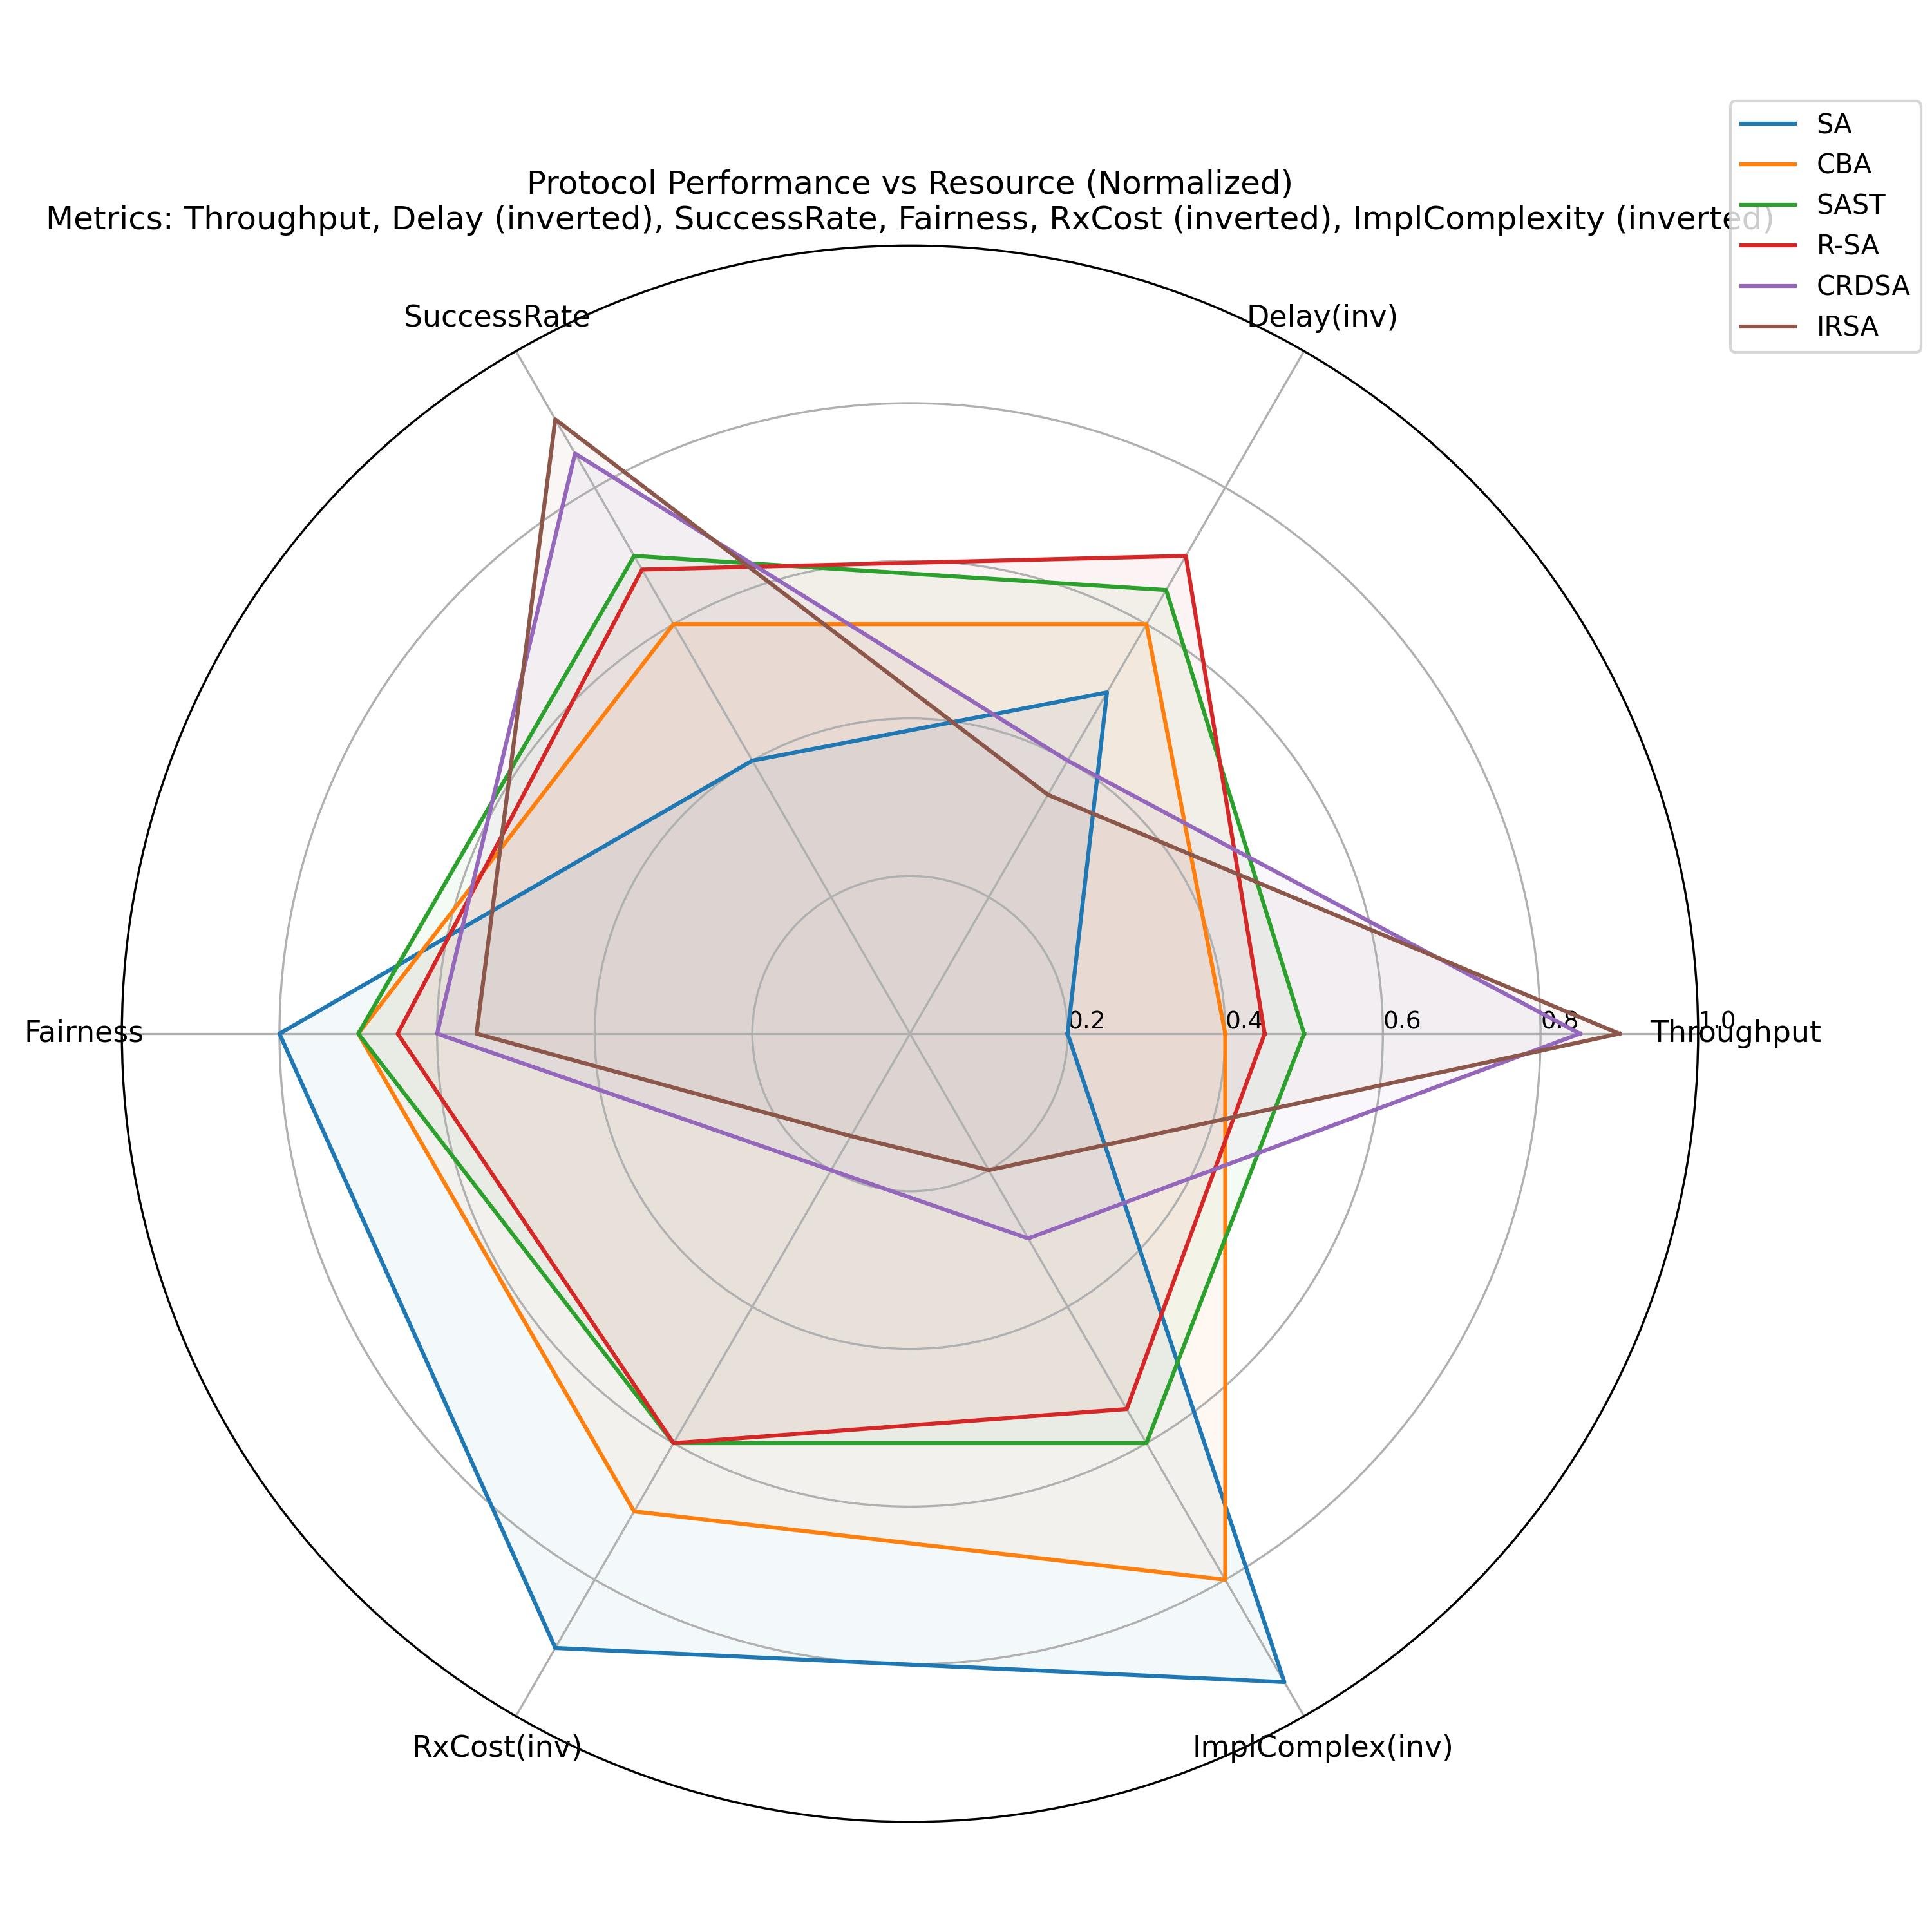
\includegraphics[width=0.3\textwidth]{figure/chap5/Sim13.jpg}
% 		\label{fig:protocol_throughput_comparison3}
% 	}
% 	\caption{不同协议在传输概率变化下的吞吐量对比（固定平均到达率为 $\hat{\lambda}=0.3$）。}
% 	\label{fig:protocol_throughput_comparison}
% \end{figure}

% \textbf{时延对比。} 
% 图~\ref{fig:protocol_delay_comparison} 展示了平均时延 $D$ 随 $\hat{\lambda}$ 的变化趋势。

% \begin{figure}[t]
% 	\centering
% 	\subfloat[均匀场景]{
% 		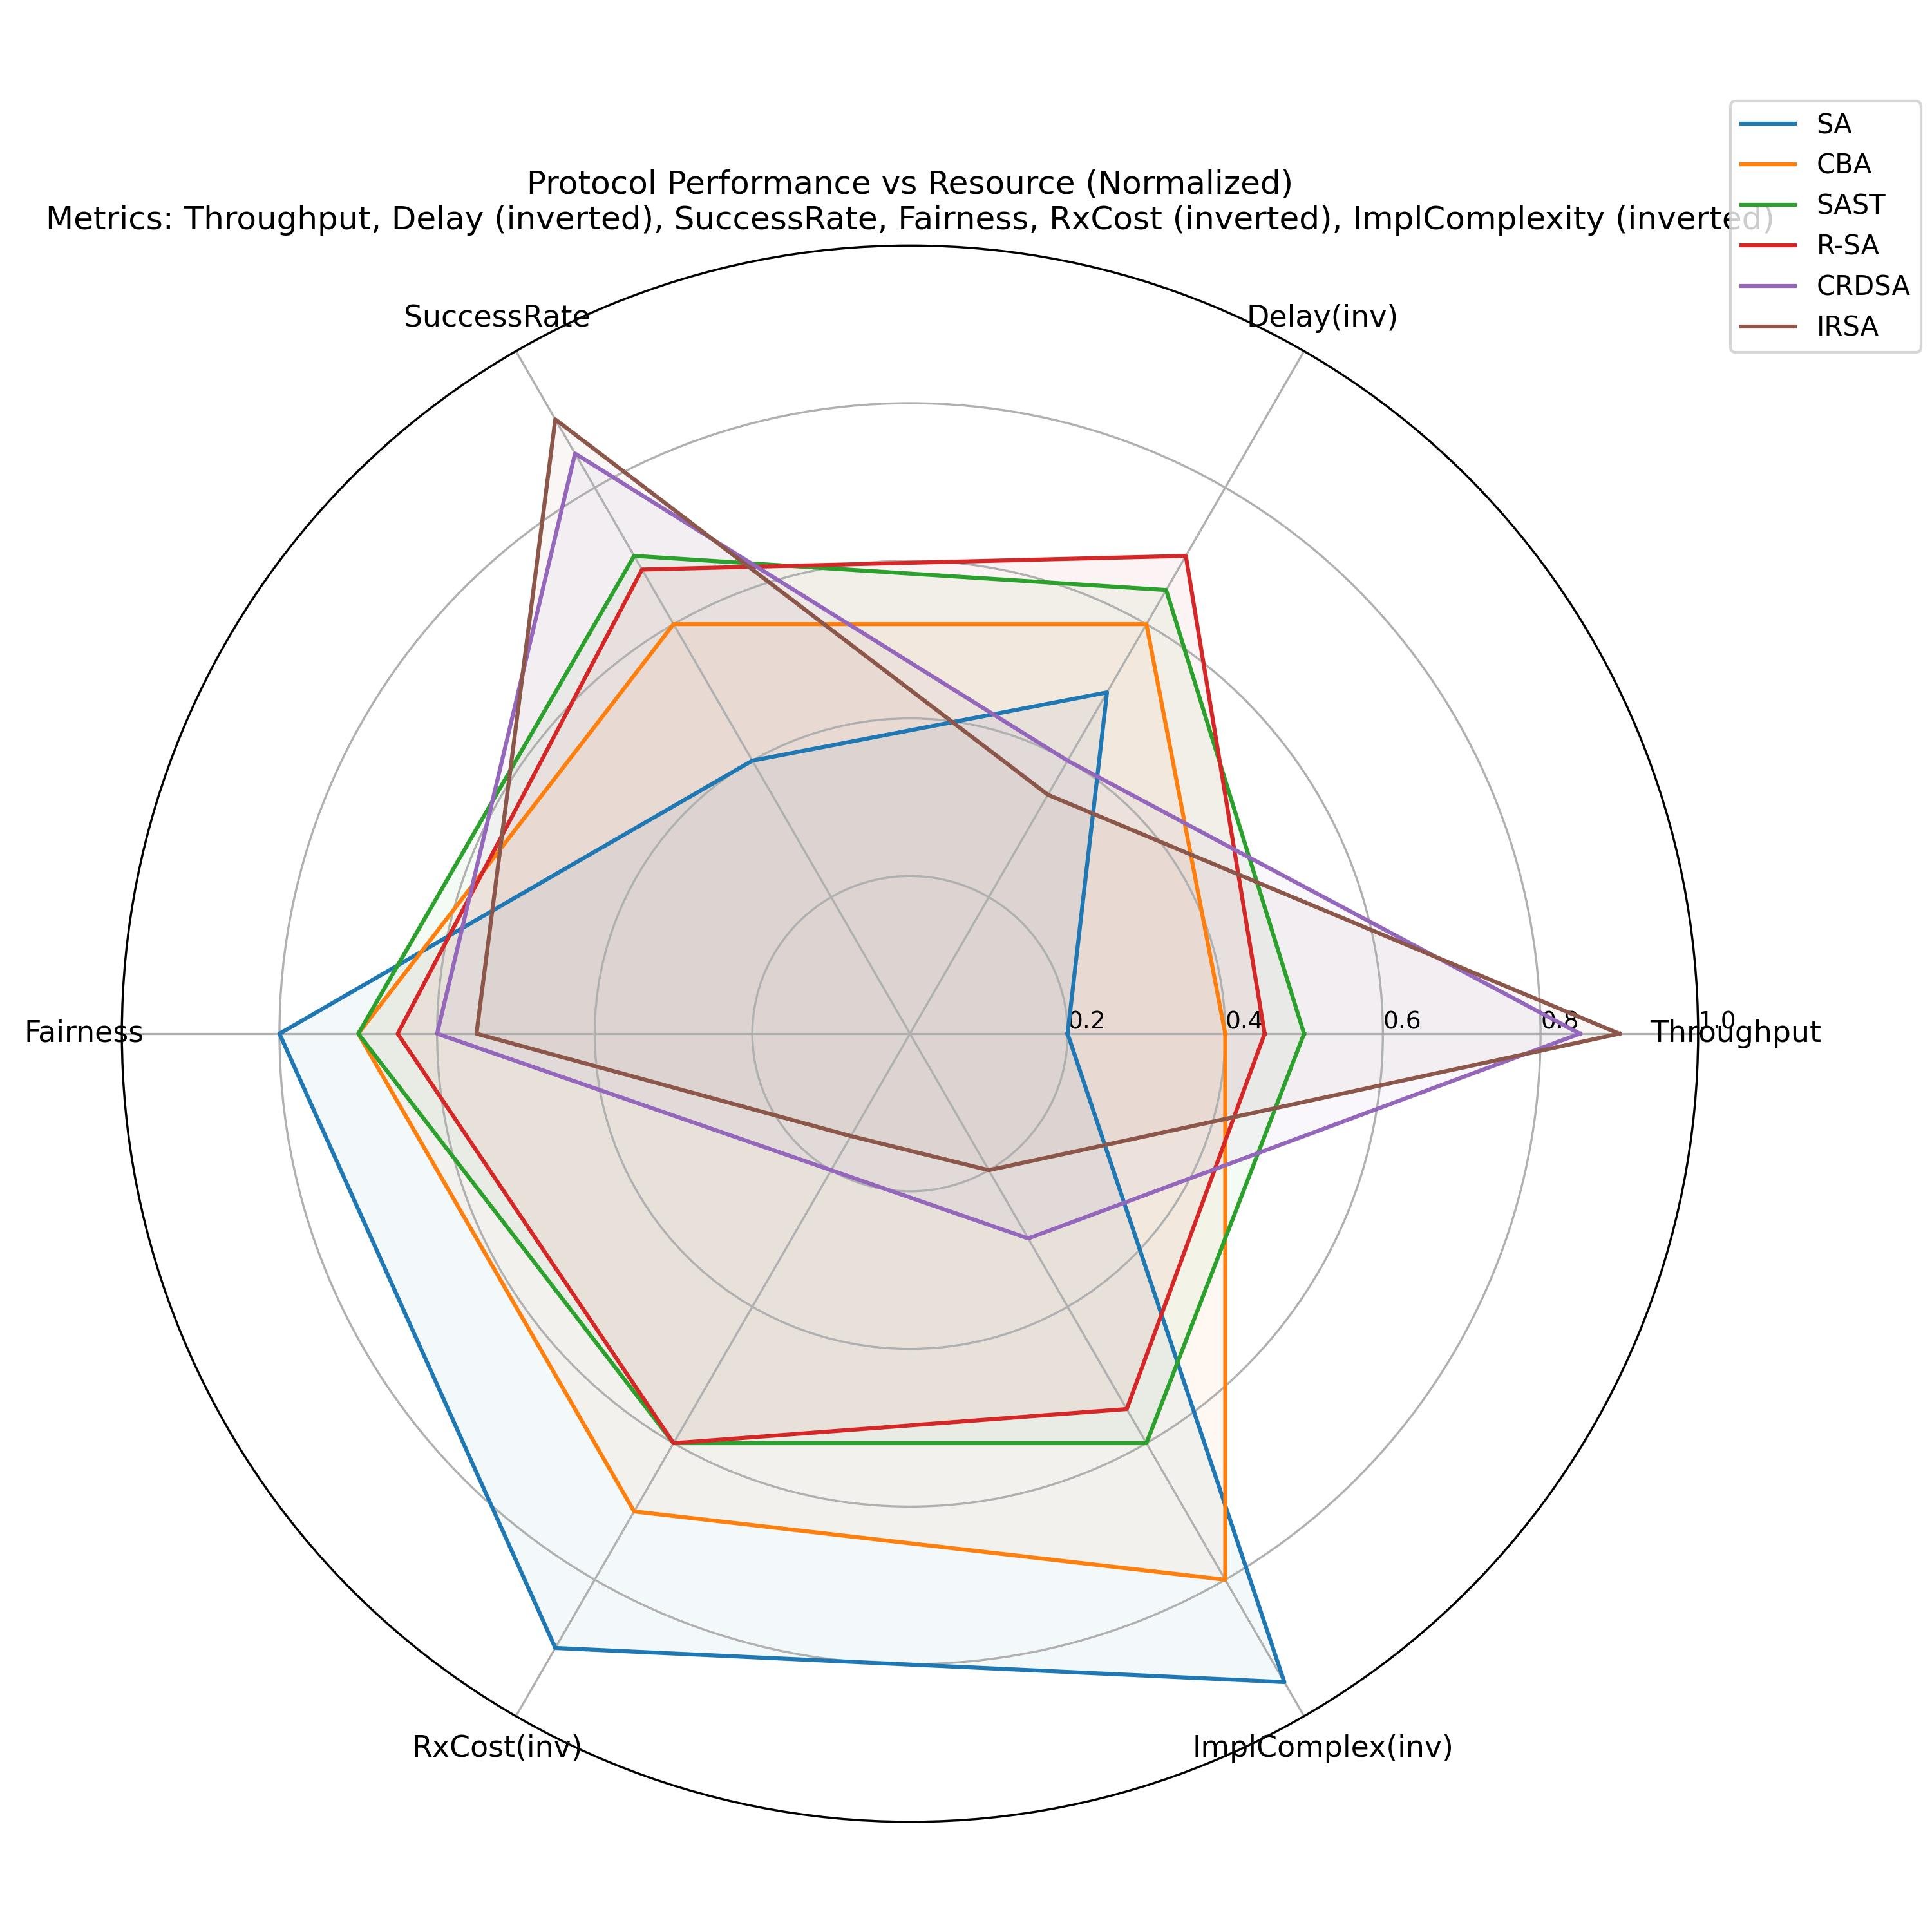
\includegraphics[width=0.3\textwidth]{figure/chap5/Sim21.jpg}
% 		\label{fig:protocol_delay_comparison1}
% 	}
% 	\hfill
% 	\subfloat[突发场景]{
% 		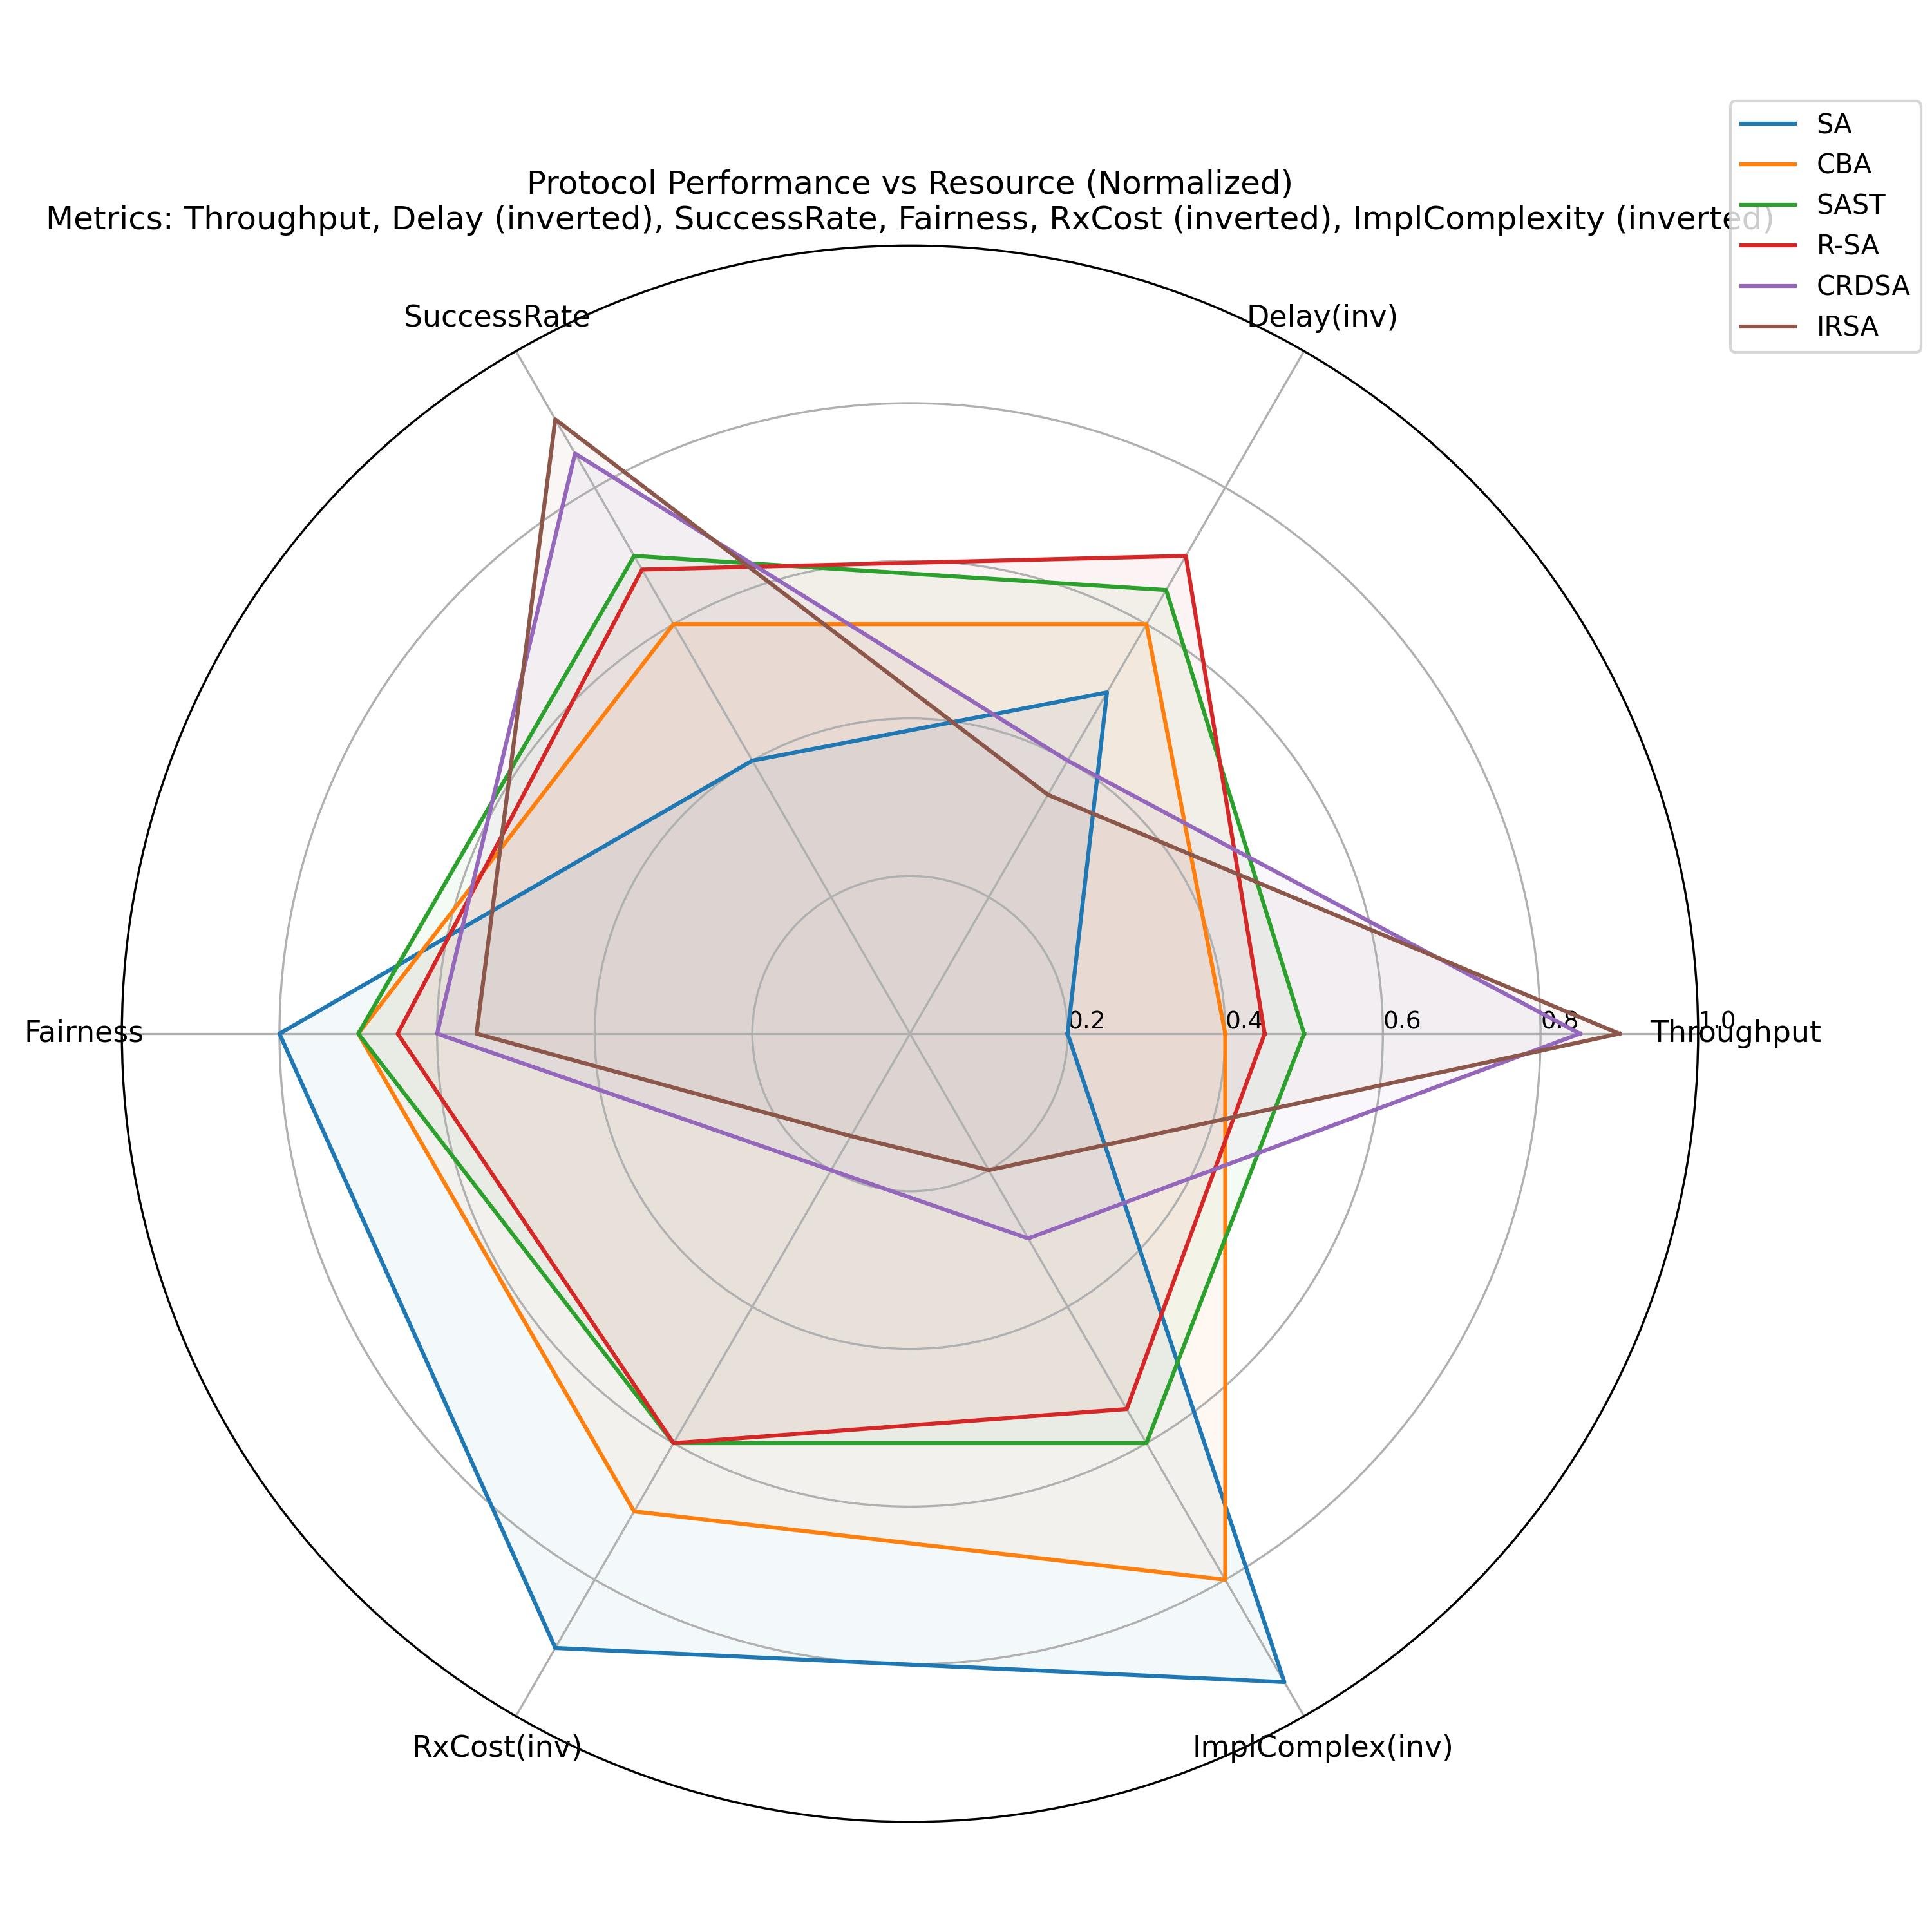
\includegraphics[width=0.3\textwidth]{figure/chap5/Sim22.jpg}
% 		\label{fig:protocol_delay_comparison2}
% 	}
% 	\hfill
% 	\subfloat[周期场景]{
% 		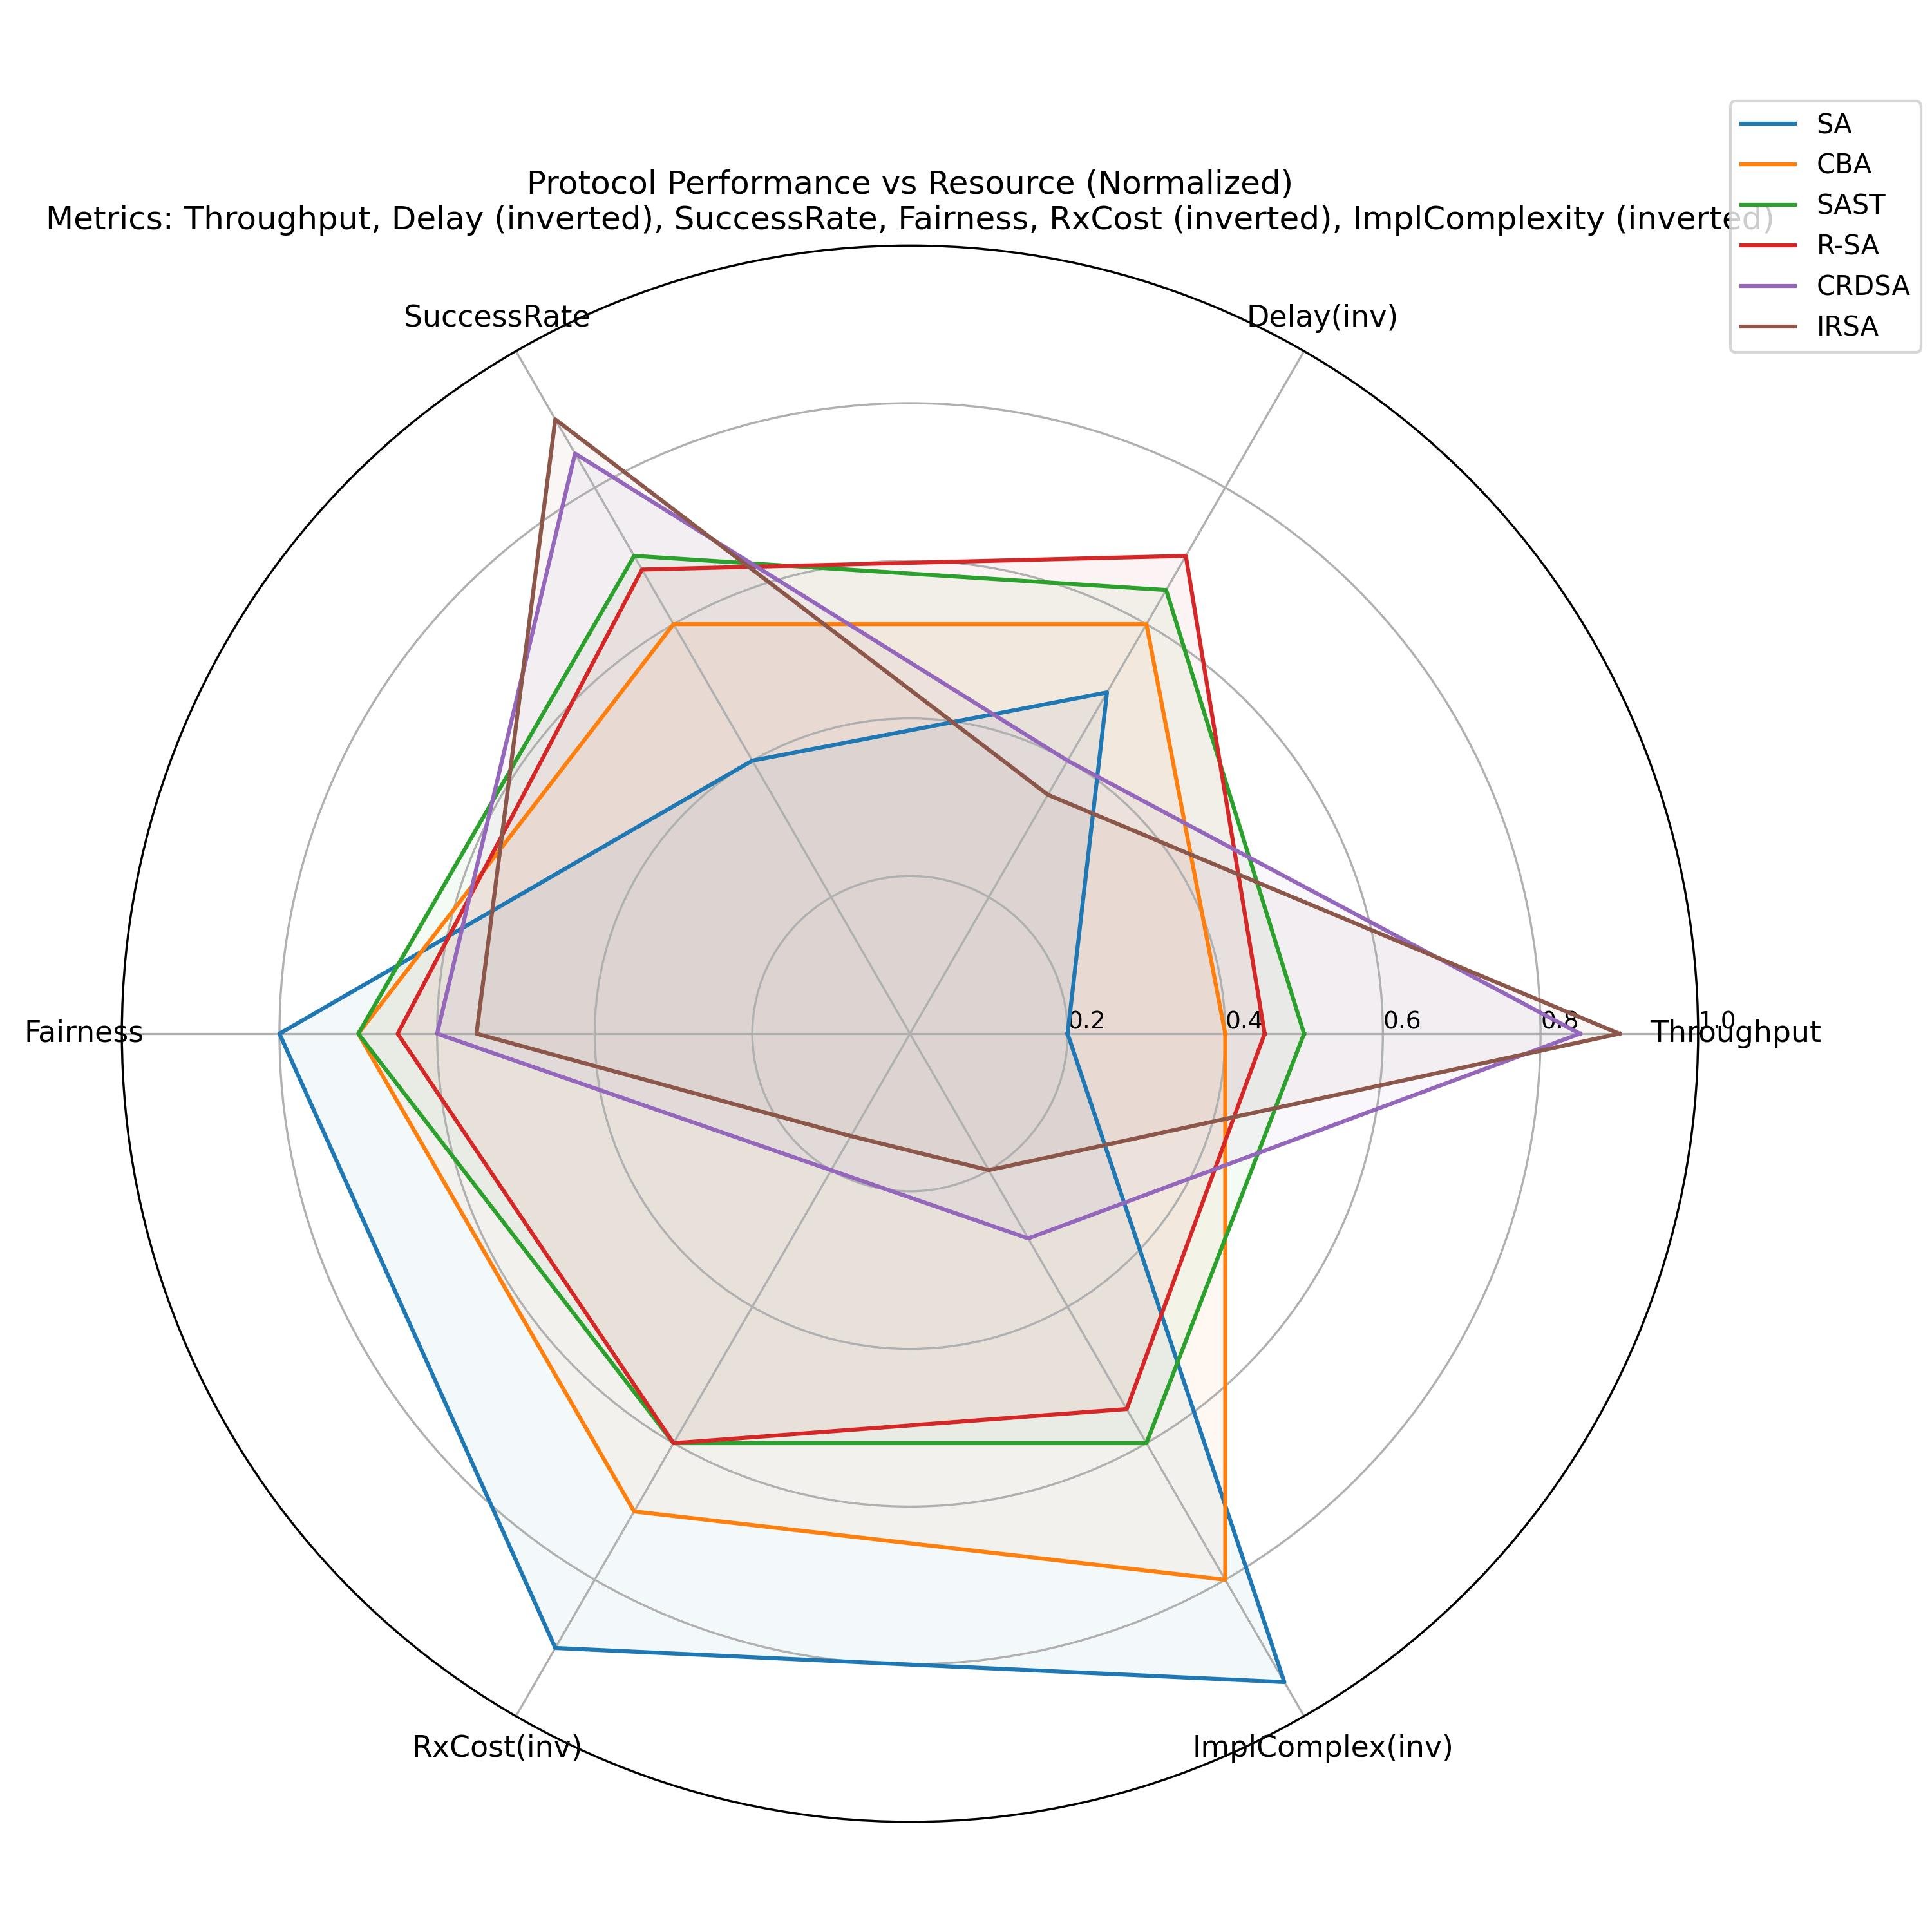
\includegraphics[width=0.3\textwidth]{figure/chap5/Sim23.jpg}
% 		\label{fig:protocol_delay_comparison3}
% 	}
% 	\caption{不同协议在传输概率变化下的平均时延对比（固定平均到达率为 $\hat{\lambda}=0.3$）。}
% 	\label{fig:protocol_delay_comparison}
% \end{figure}


% \textbf{公平性评估。} 
% 图~\ref{fig:protocol_fairness_comparison} 给出了公平性指标（Jain 指数）在不同协议下的变化特征。
% \begin{figure}[t]
% 	\centering
% 	\subfloat[均匀场景]{
% 		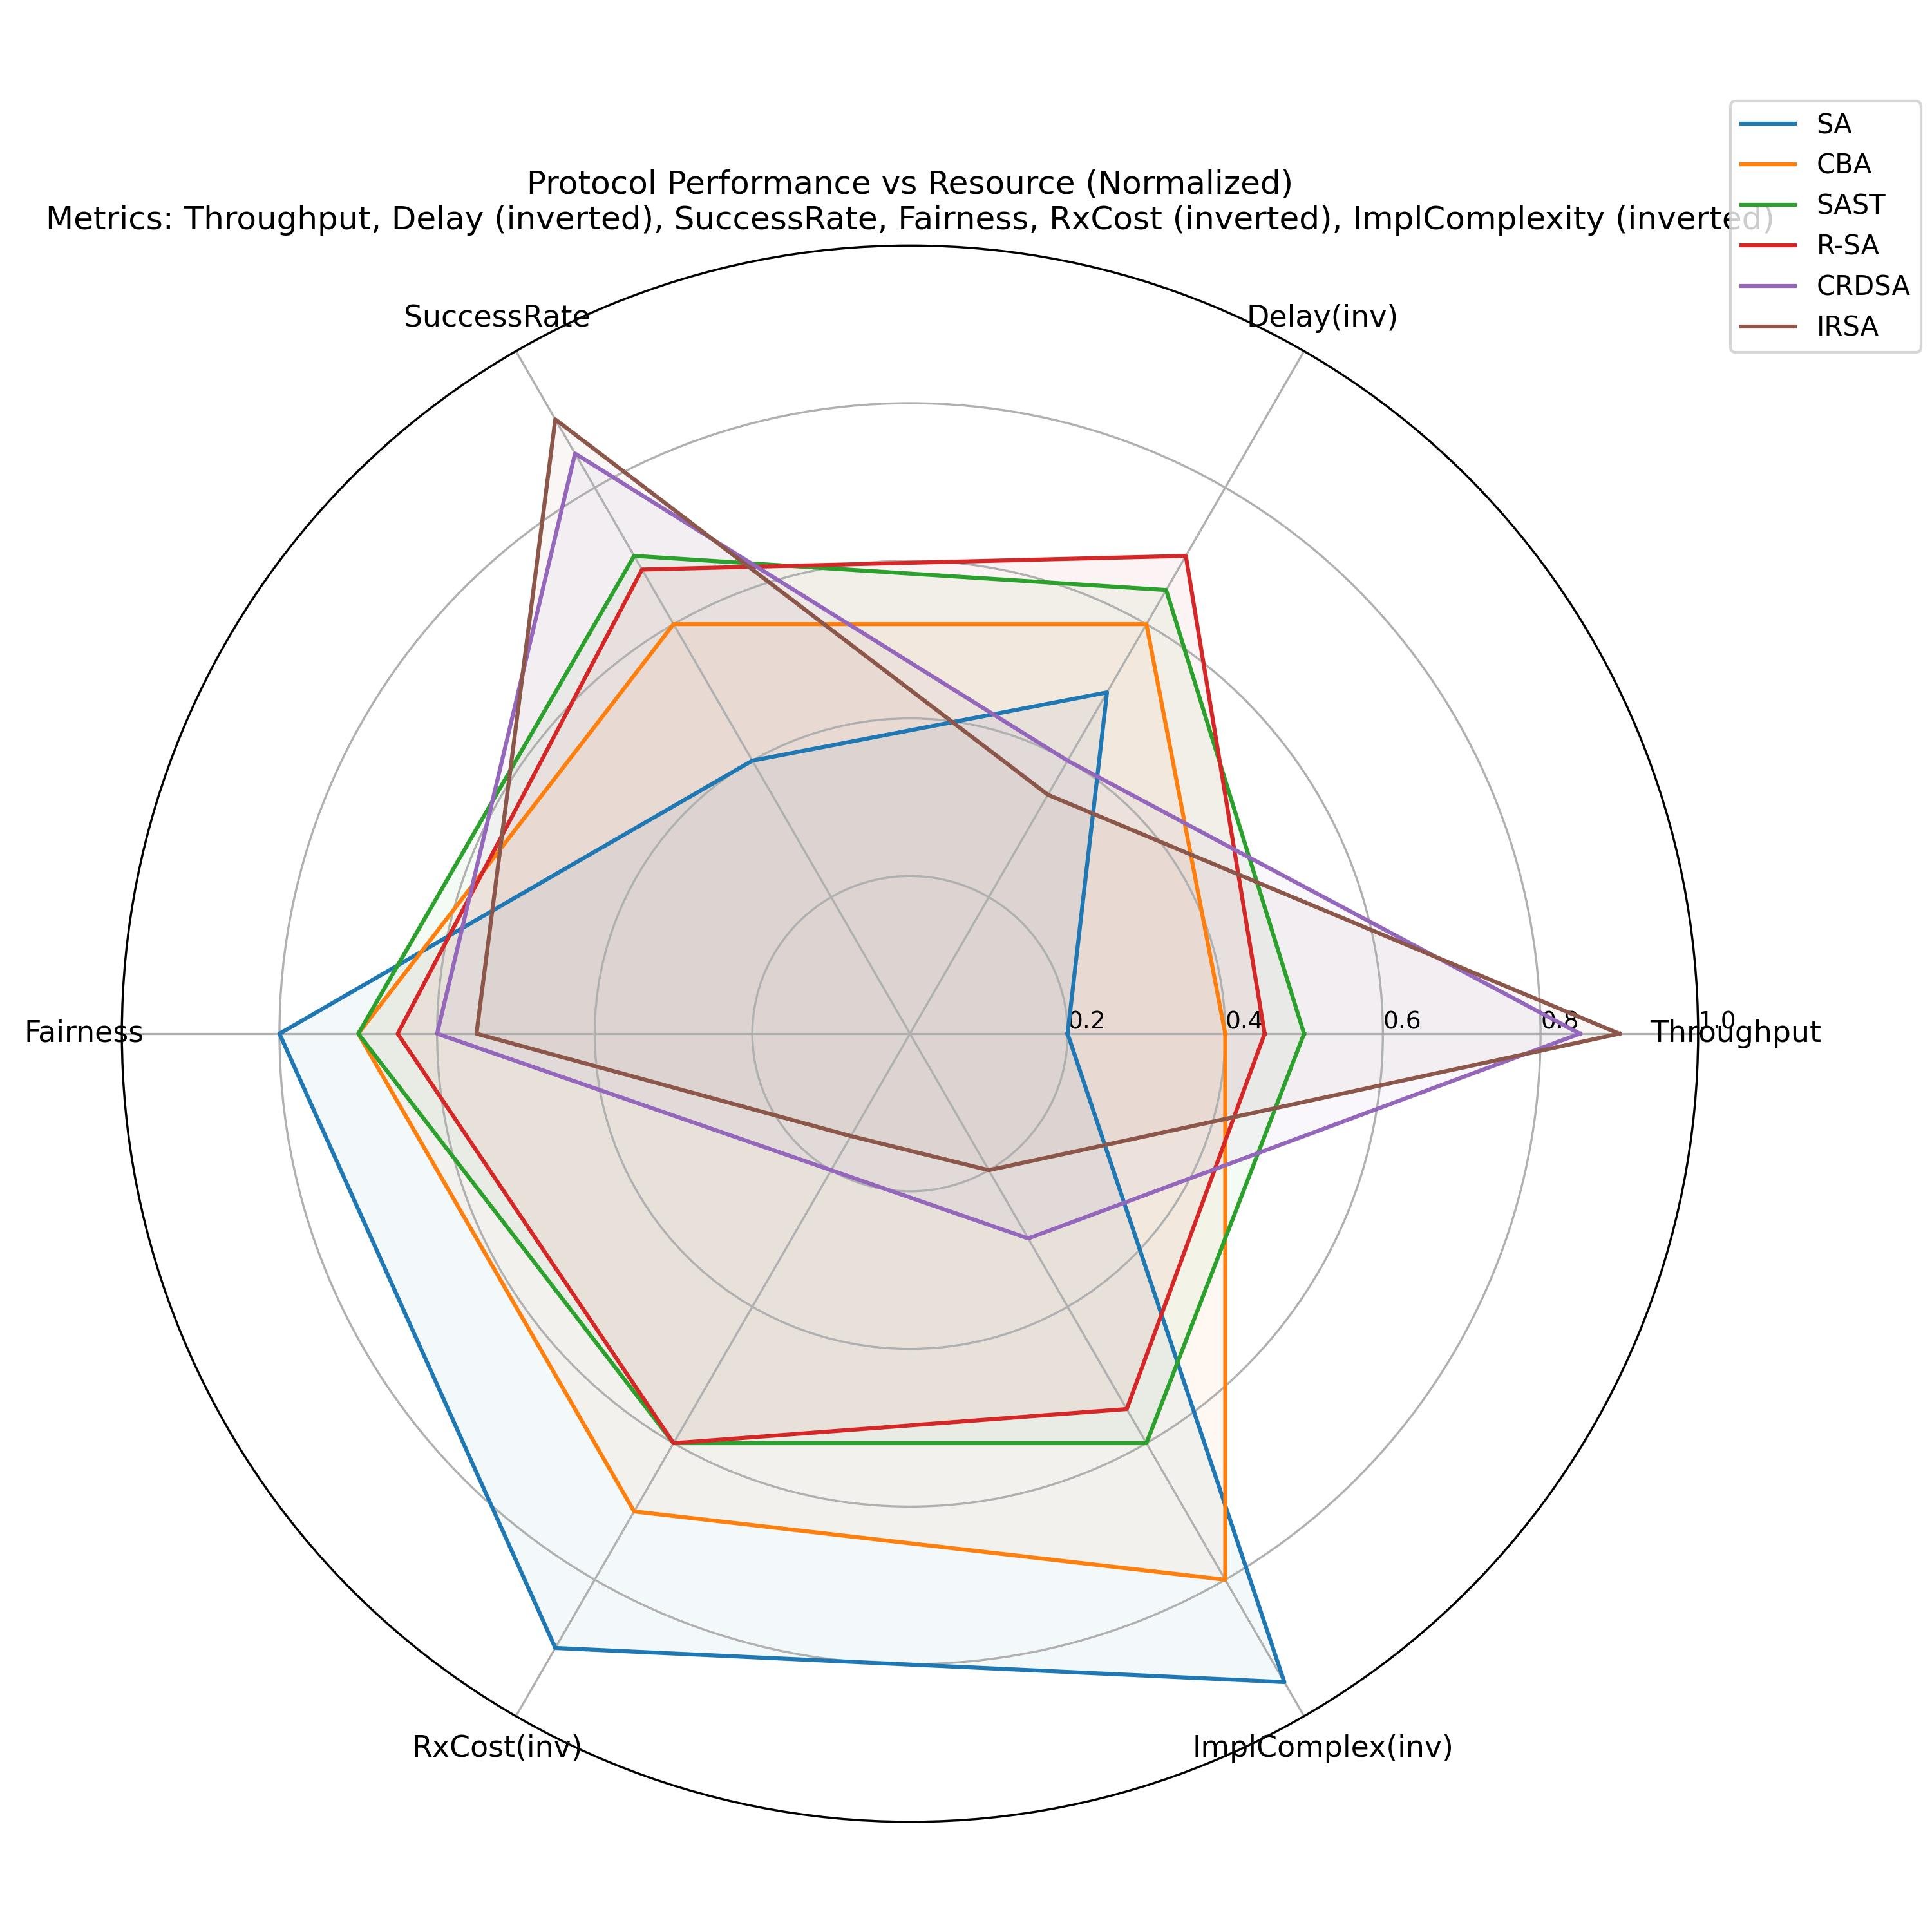
\includegraphics[width=0.3\textwidth]{figure/chap5/Sim31.jpg}
% 		\label{fig:protocol_fairness_comparison1}
% 	}
% 	\hfill
% 	\subfloat[突发场景]{
% 		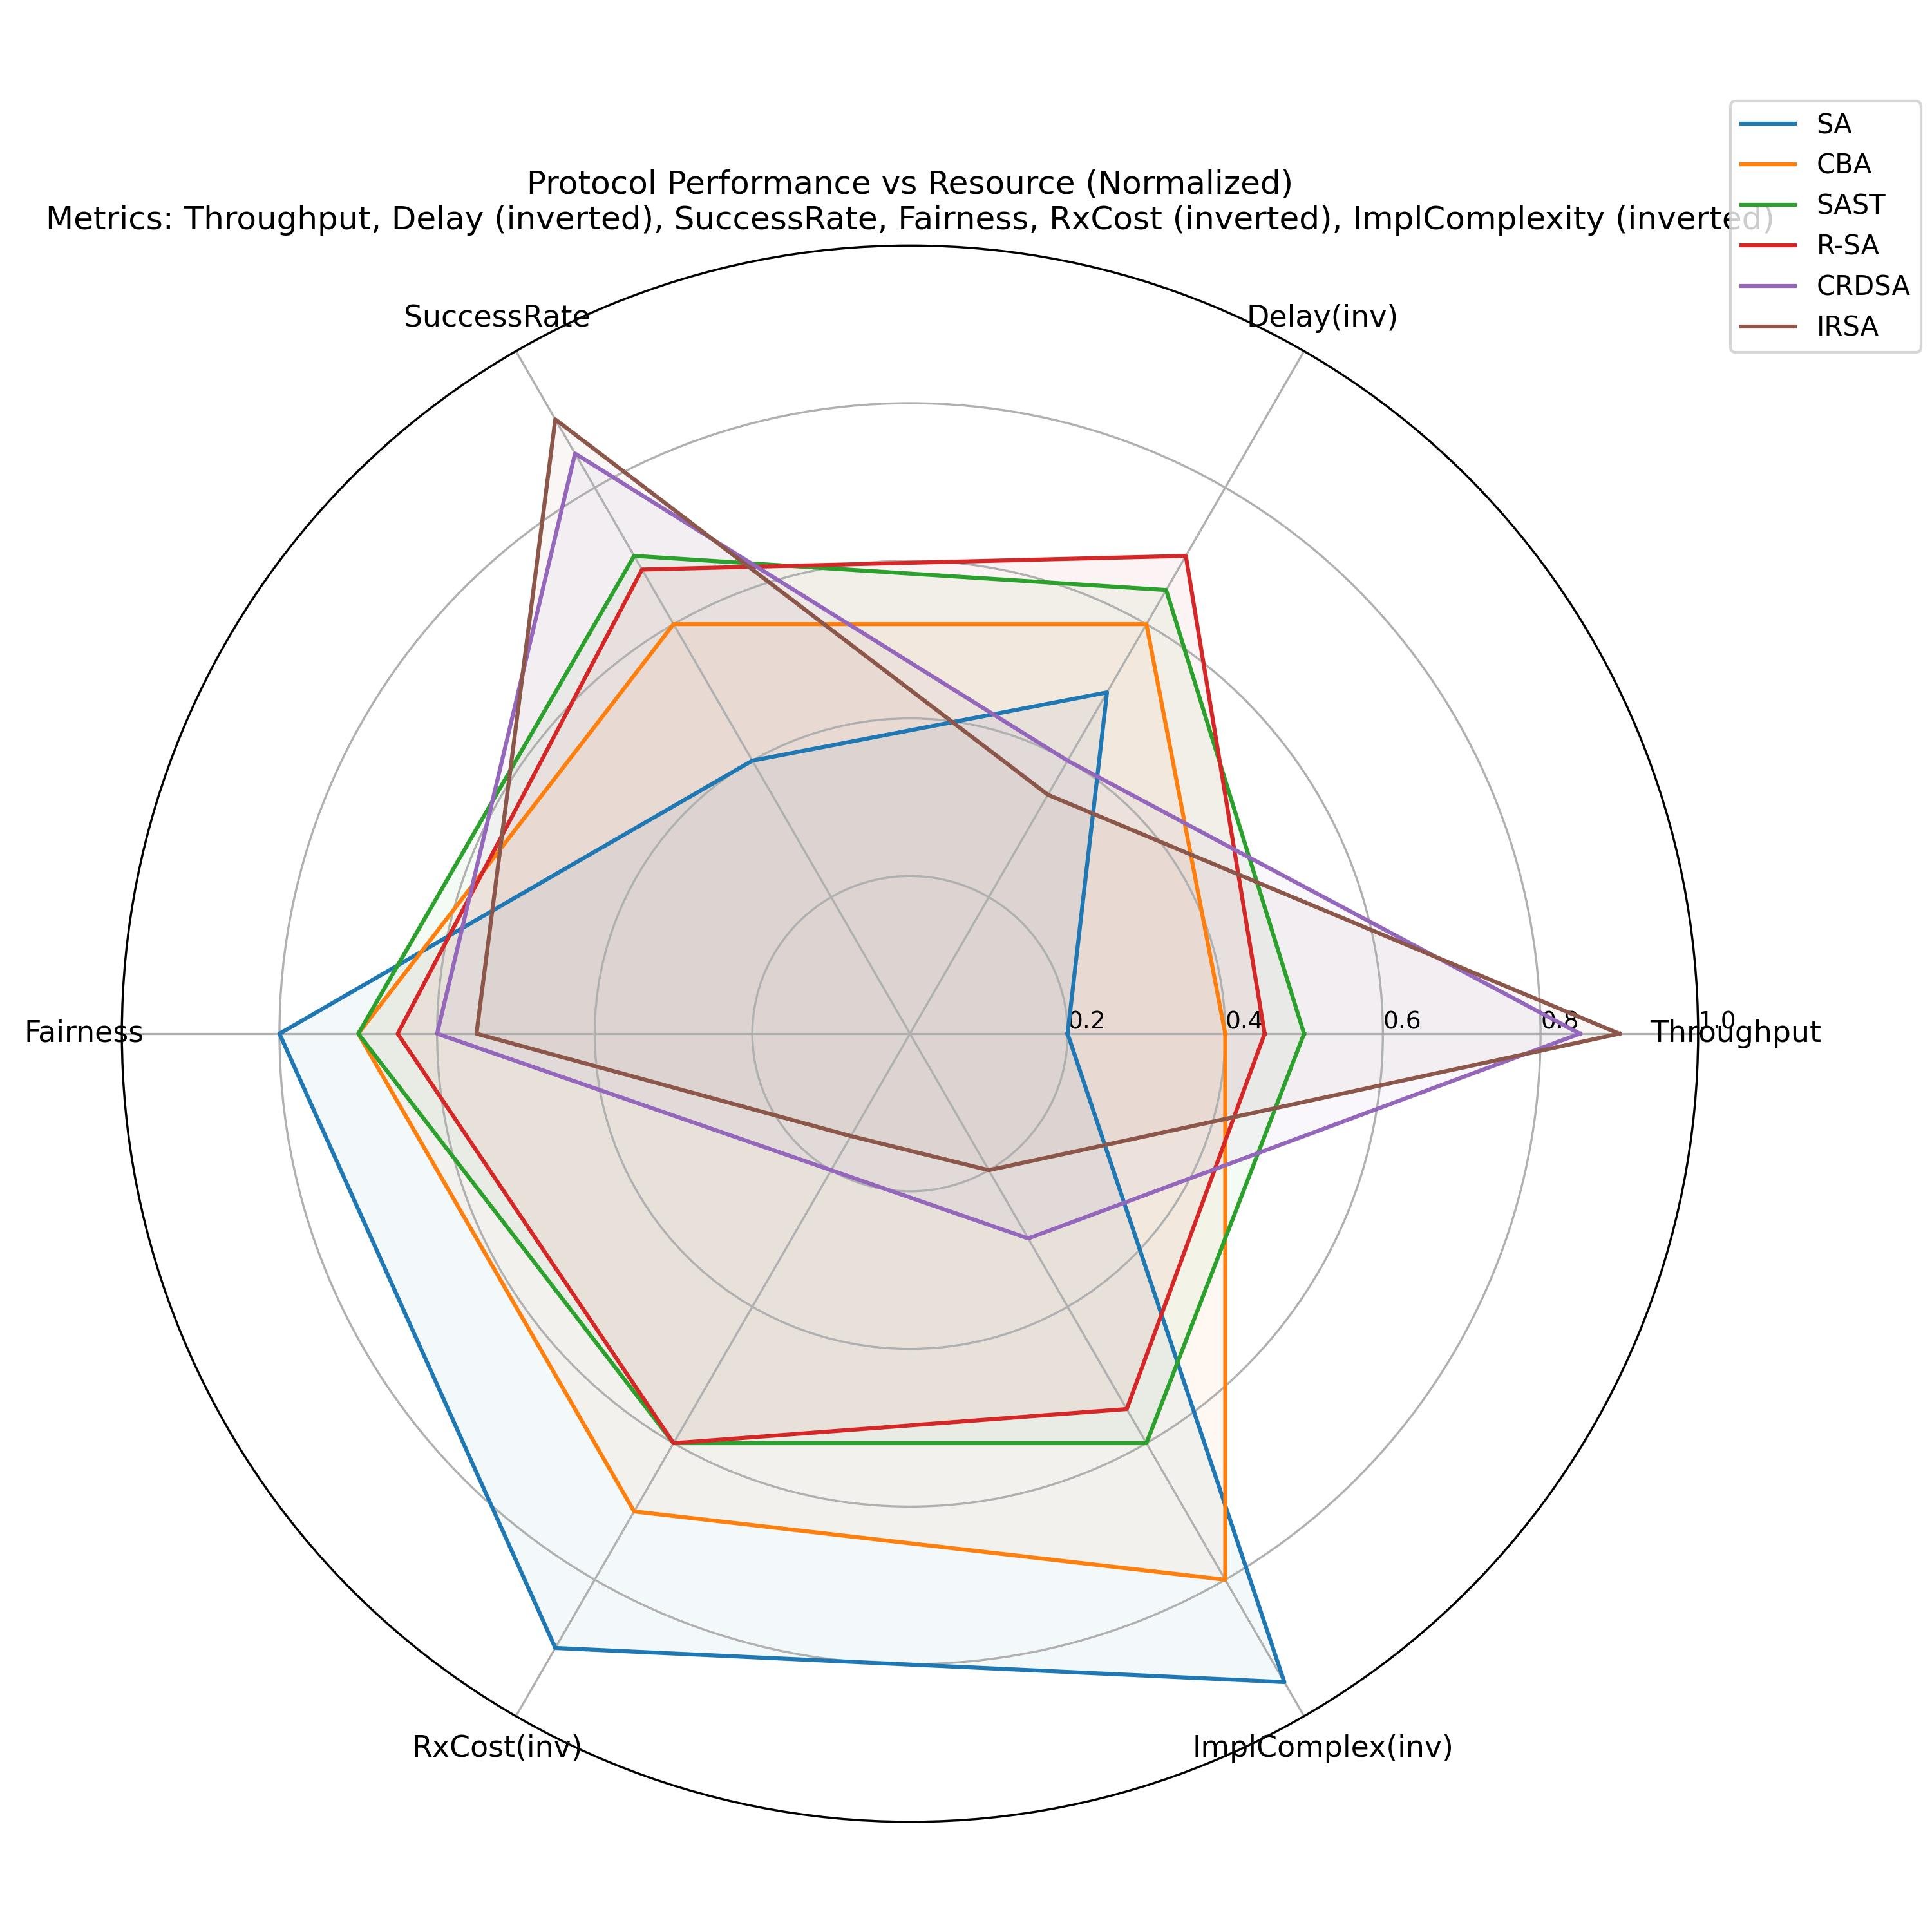
\includegraphics[width=0.3\textwidth]{figure/chap5/Sim32.jpg}
% 		\label{fig:protocol_fairness_comparison2}
% 	}
% 	\hfill
% 	\subfloat[周期场景]{
% 		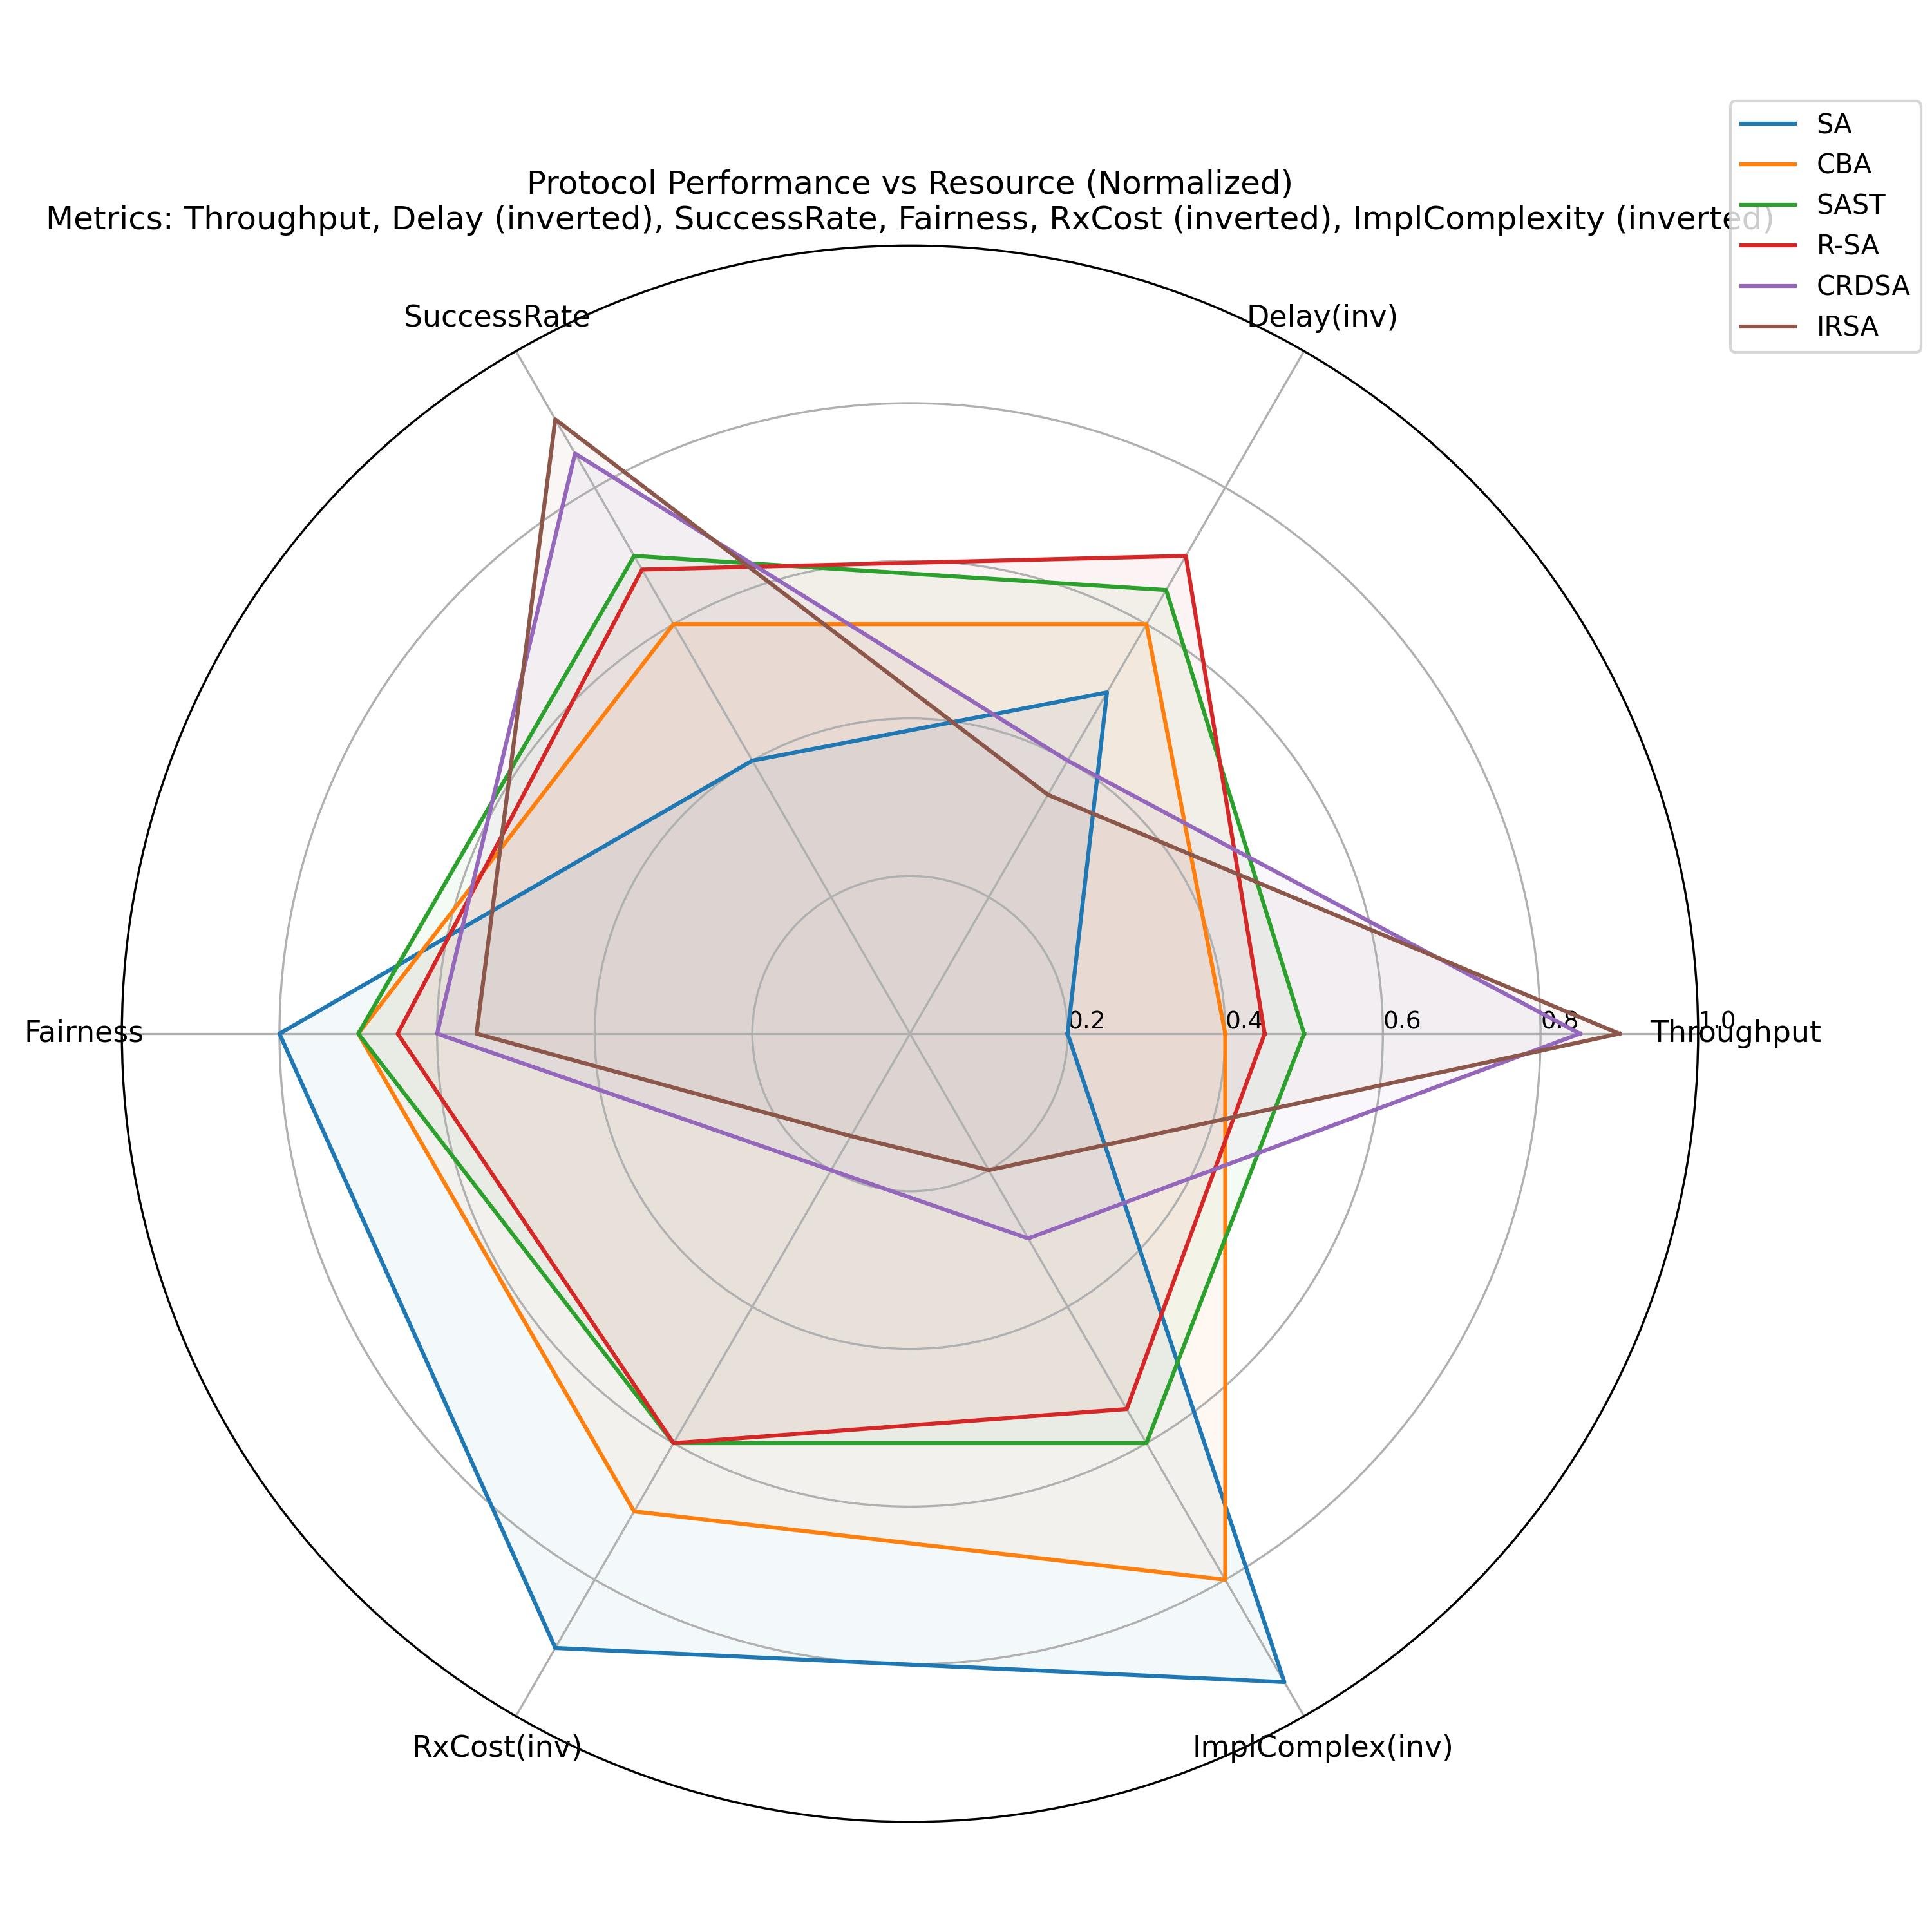
\includegraphics[width=0.3\textwidth]{figure/chap5/Sim33.jpg}
% 		\label{fig:protocol_fairness_comparison3}
% 	}
% 	\caption{不同协议在传输概率变化下的公平性对比（固定平均到达率为 $\hat{\lambda}=0.3$）。}
% 	\label{fig:protocol_fairness_comparison}
% \end{figure}


% \textbf{综合效用评估。} 
% 本小节采用综合效用 $U(\tilde{\mathbf{y}})$ 的效用权重设置为 $w_{\lambda}=0.4$、$w_D=0.3$、$w_J=0.2$、$w_S=0.1$。图~\ref{fig:protocol_utility_comparison} 展示了基于式~\eqref{eq:chap5_constrained} 定义的综合效用 $U(\tilde{\mathbf{y}})$ 对比结果。

% \begin{figure}[t]
% 	\centering
% 	\subfloat[均匀场景]{
% 		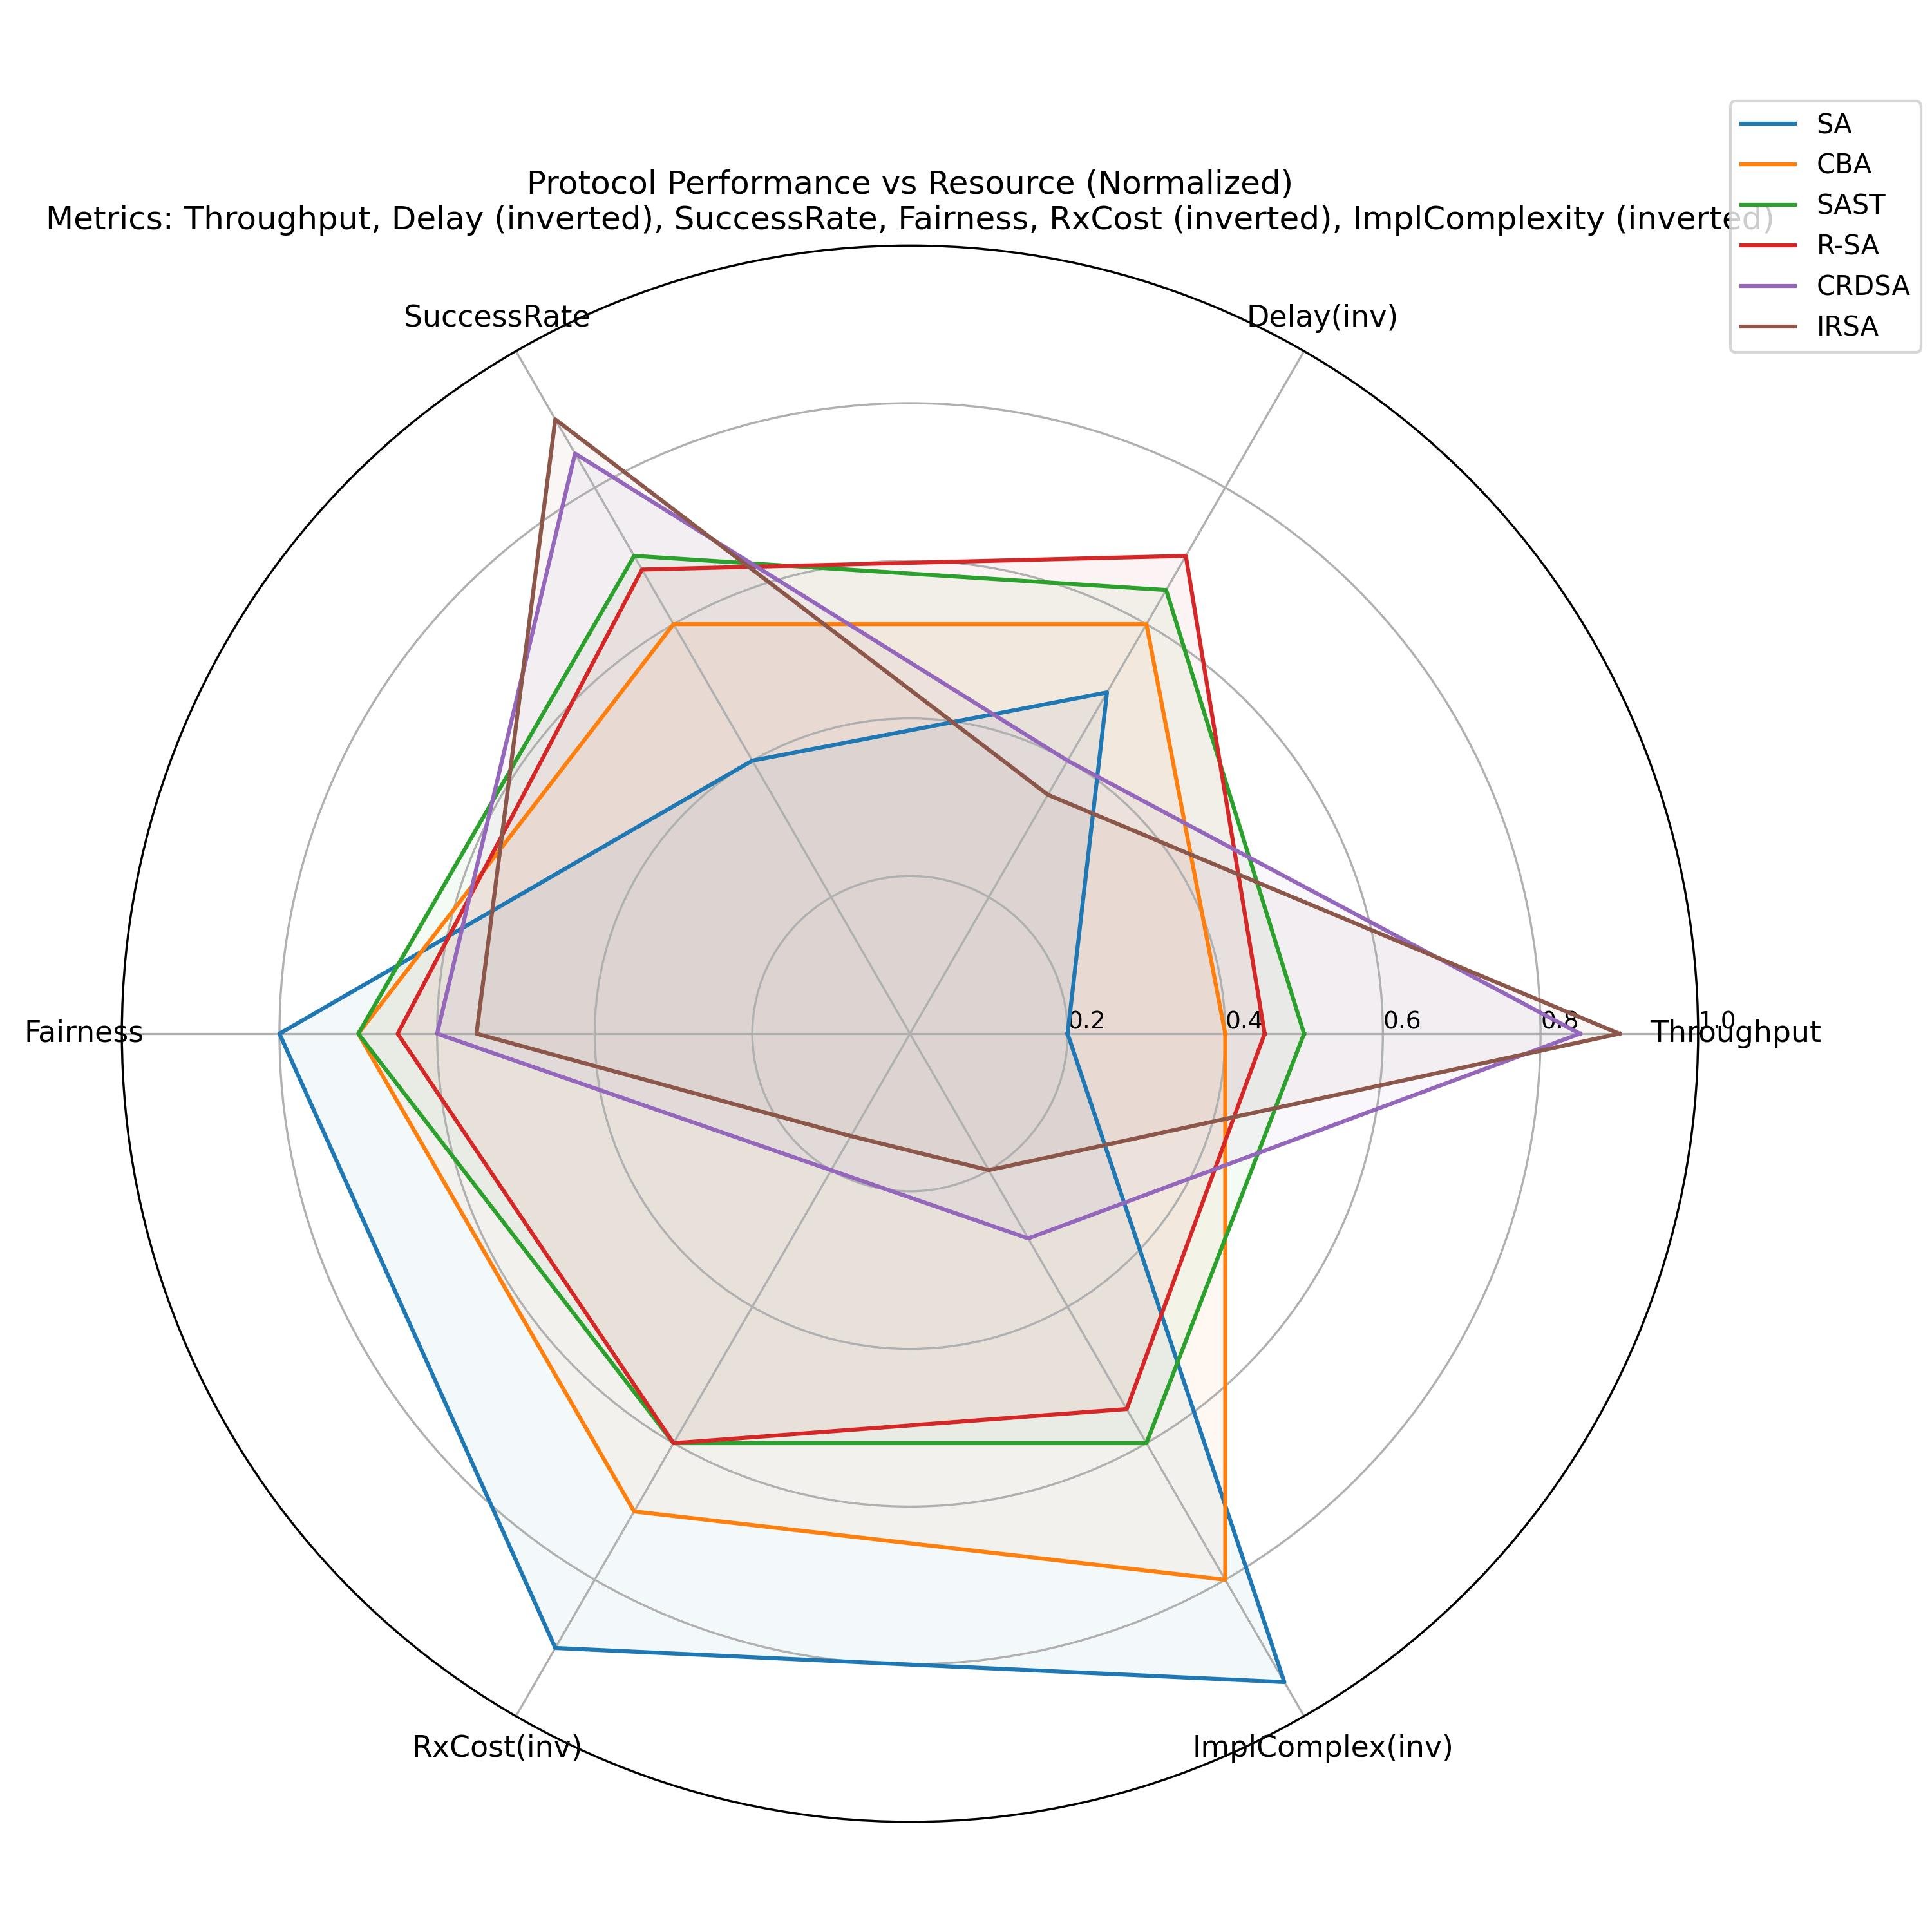
\includegraphics[width=0.3\textwidth]{figure/chap5/Sim41.jpg}
% 		\label{fig:protocol_utility_comparison1}
% 	}
% 	\hfill
% 	\subfloat[突发场景]{
% 		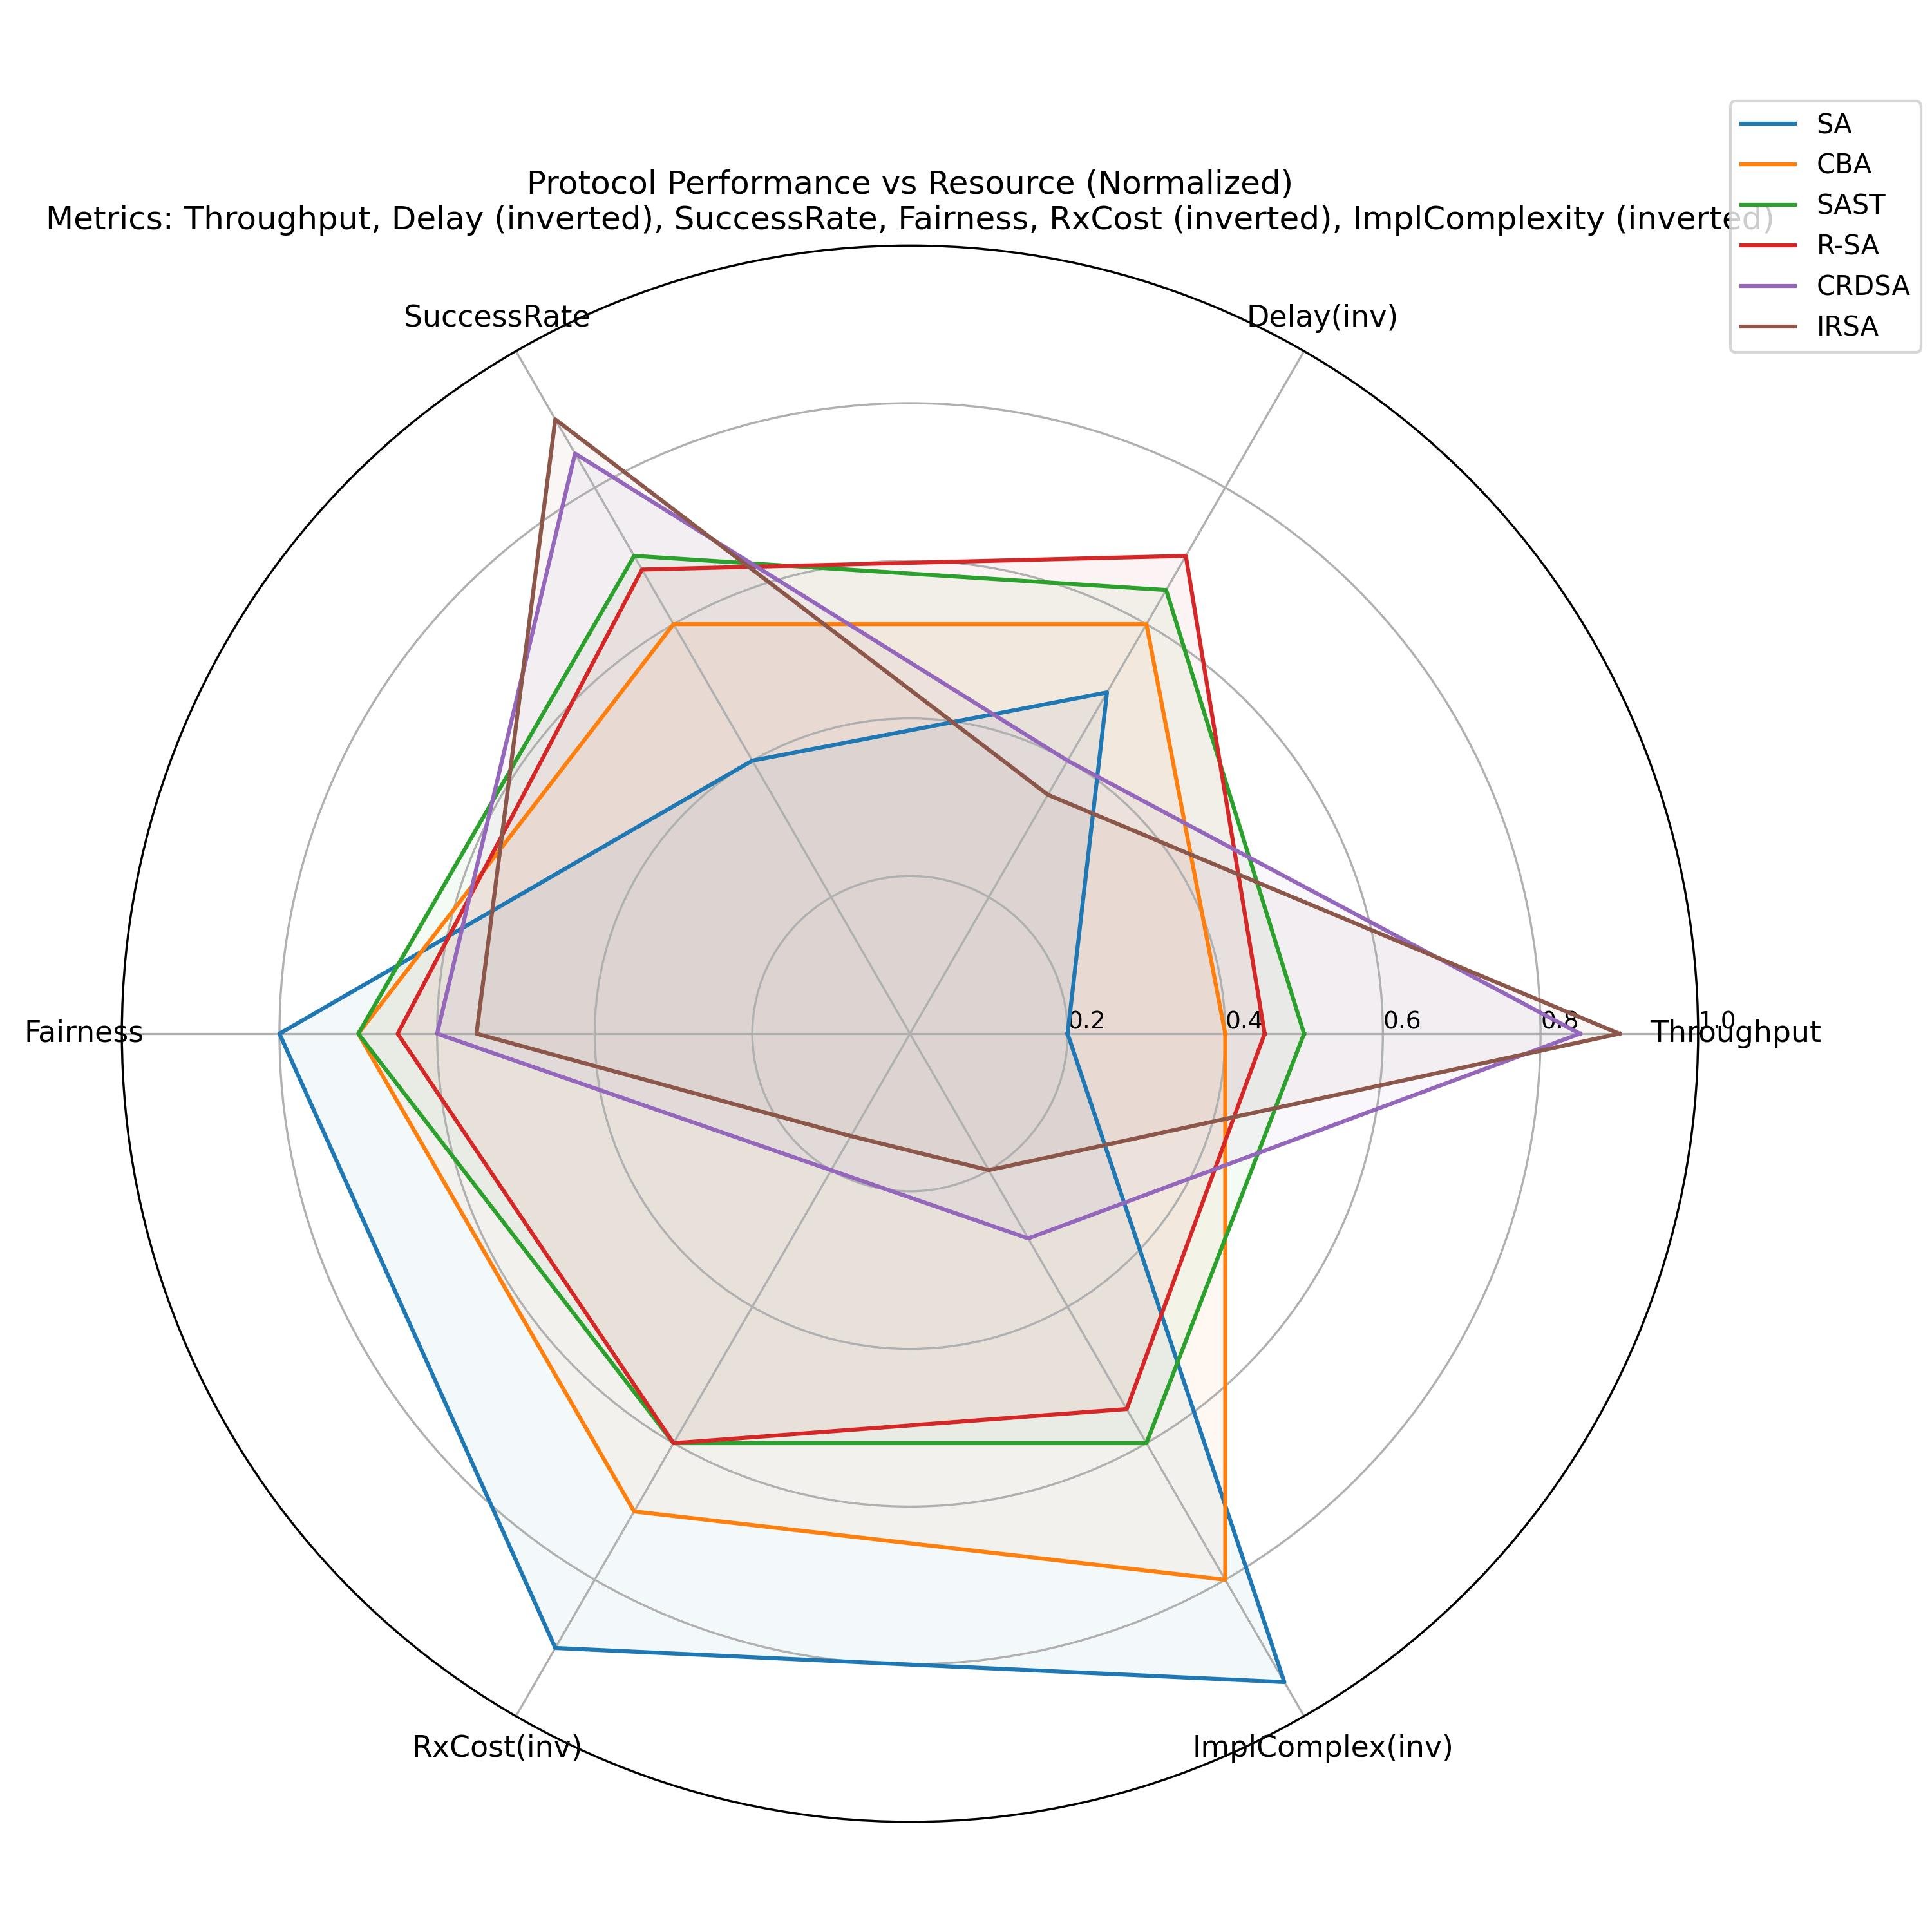
\includegraphics[width=0.3\textwidth]{figure/chap5/Sim42.jpg}
% 		\label{fig:protocol_utility_comparison2}
% 	}
% 	\hfill
% 	\subfloat[周期场景]{
% 		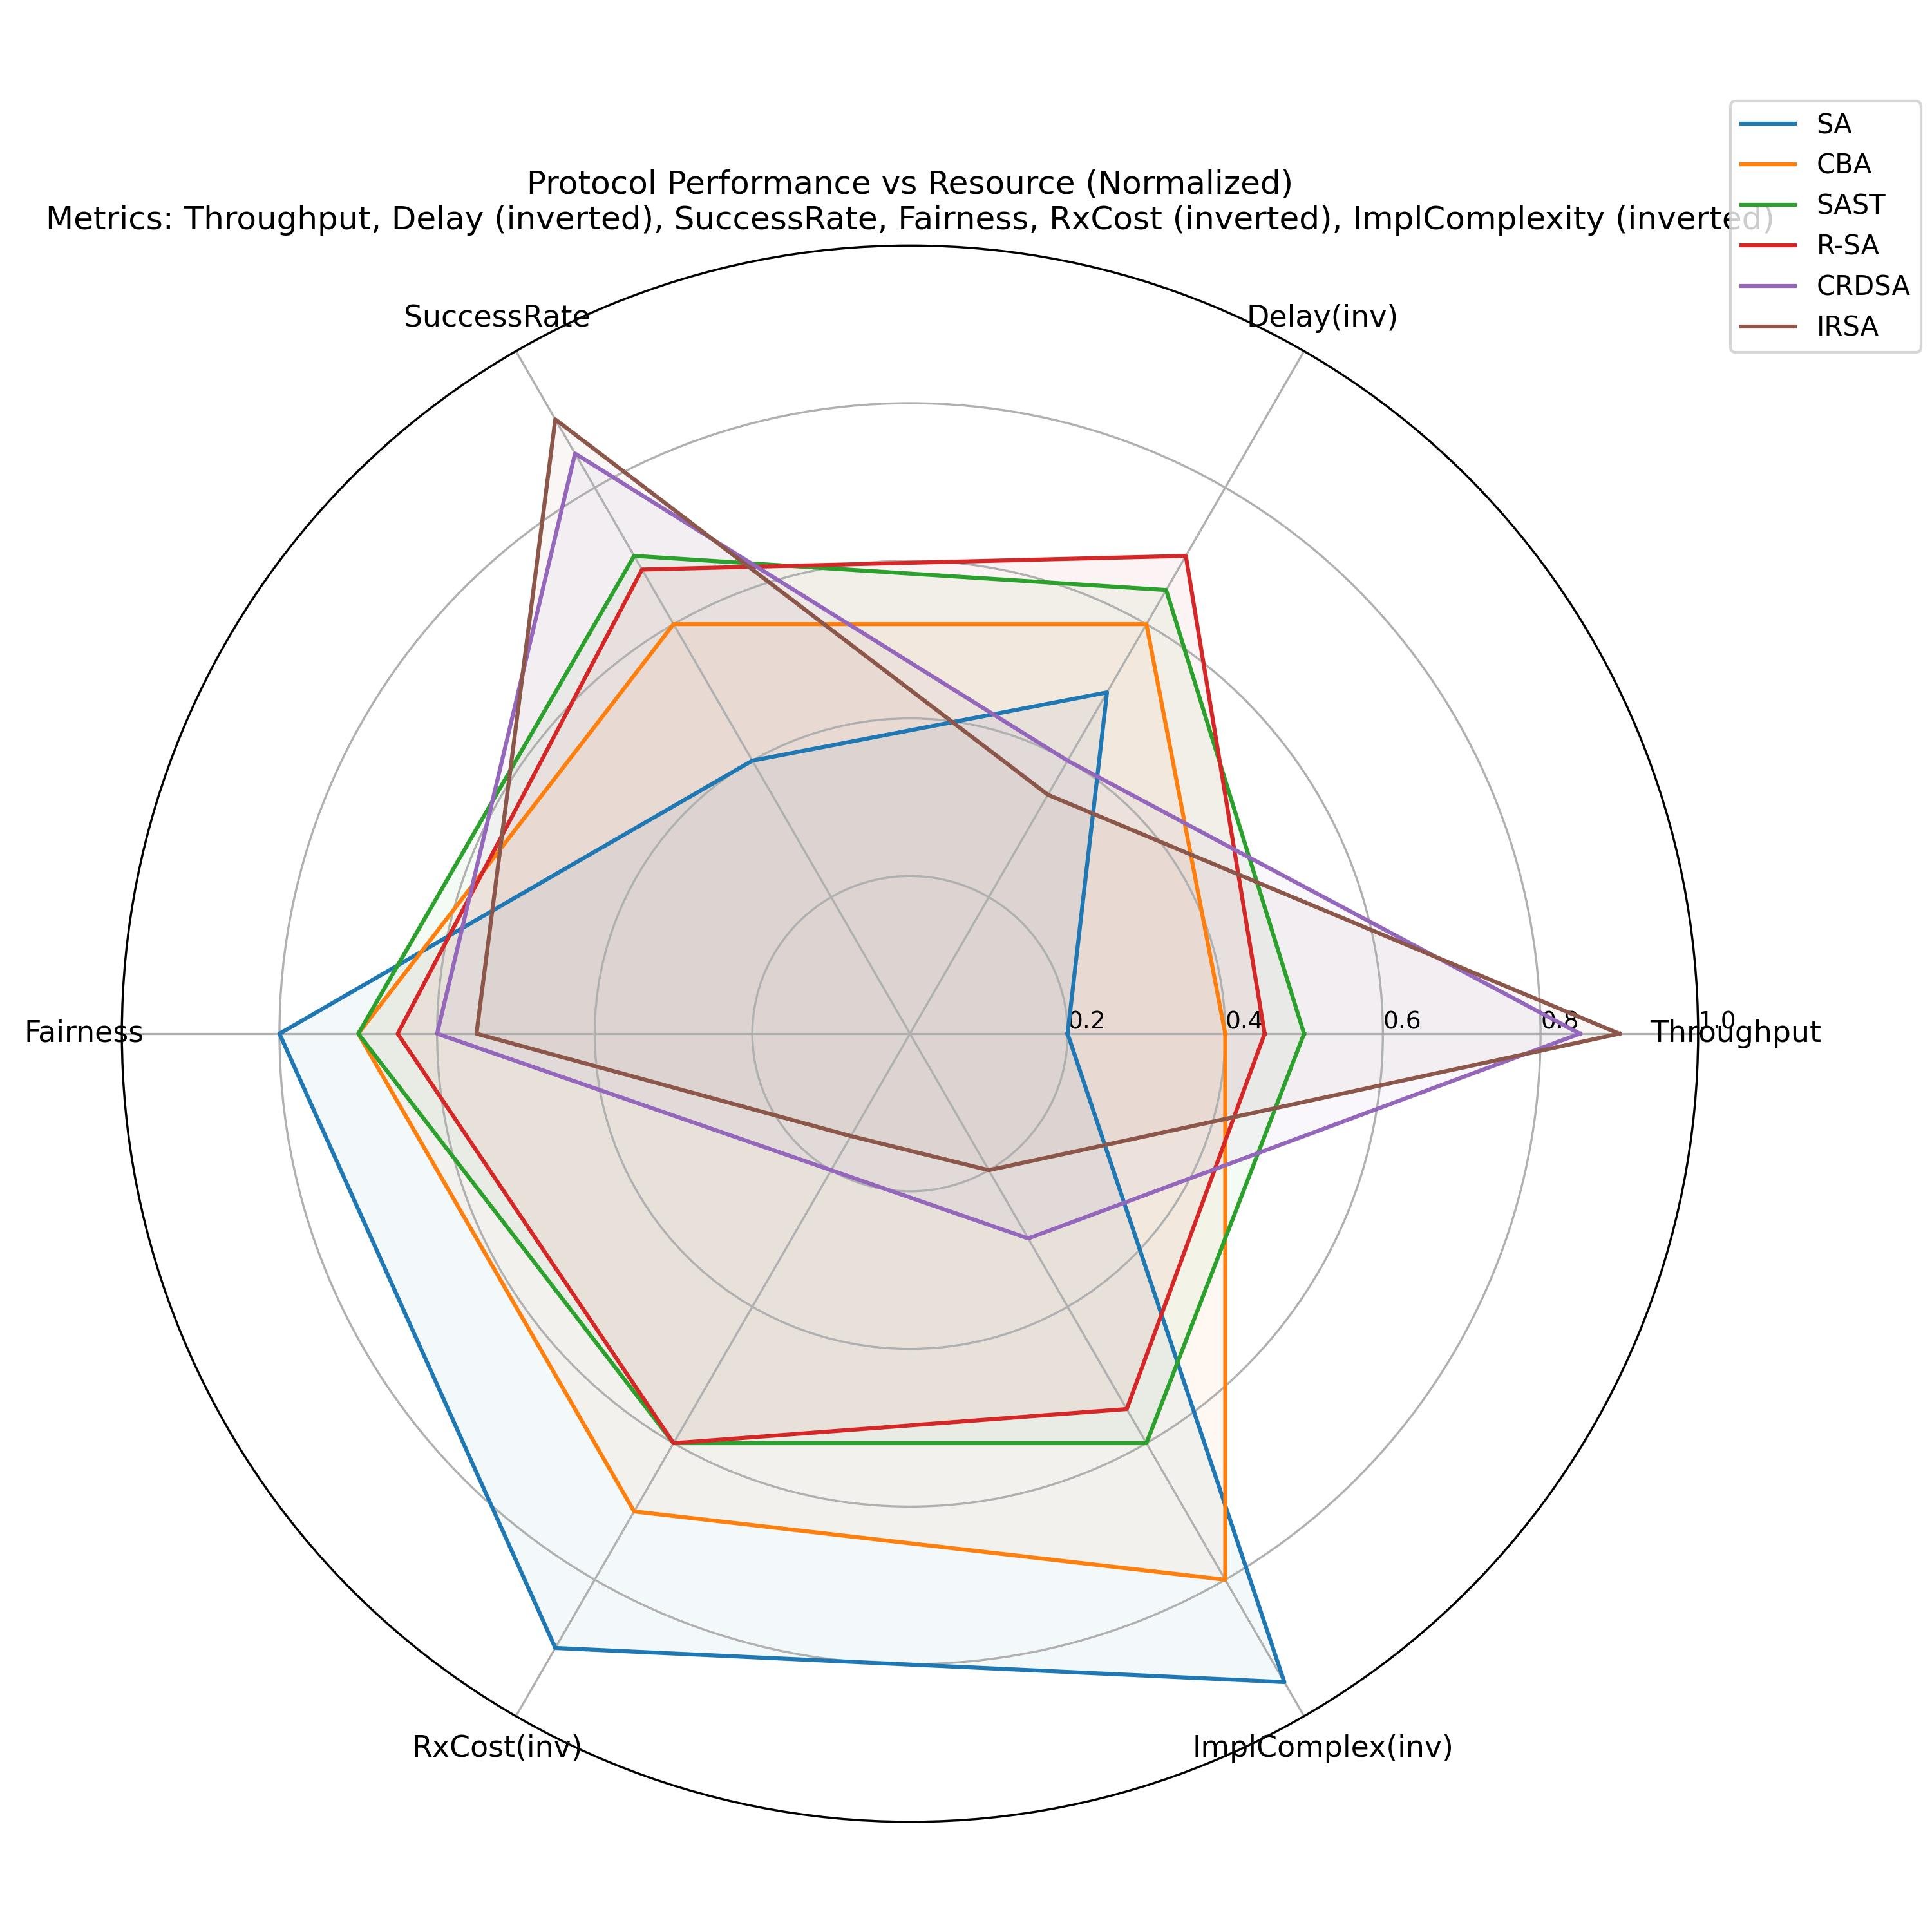
\includegraphics[width=0.3\textwidth]{figure/chap5/Sim43.jpg}
% 		\label{fig:protocol_utility_comparison3}
% 	}
% 	\caption{不同协议在传输概率变化下的综合效用对比（固定平均到达率为 $\hat{\lambda}=0.3$）。}
% 	\label{fig:protocol_utility_comparison}
% \end{figure}

% === 1. 将下列内容剪切到5.2.4节合适位置（如“仿真性能验证与对比”小节中） ===

% \subsection{不同\(\lambda\)下均匀流量场景的性能对比}
% 为进一步展示不同协议在均匀流量（uniform）场景下随接入概率\(q\)变化的性能差异，本文对\(\lambda=0.001, 0.003, 0.005, 0.01\)四种典型到达率下的时延、吞吐量、公平性、信令开销等指标进行了仿真对比，结果如下图所示。

% % 延迟对比
% \begin{figure}[htbp]
%     \centering
%     % 四个子图
%     \subfloat[$\lambda=0.01$]{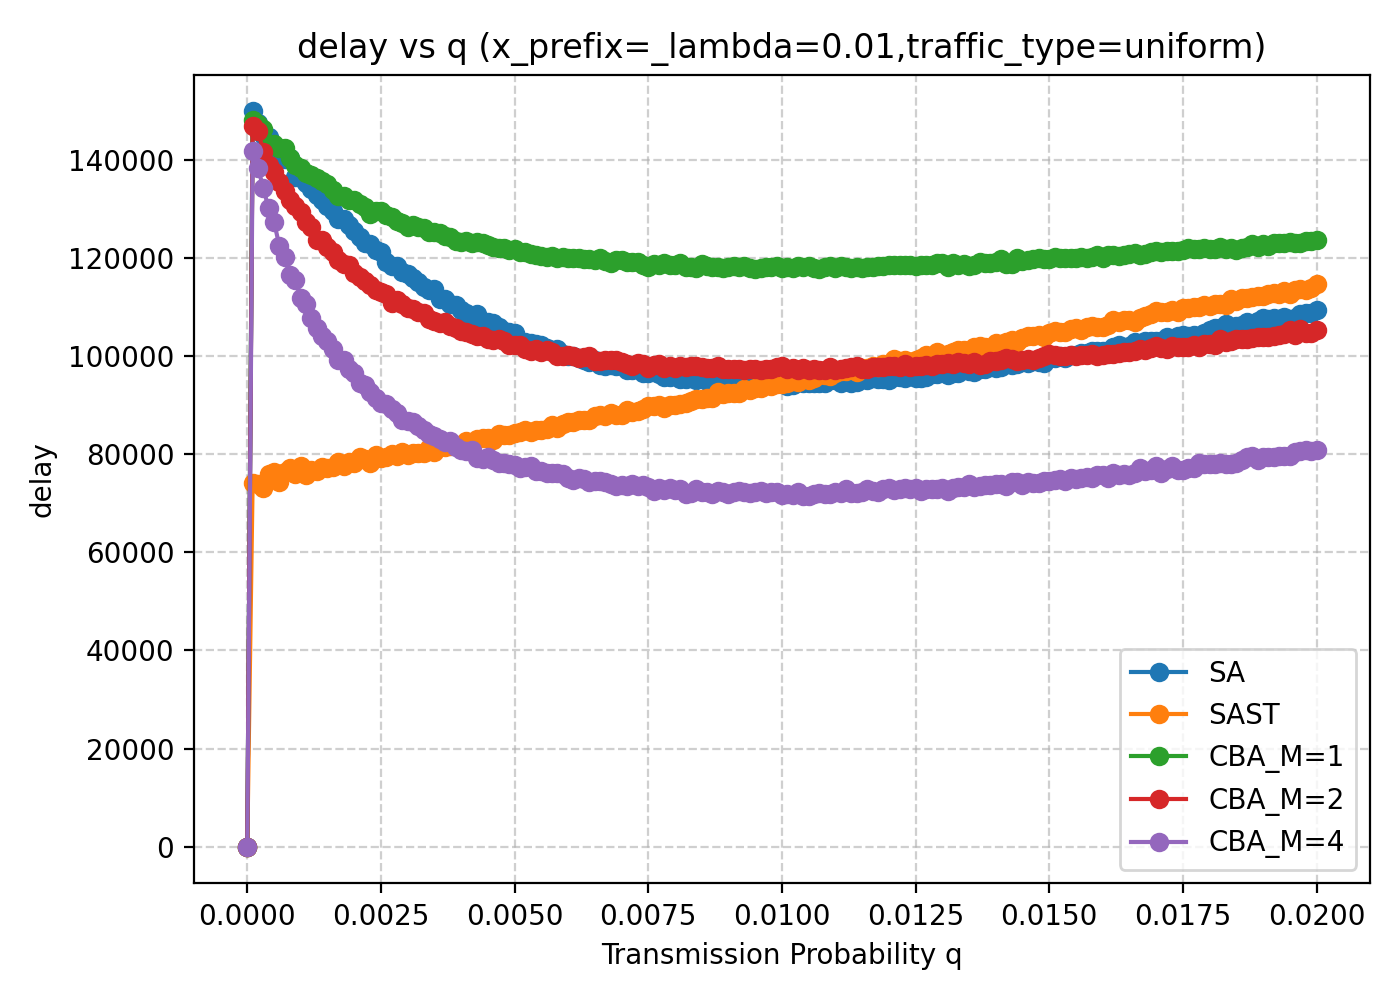
\includegraphics[width=0.24\textwidth]{figure/chap5/delay_vs_q_xprefix__lambda=0.01,traffic_type=uniform.pdf}}
%     \subfloat[$\lambda=0.001$]{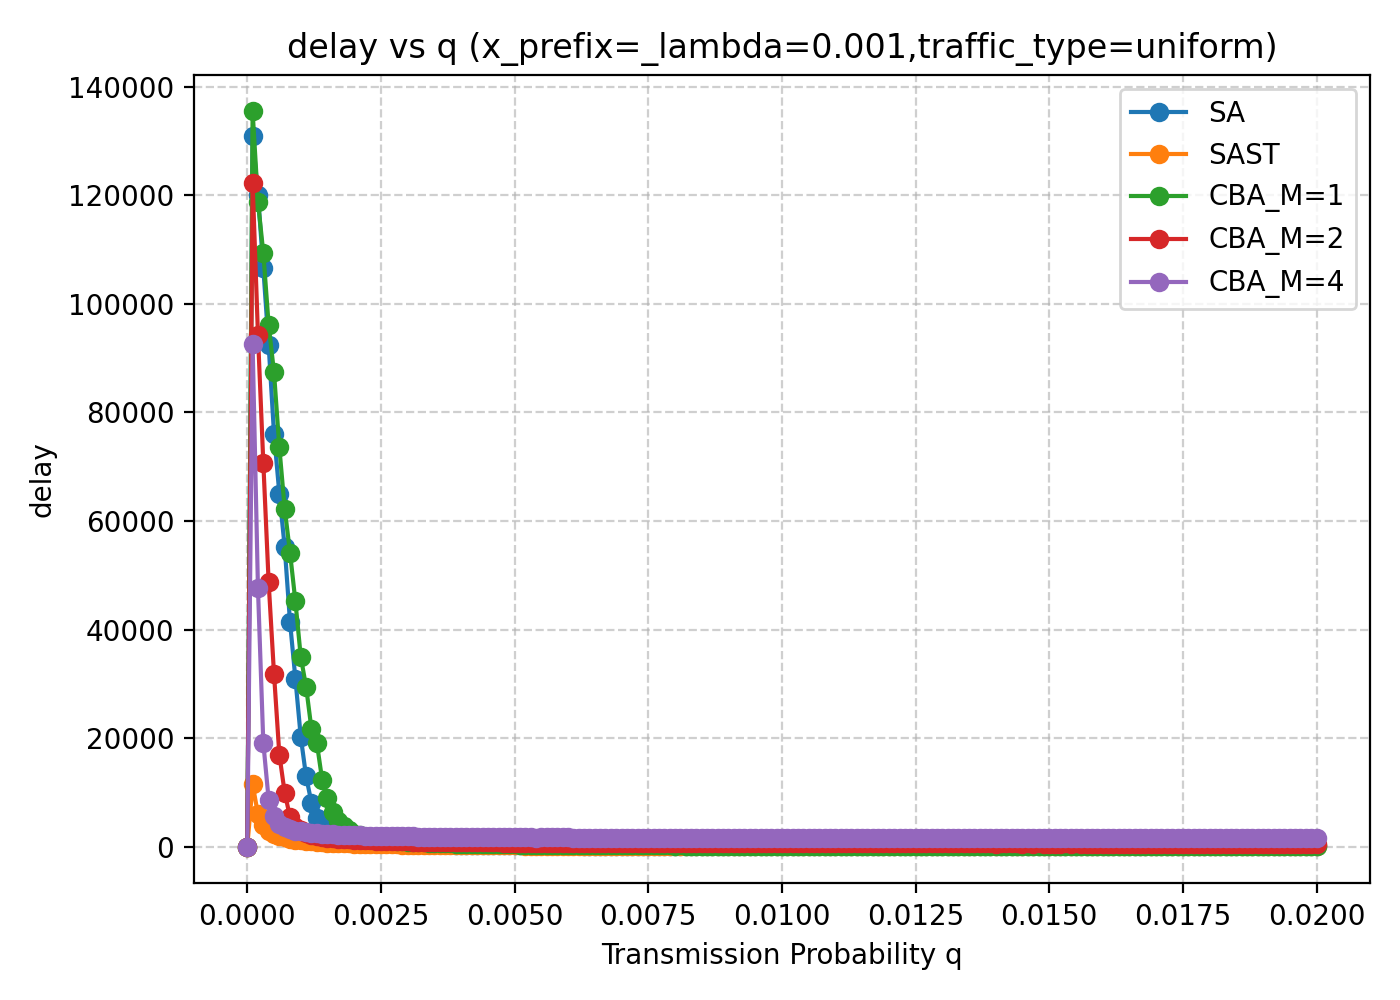
\includegraphics[width=0.24\textwidth]{figure/chap5/delay_vs_q_xprefix__lambda=0.001,traffic_type=uniform.pdf}}
%     \subfloat[$\lambda=0.003$]{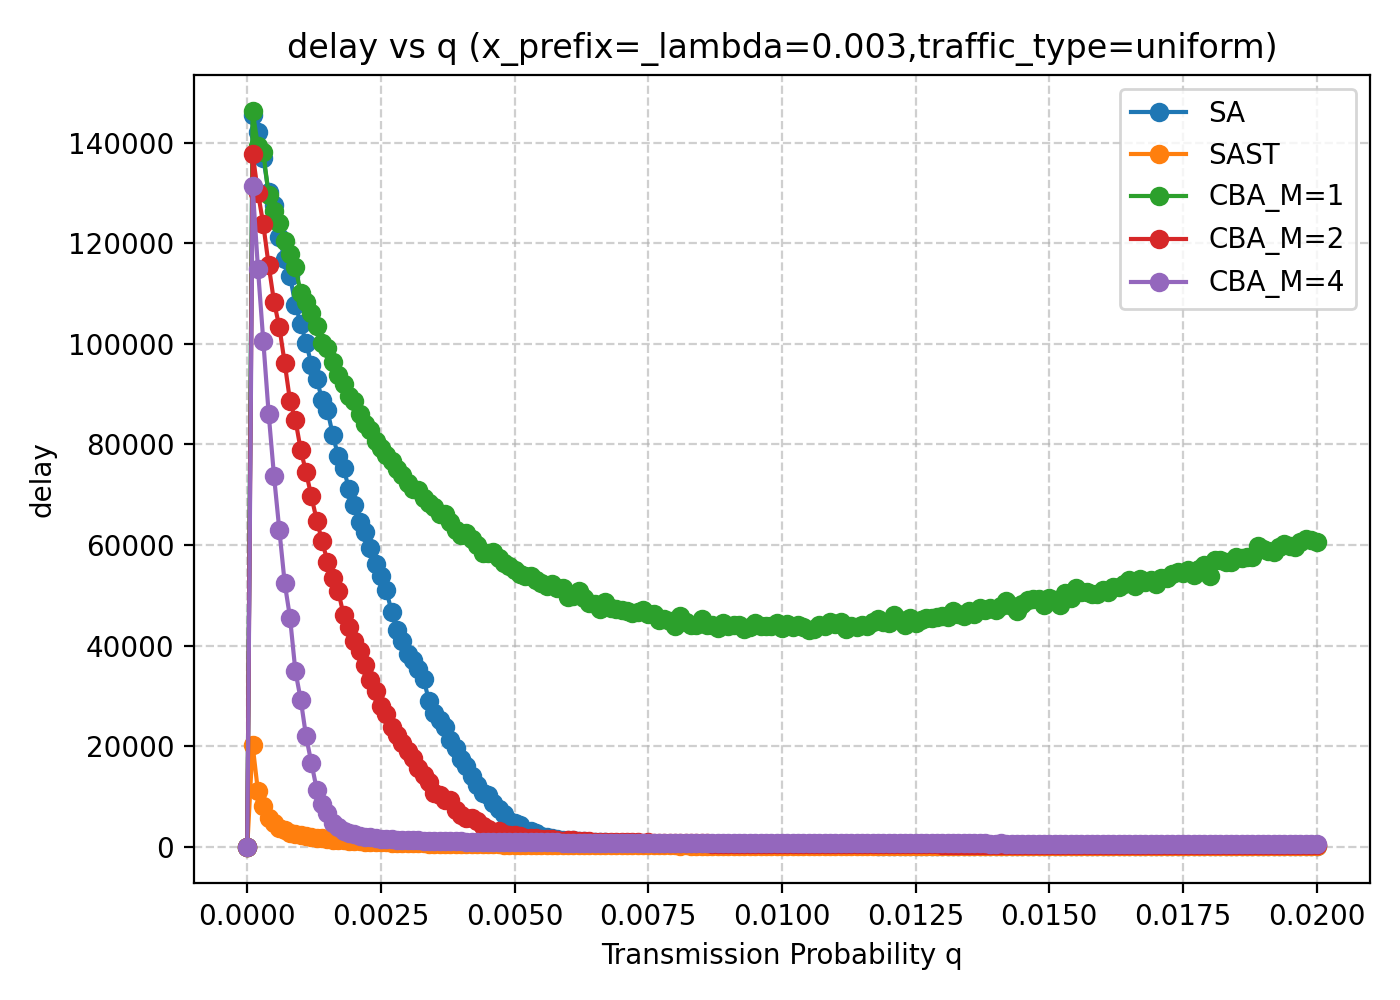
\includegraphics[width=0.24\textwidth]{figure/chap5/delay_vs_q_xprefix__lambda=0.003,traffic_type=uniform.pdf}}
%     \subfloat[$\lambda=0.005$]{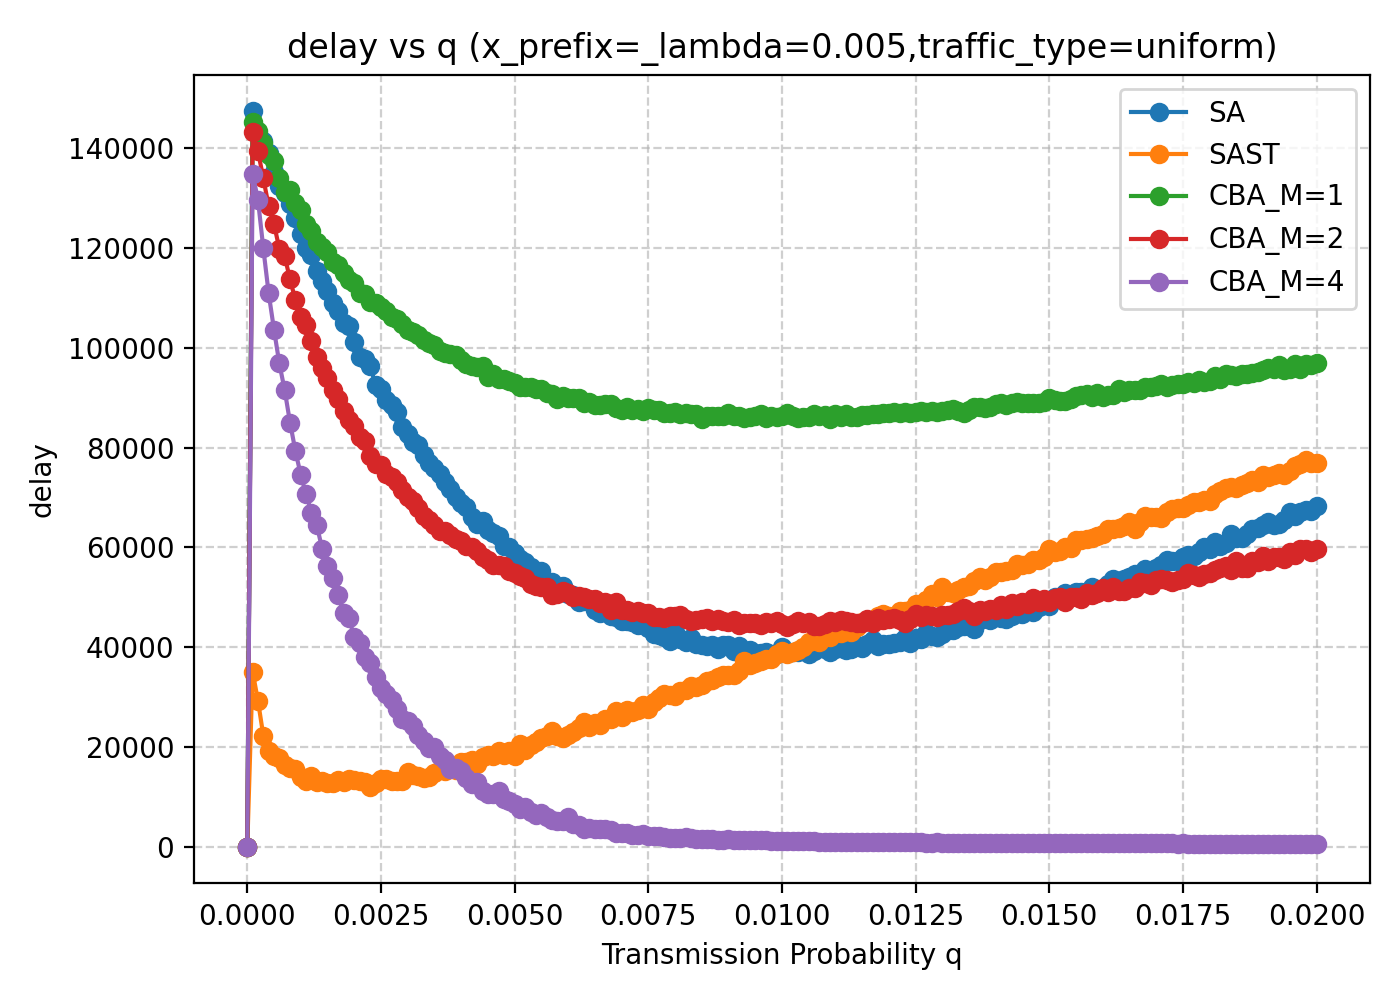
\includegraphics[width=0.24\textwidth]{figure/chap5/delay_vs_q_xprefix__lambda=0.005,traffic_type=uniform.pdf}}
%     \caption{不同$\lambda$下均匀流量场景的平均时延$D$随$q$变化对比}
%     \label{fig:delay_vs_q_uniform}
% \end{figure}

% % 公平性对比
% \begin{figure}[htbp]
%     \centering
%     \subfloat[$\lambda=0.01$]{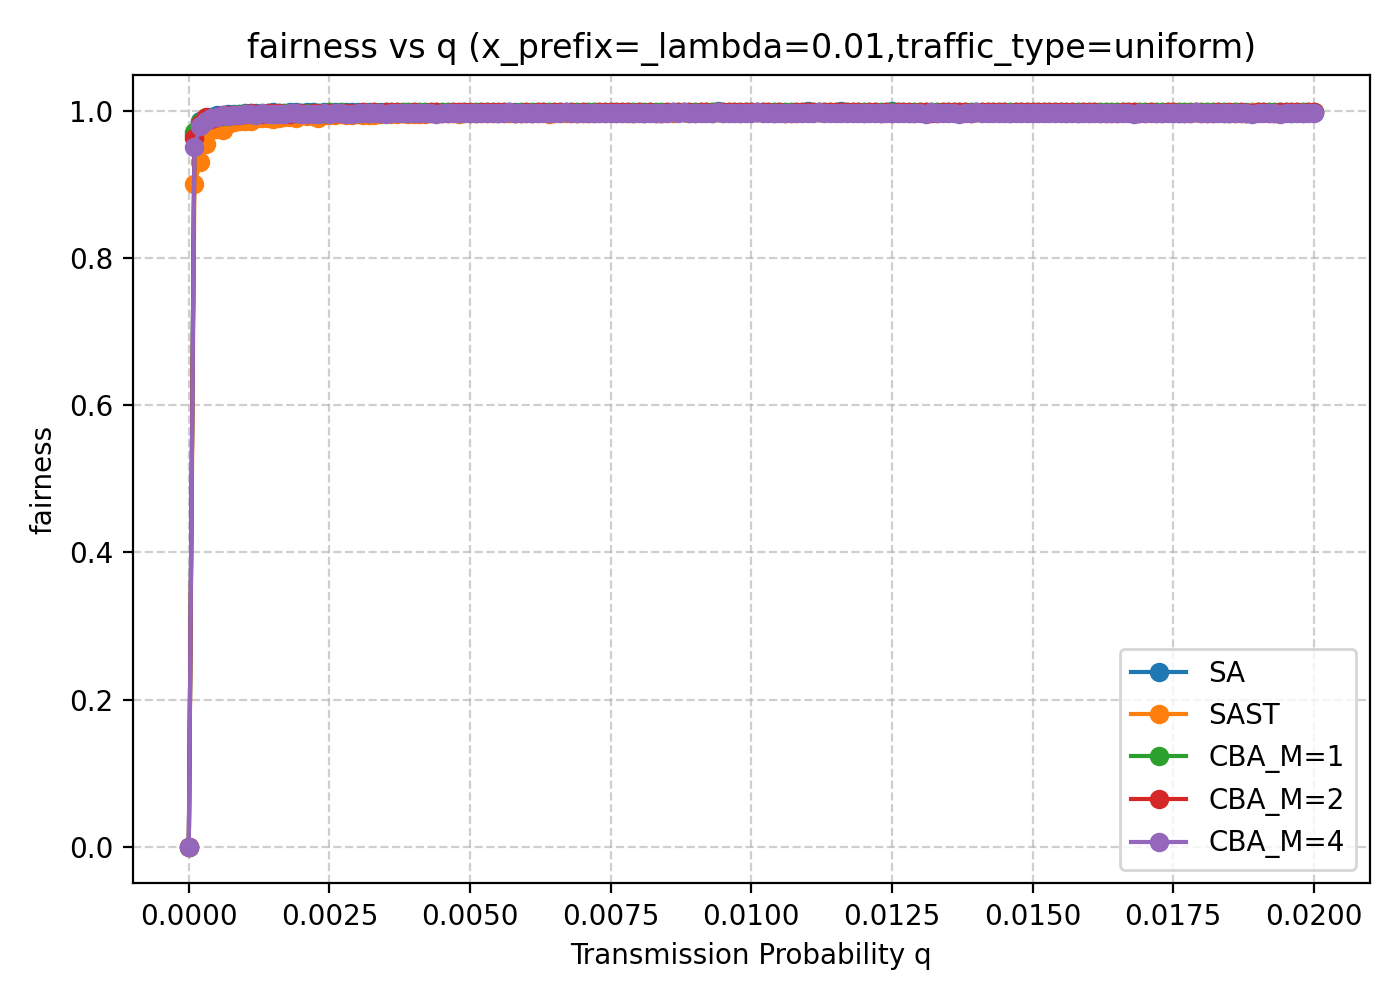
\includegraphics[width=0.24\textwidth]{figure/chap5/fairness_vs_q_xprefix__lambda=0.01,traffic_type=uniform.pdf}}
%     \subfloat[$\lambda=0.001$]{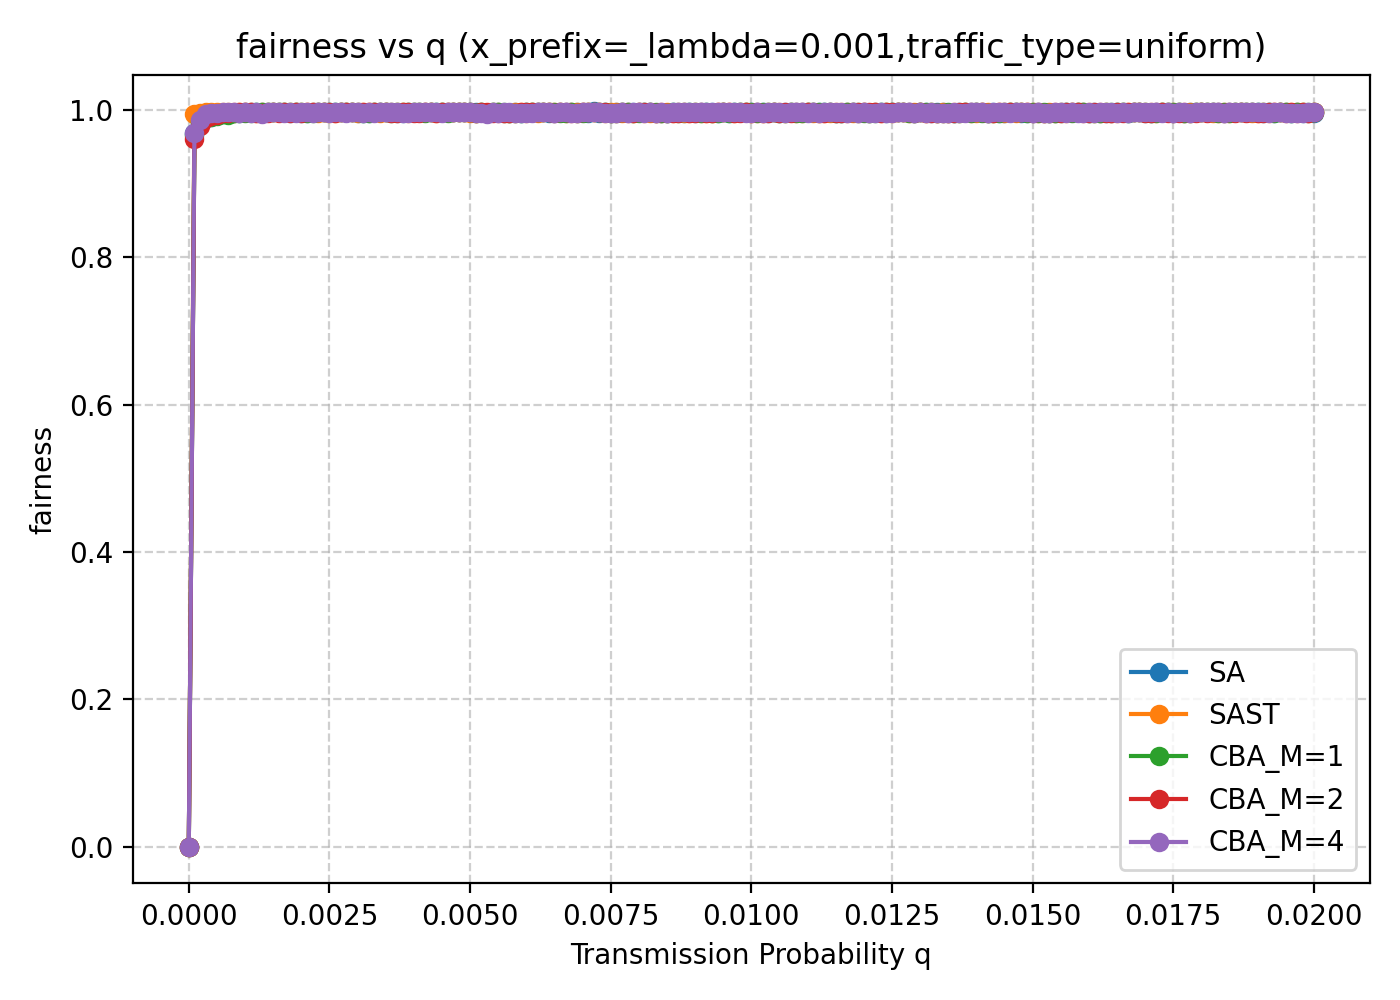
\includegraphics[width=0.24\textwidth]{figure/chap5/fairness_vs_q_xprefix__lambda=0.001,traffic_type=uniform.pdf}}
%     \subfloat[$\lambda=0.003$]{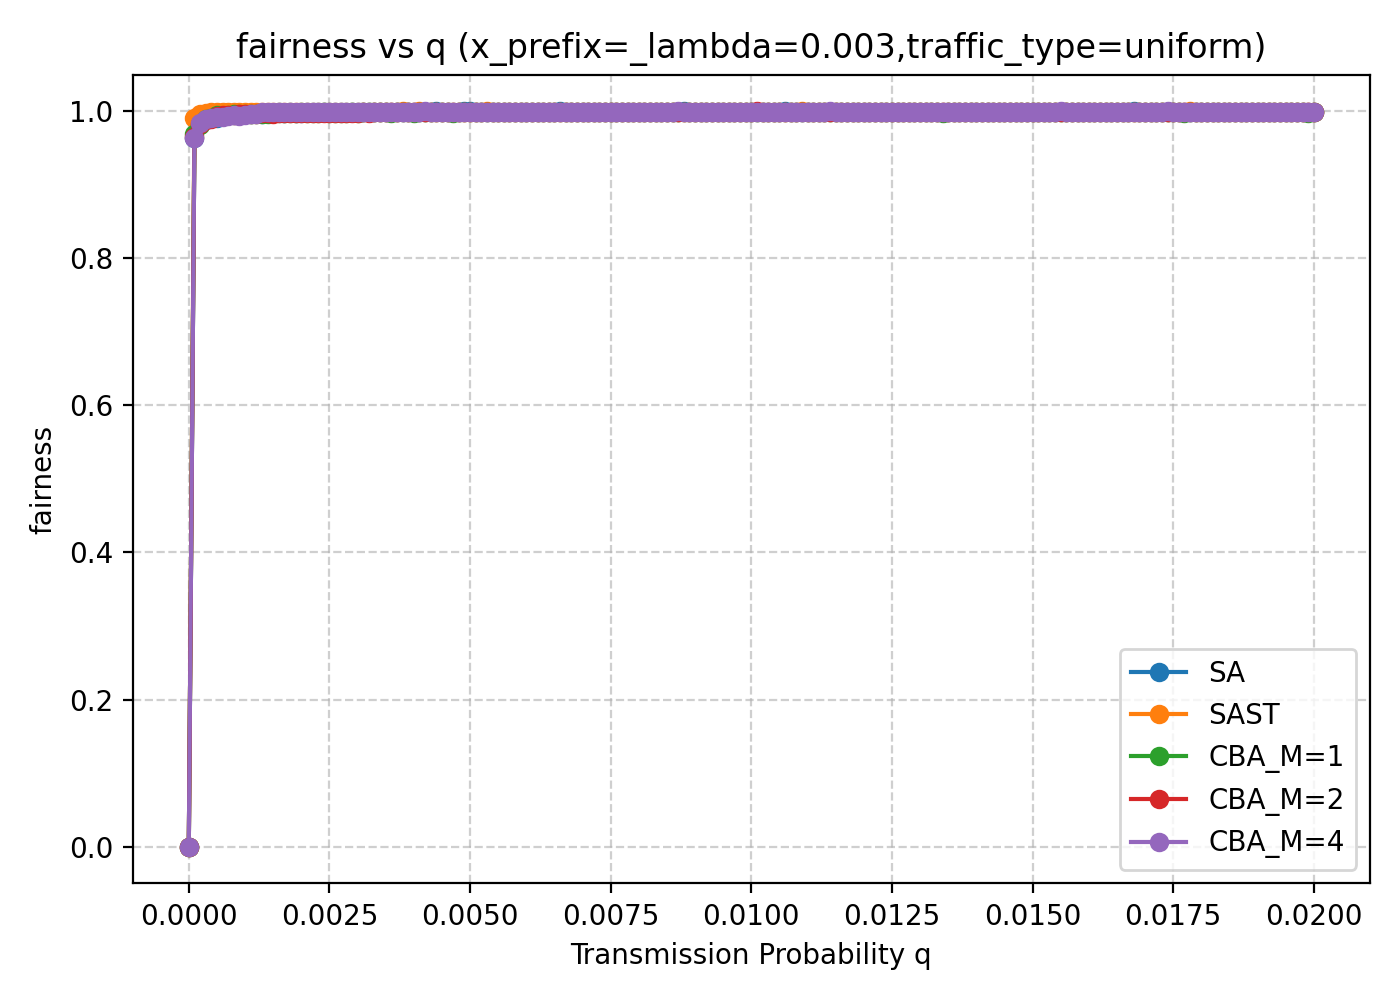
\includegraphics[width=0.24\textwidth]{figure/chap5/fairness_vs_q_xprefix__lambda=0.003,traffic_type=uniform.pdf}}
%     \subfloat[$\lambda=0.005$]{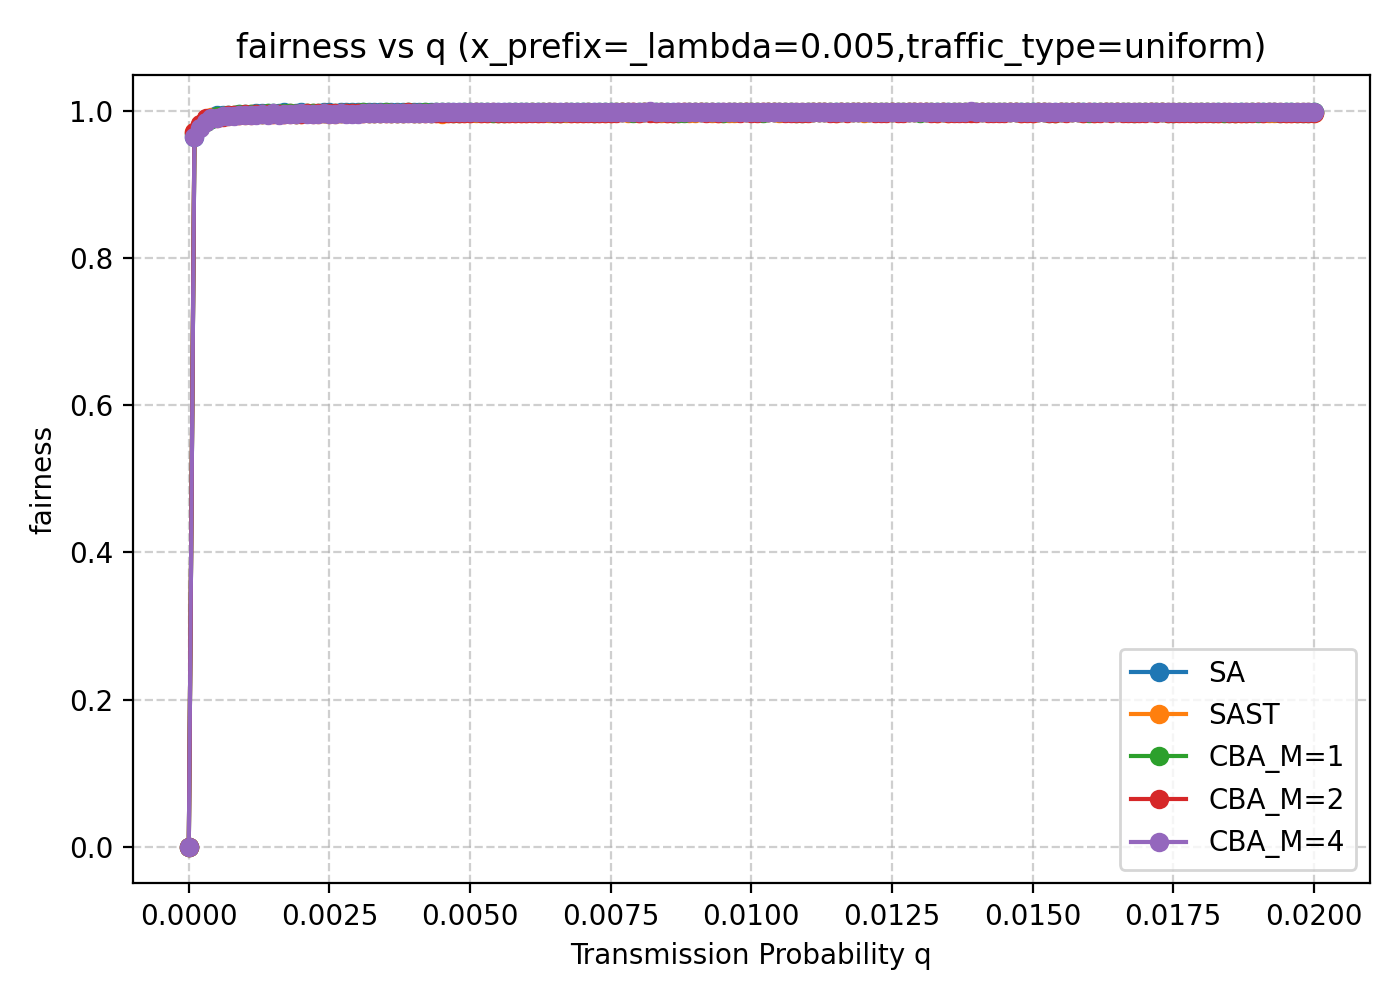
\includegraphics[width=0.24\textwidth]{figure/chap5/fairness_vs_q_xprefix__lambda=0.005,traffic_type=uniform.pdf}}
%     \caption{不同$\lambda$下均匀流量场景的公平性$J_T$随$q$变化对比}
%     \label{fig:fairness_vs_q_uniform}
% \end{figure}

% % 信令开销对比
% \begin{figure}[htbp]
%     \centering
%     \subfloat[$\lambda=0.01$]{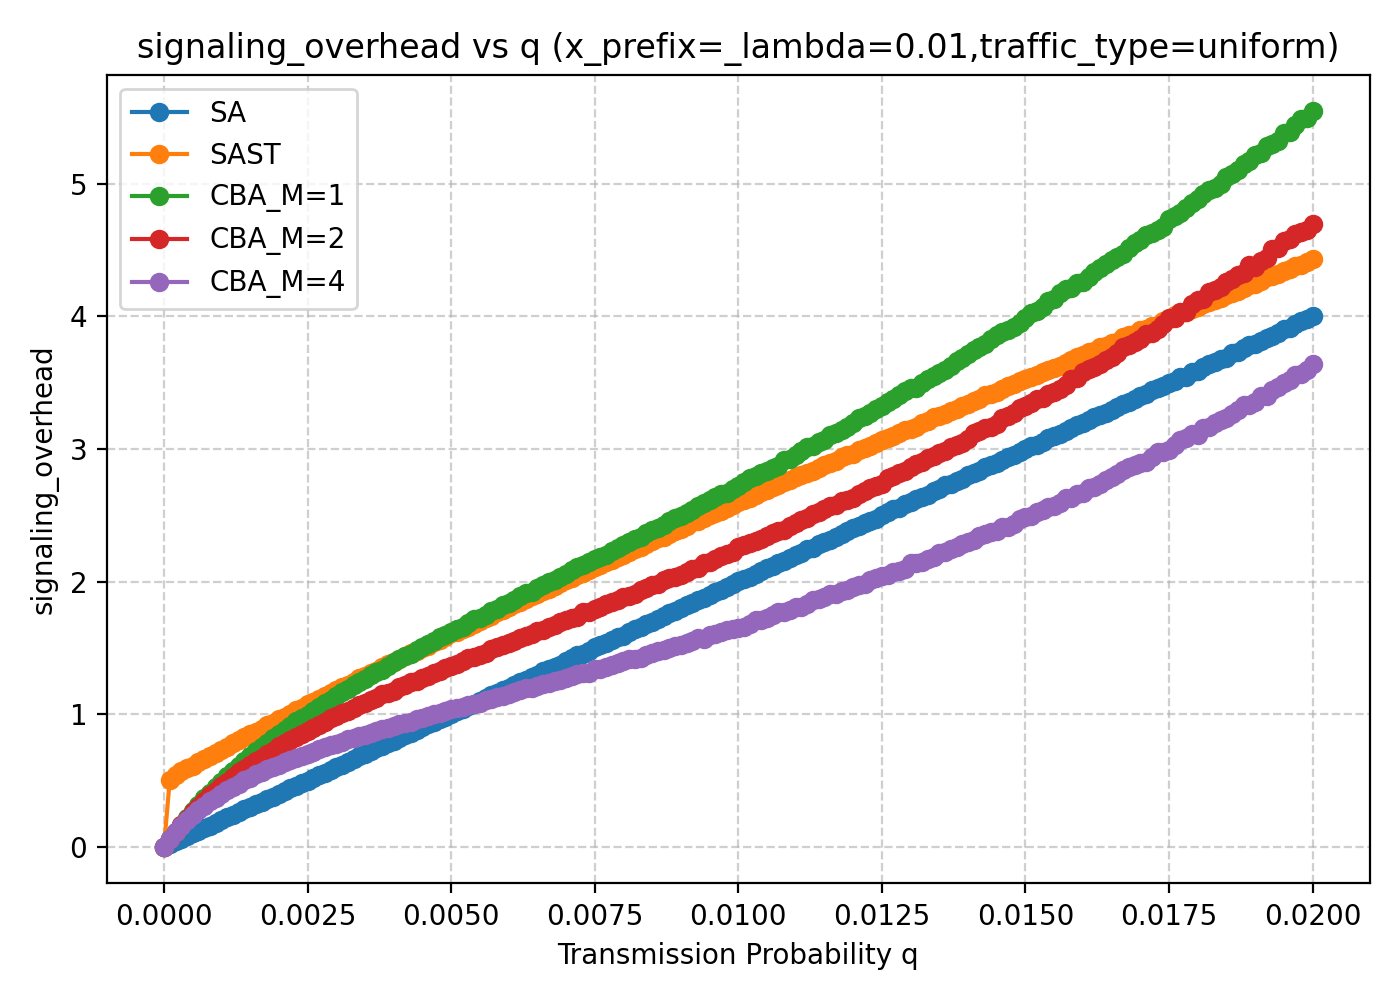
\includegraphics[width=0.24\textwidth]{figure/chap5/signaling_overhead_vs_q_xprefix__lambda=0.01,traffic_type=uniform.pdf}}
%     \subfloat[$\lambda=0.001$]{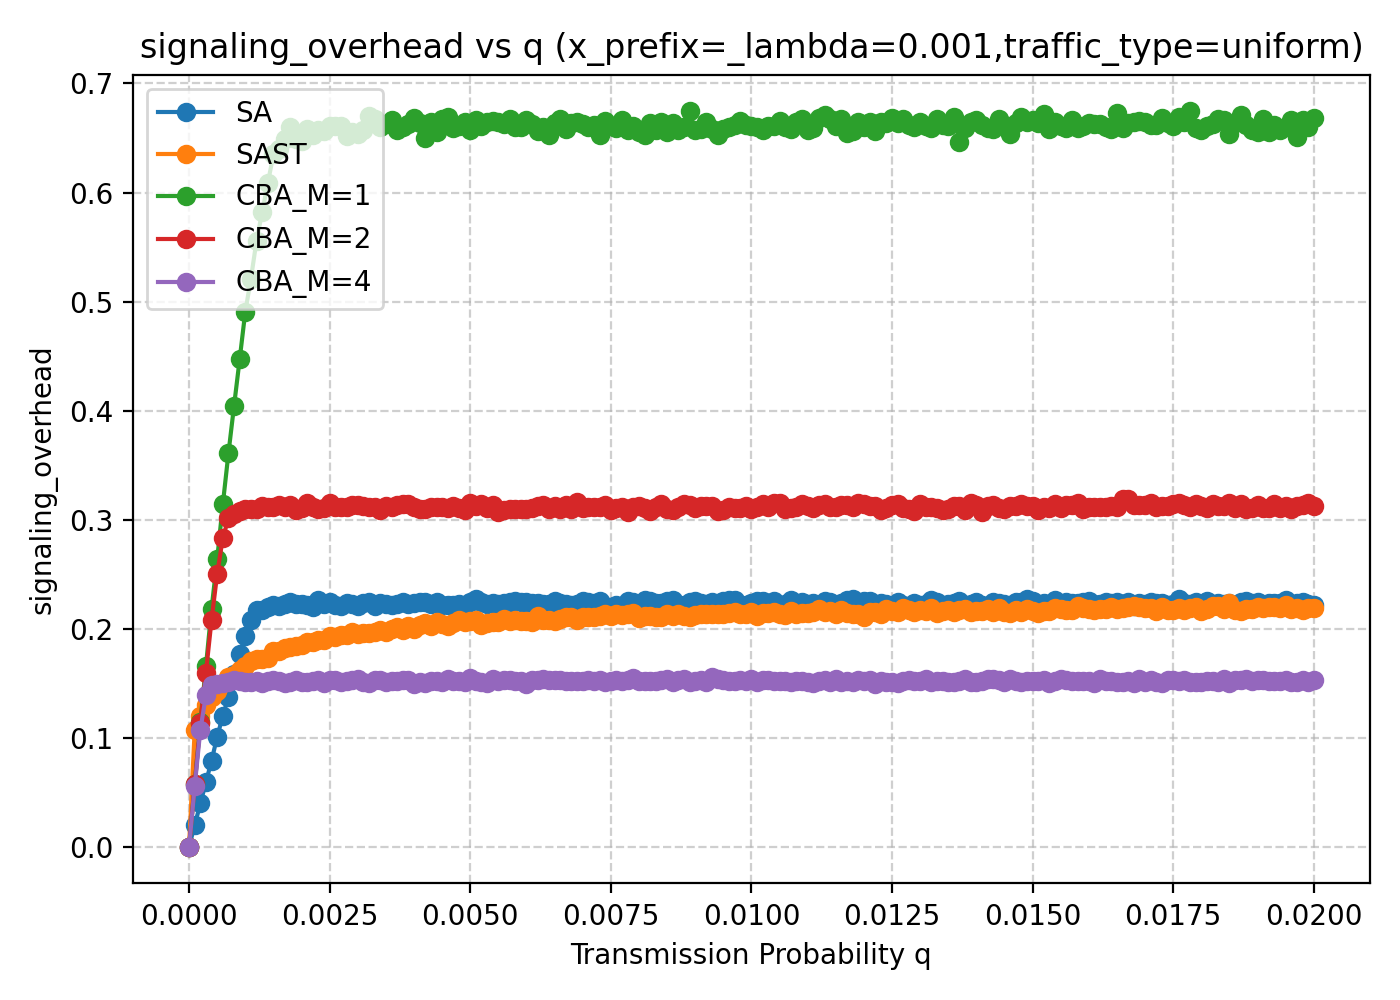
\includegraphics[width=0.24\textwidth]{figure/chap5/signaling_overhead_vs_q_xprefix__lambda=0.001,traffic_type=uniform.pdf}}
%     \subfloat[$\lambda=0.003$]{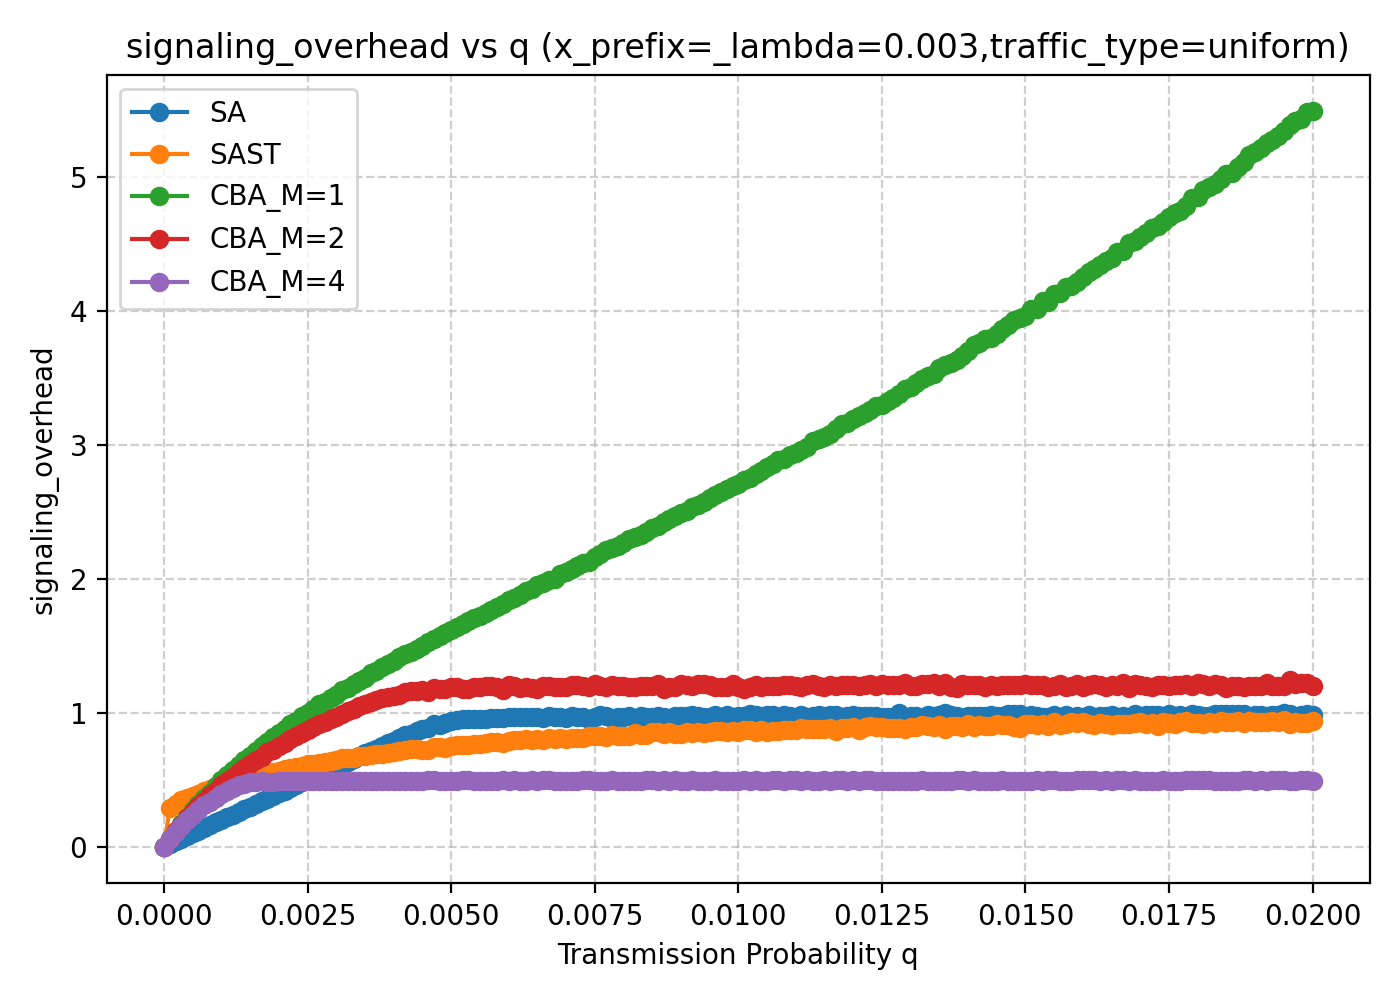
\includegraphics[width=0.24\textwidth]{figure/chap5/signaling_overhead_vs_q_xprefix__lambda=0.003,traffic_type=uniform.pdf}}
%     \subfloat[$\lambda=0.005$]{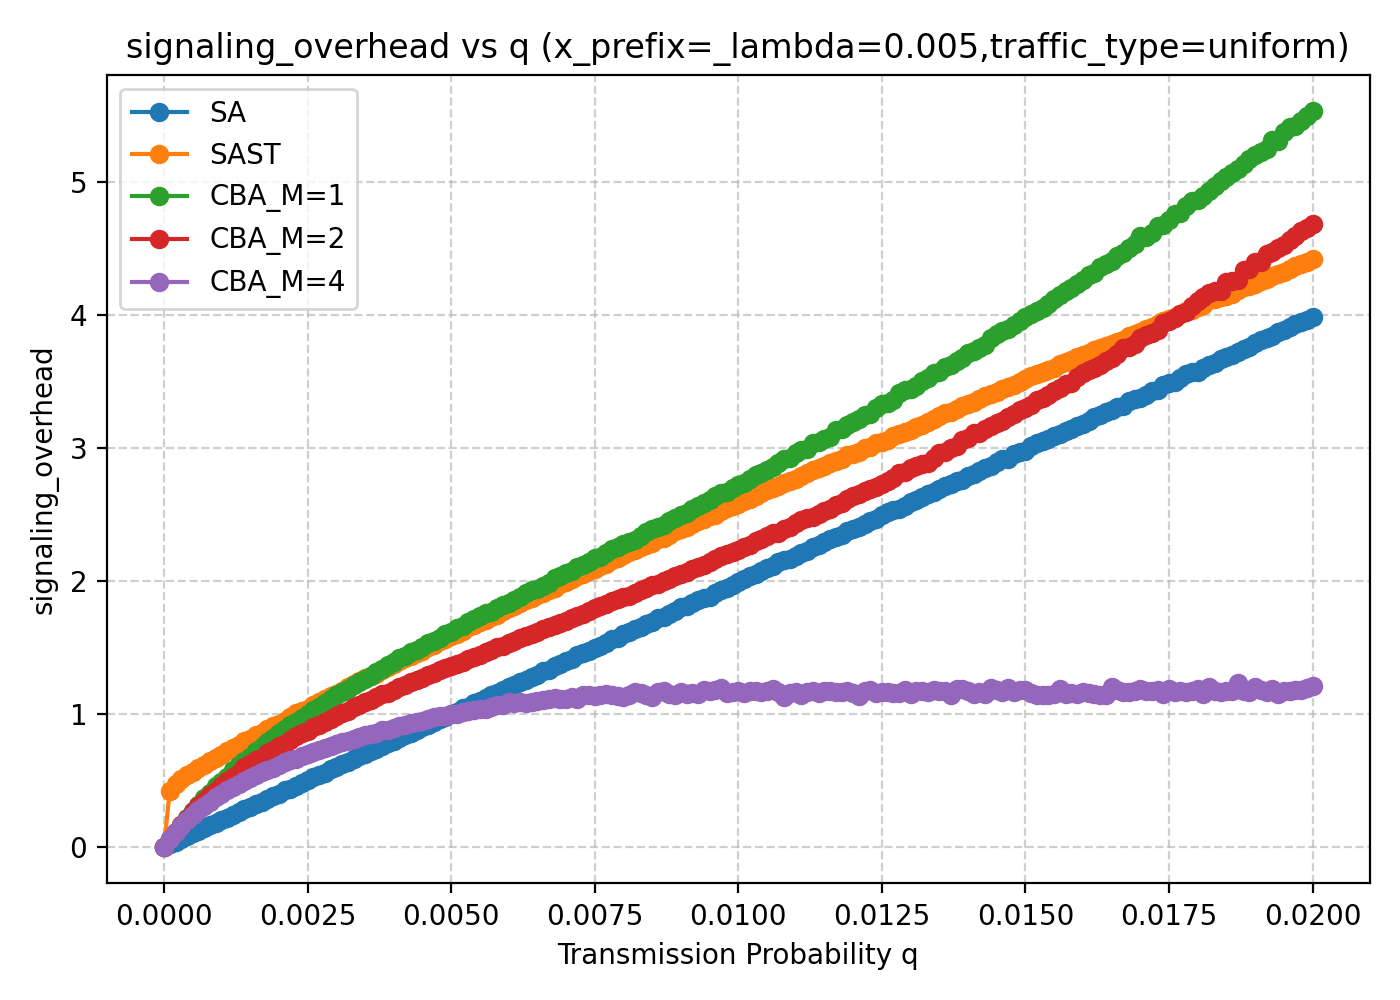
\includegraphics[width=0.24\textwidth]{figure/chap5/signaling_overhead_vs_q_xprefix__lambda=0.005,traffic_type=uniform.pdf}}
%     \caption{不同$\lambda$下均匀流量场景的信令开销$S$随$q$变化对比}
%     \label{fig:signaling_vs_q_uniform}
% \end{figure}


% 上述结果直观展现了在不同流量强度下，三类协议在主要性能指标上的变化趋势，为后续协议选择与参数优化提供了数据支撑。

% === 2. 小结部分只保留简要总结，不再重复上述仿真结果 ===

% =========================================================
% 第 5.3 节：基于多任务深度学习的性能预测模型
% =========================================================

\section{基于多任务深度学习的性能预测模型}
\label{sec:mt_dnn_model}

离散事件仿真器能够在给定协议配置和网络条件下精确评估系统性能，但其计算开销较高。以典型仿真配置（如 $n=100$ 个节点、$T=3\times10^5$ 个时隙）为例，单次样本点的仿真通常需要数十秒甚至数分钟。当需要在多协议、多参数组合及不同流量场景下进行大规模性能评估时，总体仿真时间将迅速累积。本节基于第\ref{subsec:dataset_construction}节构建的仿真数据集，设计并训练一种高效的多任务性能预测模型（Multi-Task Deep Neural Network, MT-DNN）。后文统一简称为性能预测模型。该模型通过共享特征表示并联合学习多个性能指标，实现对系统吞吐量、时延与公平性等关键指标的快速预测。相比传统仿真方法，该模型能够将性能评估时间从分钟级显著降低至毫秒级，从而为后续的协议选择与参数优化提供高效支撑。

\subsection{基于硬参数共享的多任务网络架构}
\label{subsec:hard_sharing}

考虑到网络性能指标之间存在显著的物理耦合性，例如高负载状态通常同时对应吞吐量饱和与时延激增，独立的单任务模型往往忽略了这些内在关联，且训练效率低下。为此，本文设计了基于硬参数共享机制的神经网络架构，该架构在保持参数量可控的同时，能够有效学习多任务间的关联。

\paragraph{架构设计原理}
硬参数共享架构由以下三个核心模块组成：
\begin{itemize}[leftmargin=*]
	\item \textbf{输入归一化层}：采用 LayerNorm 对输入特征进行归一化，消除不同特征量纲差异，稳定梯度流。
	\item \textbf{共享特征提取层}：由两至三层全连接网络堆叠而成，每层均配备 LayerNorm、GELU 激活函数和 Dropout。该部分负责提取所有任务通用的网络状态表征。
	\item \textbf{任务特定头部}：针对每个任务设置独立的单层线性映射，实现从共享特征到任务输出的最终转换。
\end{itemize}

网络的数学描述如下。设输入特征维度为 $D_{\text{in}}$，共享层隐藏维度为 $D_{\text{hidden}}$，共享层深度为 $L$。首先对输入特征与掩码向量逐元素相乘并归一化：
\begin{equation}
	\mathbf{h}^{(0)} = \text{LayerNorm}(\mathbf{X}_{\text{in}} \odot \mathbf{m})
\end{equation}
其中 $\mathbf{m}$ 为掩码向量，用于屏蔽无效参数分量。随后依次进行特征变换和非线性映射：
\begin{equation}
	\mathbf{h}^{(\ell)} = \text{Dropout}\left( \sigma\left( \text{LayerNorm}(\mathbf{W}^{(\ell)} \mathbf{h}^{(\ell-1)} + \mathbf{b}^{(\ell)}) \right) \right), \quad \ell = 1, \ldots, L
\end{equation}
其中 $\sigma$ 表示 GELU 激活函数，Dropout 比率为 0.1。对于第 $k$ 个任务，输出通过线性映射获得：
\begin{equation}
	\hat{y}_k = \mathbf{w}_k \cdot \mathbf{h}^{(L)} + b_k
\end{equation}
各任务输出为连续值，无需额外激活函数。

\begin{table}[htbp]
	\centering
	\caption{多任务性能预测模型的神经网络架构}
	\label{tab:nn_architecture}
	\renewcommand{\arraystretch}{1.25}
	\begin{tabular}{lll}
		\toprule
		\textbf{模块} & \textbf{结构配置} & \textbf{参数说明} \\
		\midrule
		\multirow{2}{*}{输入层} 
		& LayerNorm 
		& 特征归一化以稳定训练过程 \\
		& 掩码乘法 
		& $\mathbf{X}_{\mathrm{in}} \odot \mathbf{m}$，屏蔽无效或缺失特征 \\
		\midrule
		\multirow{5}{*}{共享隐藏层} 
		& FC + LayerNorm 
		& 维度映射 $D_{\mathrm{in}} \rightarrow D_{\mathrm{hidden}}$（如 128） \\
		& GELU + Dropout 
		& 非线性激活与正则化，Dropout 概率 $p=0.1$ \\
		& FC + LayerNorm 
		& 隐藏层维度保持 $D_{\mathrm{hidden}} \rightarrow D_{\mathrm{hidden}}$ \\
		& GELU + Dropout 
		& 激活与正则化 \\
		& 可选第 3 层
		& 深层模式下启用，用于提升模型表达能力 \\
		\midrule
		\multirow{2}{*}{任务输出头} 
		& 每任务独立全连接层 
		& 输出维度为 1 \\
		& 无激活函数 
		& 回归任务，直接输出连续值 \\
		\bottomrule
	\end{tabular}
\end{table}

\begin{figure}[t]
	\centering
	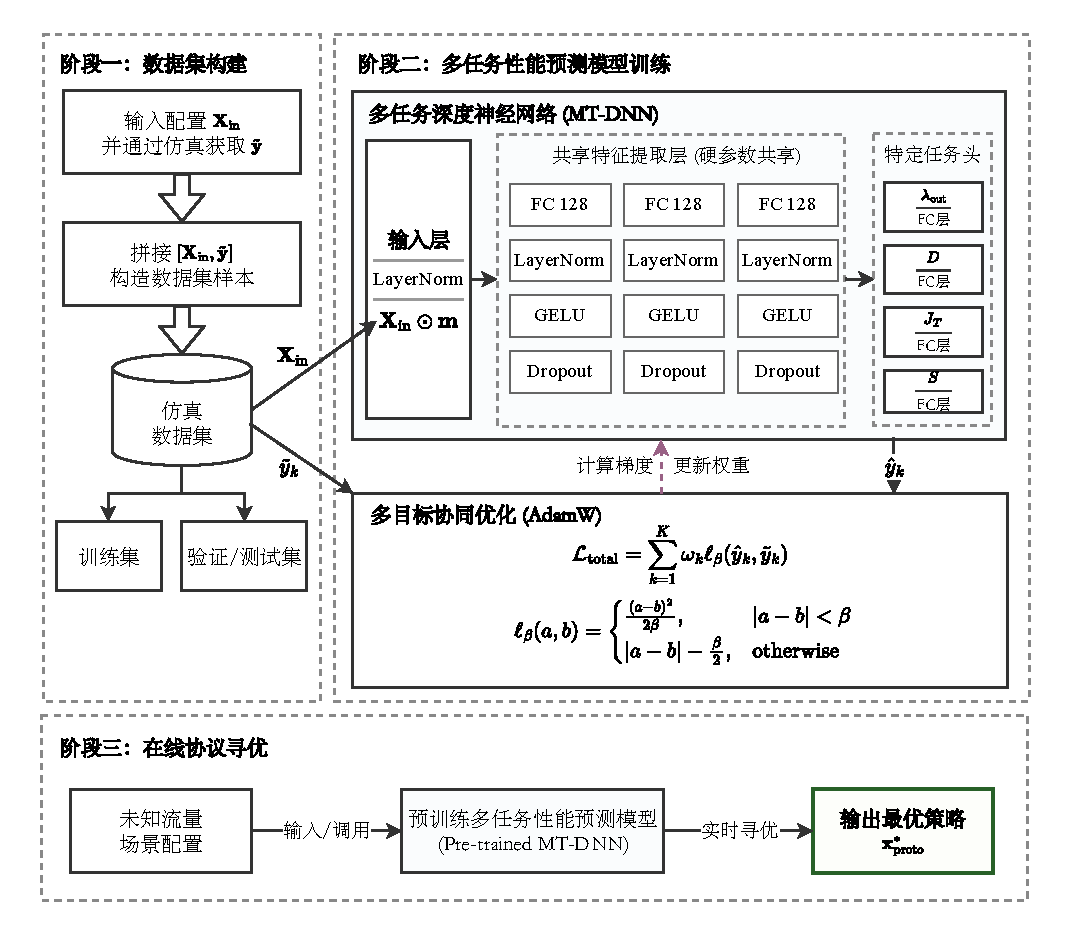
\includegraphics[width=0.95\textwidth]{figure/chap5/神经网络训练流程.pdf}
	\caption{多任务性能预测模型的训练流程示意图}
	\label{fig:nn_training_flow}
\end{figure}

图~\ref{fig:nn_training_flow} 给出多任务性能预测模型的训练流程，包括数据预处理、特征归一化、前向传播、多任务损失计算、参数优化与验证集监控等环节。在标准配置下，模型输入特征维度约为 14，隐藏层宽度为 256，输出端包含 4 个任务分支，参数量约为 71,712--138,016（对应浅层/深层两种结构）。结合前述数据集规模，训练样本量与参数量之比约为 0.086--0.165，可用于评估模型复杂度与样本规模的匹配程度。

\subsection{多目标协同优化与训练策略}
\label{subsec:training}


在多任务学习框架中，不同预测目标通常具有不同的数值尺度与优化难度。若将各任务损失直接等权叠加，梯度更新容易被尺度较大的任务主导，进而削弱对其他关键指标的学习效果。为实现吞吐量、时延、公平性与信令开销四类指标的协同预测，本文采用统一训练策略，将多任务损失建模、正则化约束与自适应优化结合，以提升训练稳定性与泛化能力。

在训练目标设计方面，本文对输入特征采用标准化处理，对输出标签采用最小-最大归一化处理，并将时延指标先进行对数变换以缓解长尾分布影响。在此基础上，采用加权 Smooth L1 作为总体优化目标：
\begin{equation}
\mathcal{L}_{\text{total}}
=
\sum_{k=1}^{K}
\omega_k\,
\ell_{\beta}\!\left(\hat{y}_k,\tilde{y}_k\right),
\end{equation}
其中
\begin{equation}
\ell_{\beta}(a,b)=
\begin{cases}
\dfrac{(a-b)^2}{2\beta}, & |a-b|<\beta,\\[4pt]
|a-b|-\dfrac{\beta}{2}, & \text{otherwise}.
\end{cases}
\end{equation}
式中，$\tilde{y}_k$ 为归一化后的真实标签，$\hat{y}_k$ 为模型预测值，$\omega_k$ 为任务权重系数。本文标准配置下任务权重设置为 $(1,\,3,\,1,\,0.5)$，用于强调时延预测精度并对信令开销施加适度约束，从而实现性能指标与资源开销之间的平衡。

在模型泛化能力提升方面，本文在网络结构中引入 Dropout 与权重衰减，并在反向传播阶段采用梯度裁剪抑制梯度异常，提升深层网络训练的数值稳定性。输入扰动增强机制在框架中已实现，可用于模拟测量噪声与环境不确定性；在本文标准配置中该项默认关闭，以保证基线实验的可重复性与对比公平性。

在模型优化过程中，采用 AdamW 优化器进行端到端参数更新，并结合 ReduceLROnPlateau 学习率调度策略。当验证集指标在设定耐心周期内未见改善时，学习率按比例自动衰减以促进收敛；同时通过早停机制终止无效训练并保留最优参数。模型选择以验证集最大 MAE 为准，并设置目标阈值以实现精度驱动的提前停止，从而在训练效率与泛化性能之间取得平衡。


\subsection{性能预测模型的可视化结果}


\begin{table}[t]
\centering
\caption{性能预测模型实验配置与预测性能结果}
\label{tab:surrogate_model_config_result}
\small
\renewcommand{\arraystretch}{1.25} % 稍微增加行高，提升阅读体验
% 使用 tabular* 并结合 \extracolsep{\fill} 让表格自动撑满左右文本宽度
\begin{tabular*}{\linewidth}{@{\extracolsep{\fill}} l c l c @{}}
\toprule
\multicolumn{4}{c}{\textbf{（一）性能预测模型训练配置}} \\
\midrule
\textbf{参数} & \textbf{设定值} & \textbf{参数} & \textbf{设定值} \\
\midrule
优化器 & AdamW & 基础损失函数 & Weighted Smooth L1 \\
批大小 & 32 & 最大训练轮数 & 800 \\
初始学习率 & $3\times10^{-3}$ & 最小学习率 & $1\times10^{-6}$ \\
学习率衰减系数 & 0.5 & 学习率调度耐心值 & 20 epochs \\
权重衰减系数 & $1\times10^{-6}$ & Dropout率 & 0.1 \\
梯度裁剪阈值 & 1.0 & 早停耐心值 & 80 epochs \\
任务权重 $(\omega_1,\omega_2,\omega_3,\omega_4)$ & $(1,\,3,\,1,\,0.5)$ & Smooth L1参数 $\beta$ & 0.01 \\
模型选择指标 & 验证集最大 MAE & 提前停止目标 & $\max(\mathrm{MAE}) \le 0.005$ \\

\midrule
\multicolumn{4}{c}{\textbf{（二）性能预测模型测试集预测性能}} \\
\midrule
\textbf{性能指标} & \textbf{MSE} & \multicolumn{1}{c}{\textbf{MAE}} & \textbf{$R^2$} \\
\midrule
吞吐量 $\lambda_{\mathrm{out}}$ & 0.000022 & \multicolumn{1}{c}{0.0021} & 0.9997 \\
平均时延 $D$ & 0.001877 & \multicolumn{1}{c}{0.0031} & 0.9599 \\
公平性 $J_T$ & 0.001138 & \multicolumn{1}{c}{0.0037} & 0.6832 \\
信令开销 $S$ & 0.000012 & \multicolumn{1}{c}{0.0022} & 0.9998 \\
\bottomrule
\end{tabular*}
\end{table}


为验证所提出多任务性能预测模型在典型业务场景下的预测能力，本文在统一仿真数据集上对模型进行了训练与测试，并在测试集上评估其对各类系统性能指标的预测精度。实验采用标准监督学习训练流程，相关训练配置与测试结果如表~\ref{tab:surrogate_model_config_result} 所示。

从表~\ref{tab:surrogate_model_config_result} 可以看出，在统一训练配置下，所提出的多任务性能预测模型在测试集上取得了较高的预测精度。其中，吞吐量与信令开销等指标的决定系数均接近 $1$，表明模型能够准确刻画协议配置与系统性能之间的映射关系；对于平均时延与公平性等复杂性能指标，模型同样保持较低的预测误差与较高的拟合优度。总体而言，该性能预测模型能够在保证计算效率的同时实现对关键网络性能指标的高精度预测，从而为后续基于性能预测模型的协议参数优化与自适应接入策略设计提供可靠的性能评估基础。



\begin{figure}[t]
    \centering
    % 第一行：全局共享图例（缩放因子根据实际大小微调，这里设为 0.95 避免溢出）
    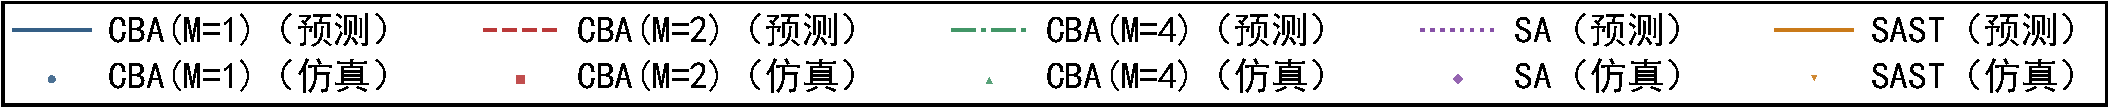
\includegraphics[width=0.99\textwidth, trim=0 0 0 0, clip]{figure/chap5/shared_legend.pdf} \\
    
    % 第二行：子图并排
    \subfloat{
        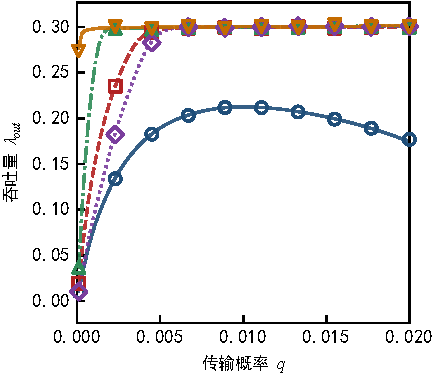
\includegraphics[width=0.49\textwidth]{figure/chap5/5_3_metric_throughput.pdf}
        \label{fig:ai_vs_sim_uniform_003_thr}
    }
    \subfloat{
        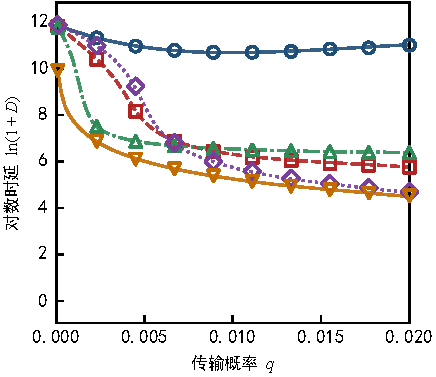
\includegraphics[width=0.49\textwidth]{figure/chap5/5_3_metric_delay.pdf}
        \label{fig:ai_vs_sim_uniform_003_delay}
    } \\
    
    % 第三行：子图并排
    % \subfloat[公平性 $J$]{
    %     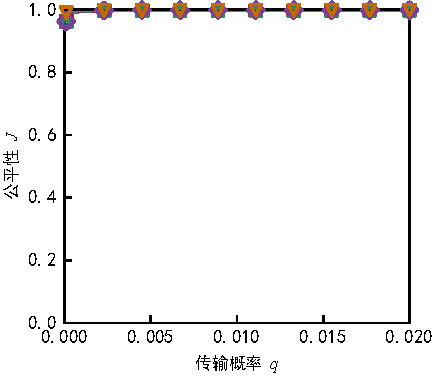
\includegraphics[width=0.49\textwidth]{figure/chap5/5_3_metric_fairness.pdf}
    %     \label{fig:ai_vs_sim_uniform_003_fairness}
    % }
    \subfloat{
        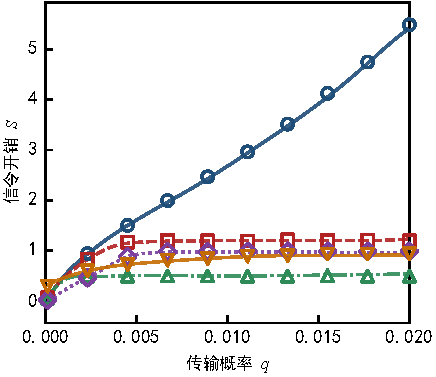
\includegraphics[width=0.49\textwidth]{figure/chap5/5_3_metric_signaling.pdf}
        \label{fig:ai_vs_sim_uniform_003_signaling}
    }
    
    \caption{均匀流量、$\lambda=0.003$ 场景下的模型预测（理论值）与仿真结果（离散点）对比。}
    \label{fig:ai_vs_sim_uniform_003}
\end{figure}

\begin{figure}[t]
    \centering
    % 第一行：全局共享图例（缩放因子根据实际大小微调，这里设为 0.95 避免溢出）
    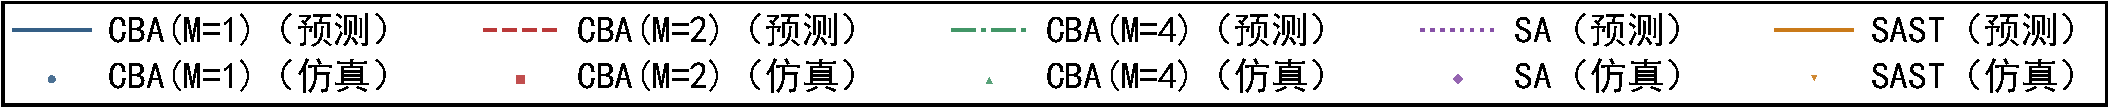
\includegraphics[width=0.99\textwidth, trim=0 0 0 0, clip]{figure/chap5/shared_legend.pdf} \\
	
	\subfloat[吞吐优先]{
		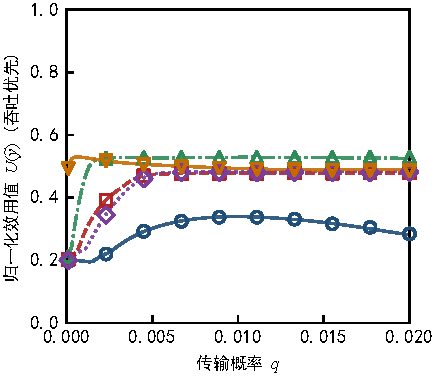
\includegraphics[width=0.48\textwidth]{figure/chap5/5_3_utility_throughput_prio.pdf}
		\label{fig:utility_priority_uniform_003_thr}
	}
	\hfill
	\subfloat[时延优先]{
		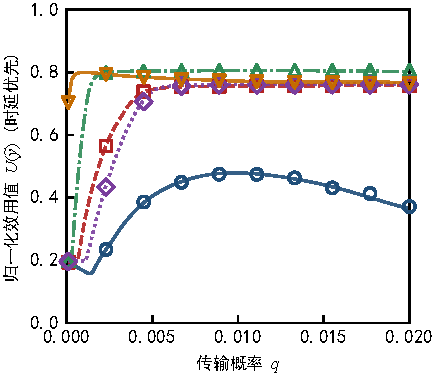
\includegraphics[width=0.48\textwidth]{figure/chap5/5_3_utility_delay_prio.pdf}
		\label{fig:utility_priority_uniform_003_delay}
	}
	\hfill
	\subfloat[信令优先]{
		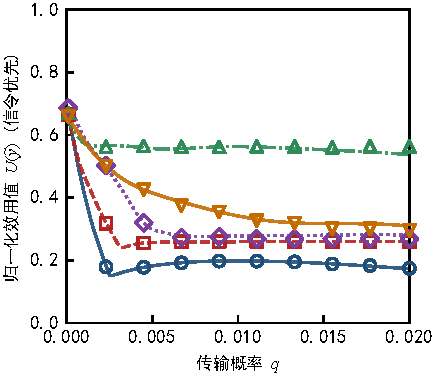
\includegraphics[width=0.55\textwidth]{figure/chap5/5_3_utility_signaling_prio.pdf}
		\label{fig:utility_priority_uniform_003_signaling}
	}
	\caption{均匀流量、$\lambda=0.003$ 场景下，不同权重偏好的综合效用 $U$ 对比。}
	\label{fig:utility_priority_uniform_003}
\end{figure}
\subsection{性能预测模型曲线一致性与效用曲线对比说明}
本小节以均匀流量、单节点到达率 $\lambda=0.003$ 为例，对不同协议参数 $q$ 下的性能曲线进行可视化对比。图~\ref{fig:ai_vs_sim_uniform_003} 中实线为预测、离散点为仿真结果，吞吐量、时延与信令开销三类指标在参数区间内的变化趋势一致，峰值与拐点位置可对齐。公平性指标 $J_T$ 在各配置下基本接近 1、区分度较低，故不再单独绘制其曲线图。

进一步，为反映不同业务偏好下的综合性能，本节同时考察效用函数 $U(\tilde{\mathbf{y}})$ 的变化趋势，并将三种典型权重配置合并展示：吞吐优先、时延优先与信令优先。对应曲线见图~\ref{fig:utility_priority_uniform_003} 的三个子图。三条曲线在峰值位置与拐点处的差异，体现了权重设置对最优参数选择的影响：吞吐优先更倾向于高负载区间的参数组合；时延优先与信令优先则更偏向保守配置以降低排队与控制开销。该对比说明在统一性能预测模型输出基础上，仅需调整权重即可实现面向不同业务目标的快速策略切换。



\section{基于性能预测模型的快速搜索与预测}
在性能预测模型 $f_{\phi}$ 训练完成后，协议优化问题可转化为单次决策窗口内的参数搜索问题。给定业务场景的流量特征 $\mathbf{x}_{\text{traffic}}$，目标是求得统一参数向量 $\mathbf{x}_{\text{proto}}^*$, 即：
\begin{equation}
	\mathbf{x}_{\text{proto}}^* = \arg\max_{\mathbf{x}_{\text{proto}}} U\big(f_{\phi}(\mathbf{x}_{\text{traffic}}, \mathbf{x}_{\text{proto}}, \dots)\big)
\end{equation}
由于 $f_{\phi}$ 的评估开销较低，本文采用直接网格搜索以保证可复现性。针对混合离散—连续参数空间，该方法在候选协议与参数域内逐点评估并选择效用最大值。

在实际业务场景中，网络流量类型与强度具备显著的动态时变性，且协议切换决策与流量突变往往非同步。为贴合工程流程，本文采用滑动观测窗口在线更新流量特征，并在每个决策时刻执行一次快速搜索。具体流程为：
\begin{enumerate}[leftmargin=*]
	\item \textbf{状态观测}：在窗口 $[t-\Delta t, t]$ 内统计流量特征 $\mathbf{x}_{\text{traffic}}$；
	\item \textbf{直接搜索}：对 $\mathcal{P}$ 中各协议进行枚举，并在其参数域内快速搜索；
	\item \textbf{协议自切换}：选择效用最高且满足约束的协议与参数，触发协议切换并下发配置；
\end{enumerate}

为保证对比结果的可复现性与逻辑一致性，本文构建两类验证场景。每类场景均包含连续 10 个观测窗口，单窗口长度为 $3\times10^5$ 个时隙；协议切换与窗口边界同步，决策周期同样设为 $3\times10^5$ 个时隙。每个窗口内均采用直接搜索获得性能预测模型推荐策略，并以离线穷举得到的近似最优效用作为参考上界。

\textbf{场景一：均匀流量、强度递变。} 该场景中流量类型固定为均匀到达（U），仅按预设序列调整归一化平均到达率 $\hat{\lambda}$。具体窗口配置见表~\ref{tab:chap5_scene1_windows}。该序列覆盖低、中、高多档负载，并包含升载与降载过程，用于评估流量形态固定条件下各协议对强度动态的适配能力。

\begin{table}[htbp]
\centering
\caption{场景一的窗口配置（均匀流量、强度递变）}
\label{tab:chap5_scene1_windows}
\renewcommand{\arraystretch}{1.15}
\small
\setlength{\tabcolsep}{5pt}
\begin{tabular}{c c c c}
\toprule
\textbf{窗口} & \textbf{时间区间 $t$} & \textbf{流量类型} & \textbf{$\hat{\lambda}$} \\
\midrule
1  & $[0,3\times10^5)$    & U & 0.10 \\
2  & $[3\times10^5,6\times10^5)$  & U & 0.20 \\
3  & $[6\times10^5,9\times10^5)$  & U & 0.30 \\
4  & $[9\times10^5,12\times10^5)$ & U & 0.70 \\
5  & $[12\times10^5,15\times10^5)$ & U & 0.45 \\
6  & $[15\times10^5,18\times10^5)$ & U & 0.50 \\
7  & $[18\times10^5,21\times10^5)$ & U & 0.55 \\
8  & $[21\times10^5,24\times10^5)$ & U & 0.80 \\
9  & $[24\times10^5,27\times10^5)$ & U & 0.25 \\
10 & $[27\times10^5,30\times10^5)$ & U & 0.10 \\
\bottomrule
\end{tabular}
\end{table}

\textbf{场景二：流量类型与强度联合变化。} 该场景中流量形态与归一化平均到达率在 10 个窗口内同步变化，覆盖均匀（U）、突发（B）、周期（P）三类到达过程，构成“低负载→中负载→高负载→恢复”的循环序列。具体窗口配置见表~\ref{tab:chap5_scene2_windows}。该序列通过引入形态切换及强度升降过程，用于检验系统在流量类型与强度同时变化条件下的综合适配能力。

\begin{table}[htbp]
\centering
\caption{场景二的窗口配置（流量类型与强度联合变化）}
\label{tab:chap5_scene2_windows}
\renewcommand{\arraystretch}{1.15}
\small
\setlength{\tabcolsep}{5pt}
\begin{tabular}{c c c c}
\toprule
\textbf{窗口} & \textbf{时间区间 $t$} & \textbf{流量类型} & \textbf{$\hat{\lambda}$} \\
\midrule
1  & $[0,3\times10^5)$    & U & 0.10 \\
2  & $[3\times10^5,6\times10^5)$  & B & 0.30 \\
3  & $[6\times10^5,9\times10^5)$  & P & 0.50 \\
4  & $[9\times10^5,12\times10^5)$ & U & 0.70 \\
5  & $[12\times10^5,15\times10^5)$ & B & 0.50 \\
6  & $[15\times10^5,18\times10^5)$ & P & 0.30 \\
7  & $[18\times10^5,21\times10^5)$ & U & 0.20 \\
8  & $[21\times10^5,24\times10^5)$ & B & 0.60 \\
9  & $[24\times10^5,27\times10^5)$ & P & 0.40 \\
10 & $[27\times10^5,30\times10^5)$ & U & 0.15 \\
\bottomrule
\end{tabular}
\end{table}

为明确改进来源，本文设置两类基线策略：
\begin{itemize}[leftmargin=*]
	\item \textbf{基线1：单一协议固定参数。} 采用 SA 协议，传输概率 $q=0.01$ 恒定不变，用作静态配置参考。
	\item \textbf{基线2：协议固定、参数可调。} 固定协议为 CBA，仅在协议内调参。对 $q$ 进行网格穷举（有效区间内均匀取 100 个采样点，并在峰值邻域额外加密 50 点），$M\in\{1,2,4\}$ 逐一遍历，取效用最大者作为该窗口的最优配置。
\end{itemize}

实验流程包括生成流量变化序列、提取窗口特征、在线搜索与协议切换，以及对比最优效用曲线与指标趋势。对上述两种场景分别进行实验，结果分别如图~\ref{fig:utility_vs_traffic_uniform} 与图~\ref{fig:utility_vs_traffic_mixed} 所示。

\begin{figure}[t]
	\centering
	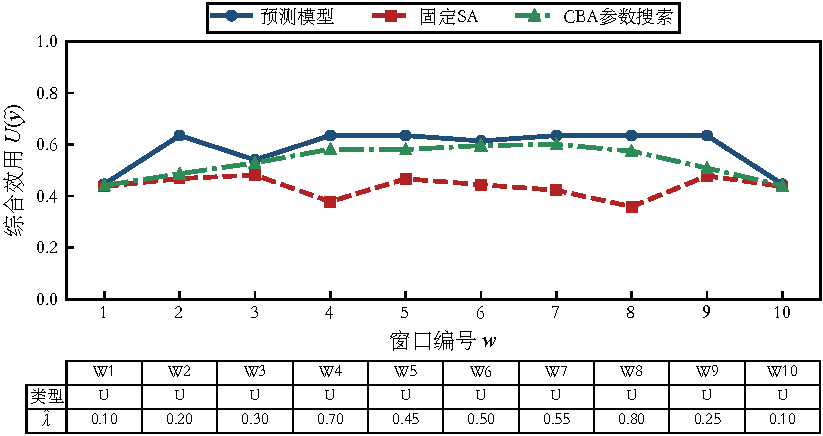
\includegraphics[width=0.99\textwidth]{figure/chap5/utility_dynamic_uniform_0315.pdf}
	\caption{场景一下性能预测模型推荐策略与基线策略的效用对比。横坐标表示按时序排列的协议切换窗口编号，纵坐标表示对应的综合效用 $U(\tilde{\mathbf{y}})$。}
	\label{fig:utility_vs_traffic_uniform}
\end{figure}

\begin{figure}[t]
	\centering
	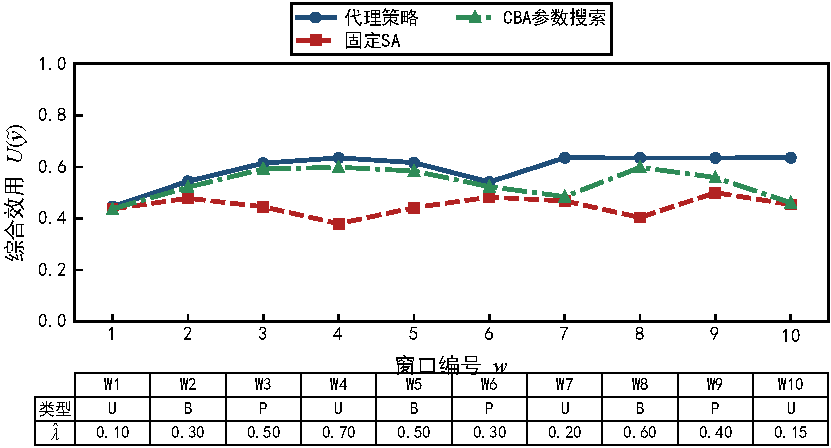
\includegraphics[width=0.99\textwidth]{figure/chap5/utility_dynamic_combined_0315.pdf}
	\caption{场景二下性能预测模型推荐策略与基线策略的效用对比。横坐标表示按时序排列的协议切换窗口编号，纵坐标表示对应的综合效用 $U(\tilde{\mathbf{y}})$。}
	\label{fig:utility_vs_traffic_mixed}
\end{figure}




\section{本章小结}

本章提出了一种基于监督学习的智能协议与参数联合选择方法，旨在解决传统单一接入协议在复杂多变业务场景下的性能局限性。首先，我们设计了一个统一的接入框架，通过标准化的输入特征向量，对不同的业务流量、网络规模和协议参数进行统一建模。随后，为克服传统网络仿真的高时间成本，我们构建了性能预测模型，并利用多任务深度神经网络学习并复现从输入特征到多维性能指标的复杂映射关系。最后，基于训练好的、能够进行毫秒级预测的性能预测模型，将原先难以处理的协议优化问题转化为一个可由高效搜索算法求解的数学问题。

综上所述，本章通过统一框架设计、性能预测模型构建与快速优化求解，为实现随机接入机制的智能化和自适应化提供了完整的理论与实践基础。
